% !TeX spellcheck = en_GB
\section{Large scale circulation} \label{sec:largeScale}
\textcolor{red}{Some text to get a flow.}
\begin{figure}
	\centering
	%%% dyntropo %%%%
	\begin{subfigure}[b]{0.49\textwidth}
		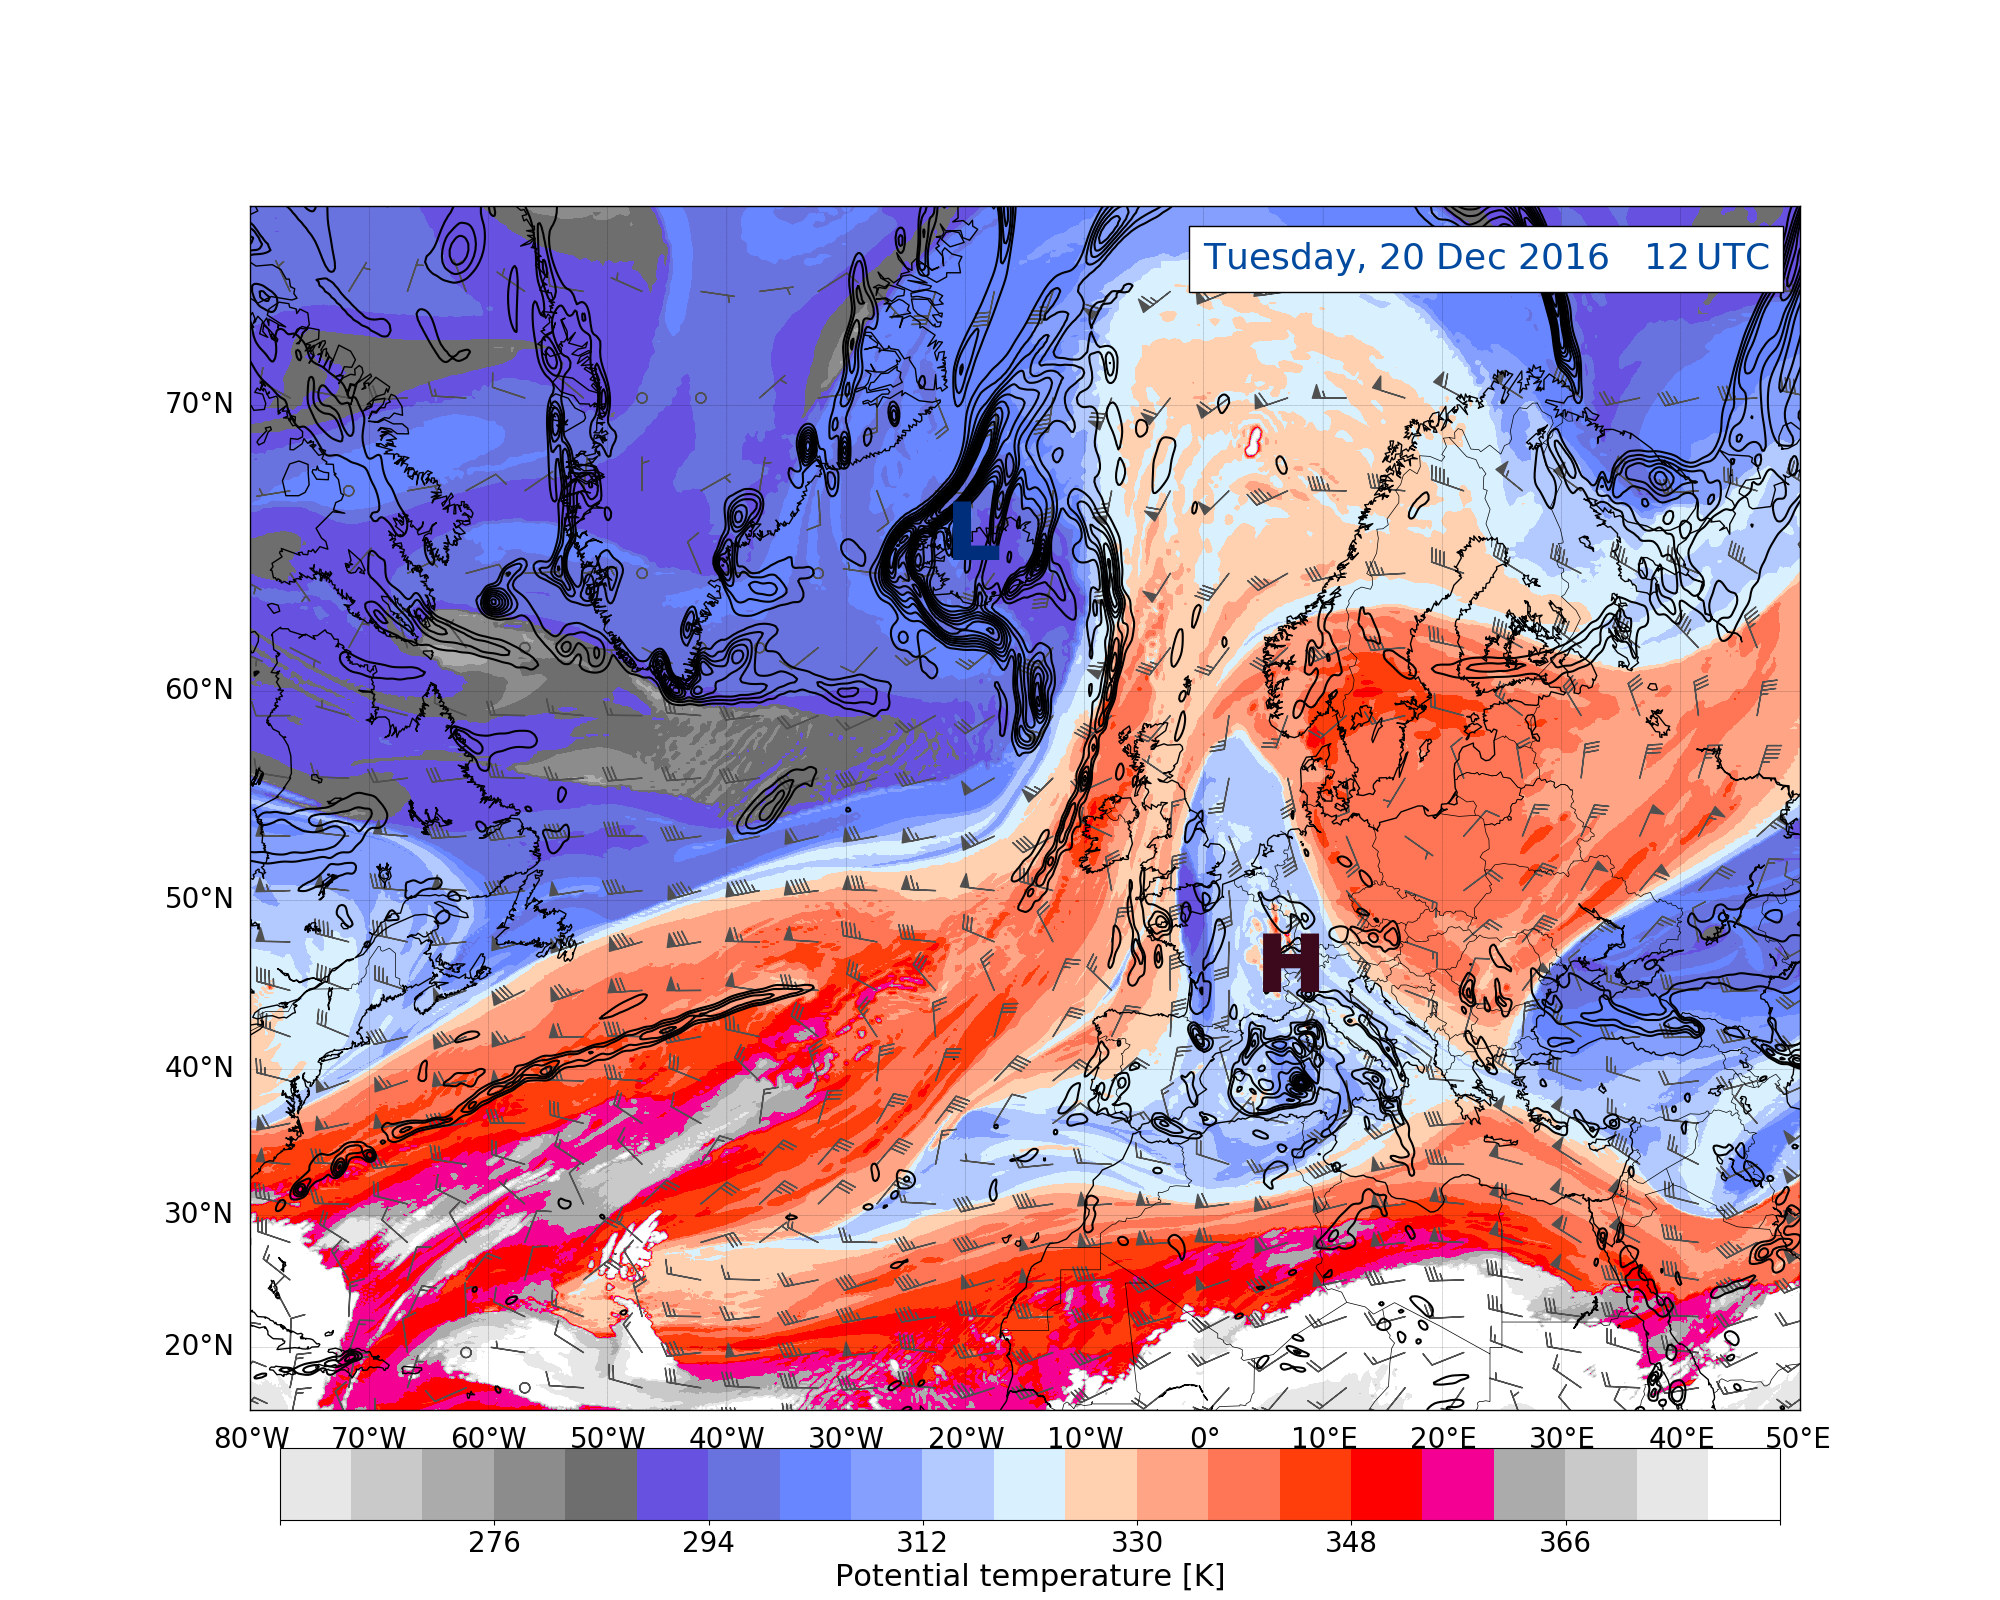
\includegraphics[trim={4.2cm 0cm 4.3cm 5.1cm},clip,
		width=\textwidth]{./fig_DynTropo/20161220_12}
		\caption{} \label{fig:DT20}
	\end{subfigure}
	\begin{subfigure}[b]{0.49\textwidth}
		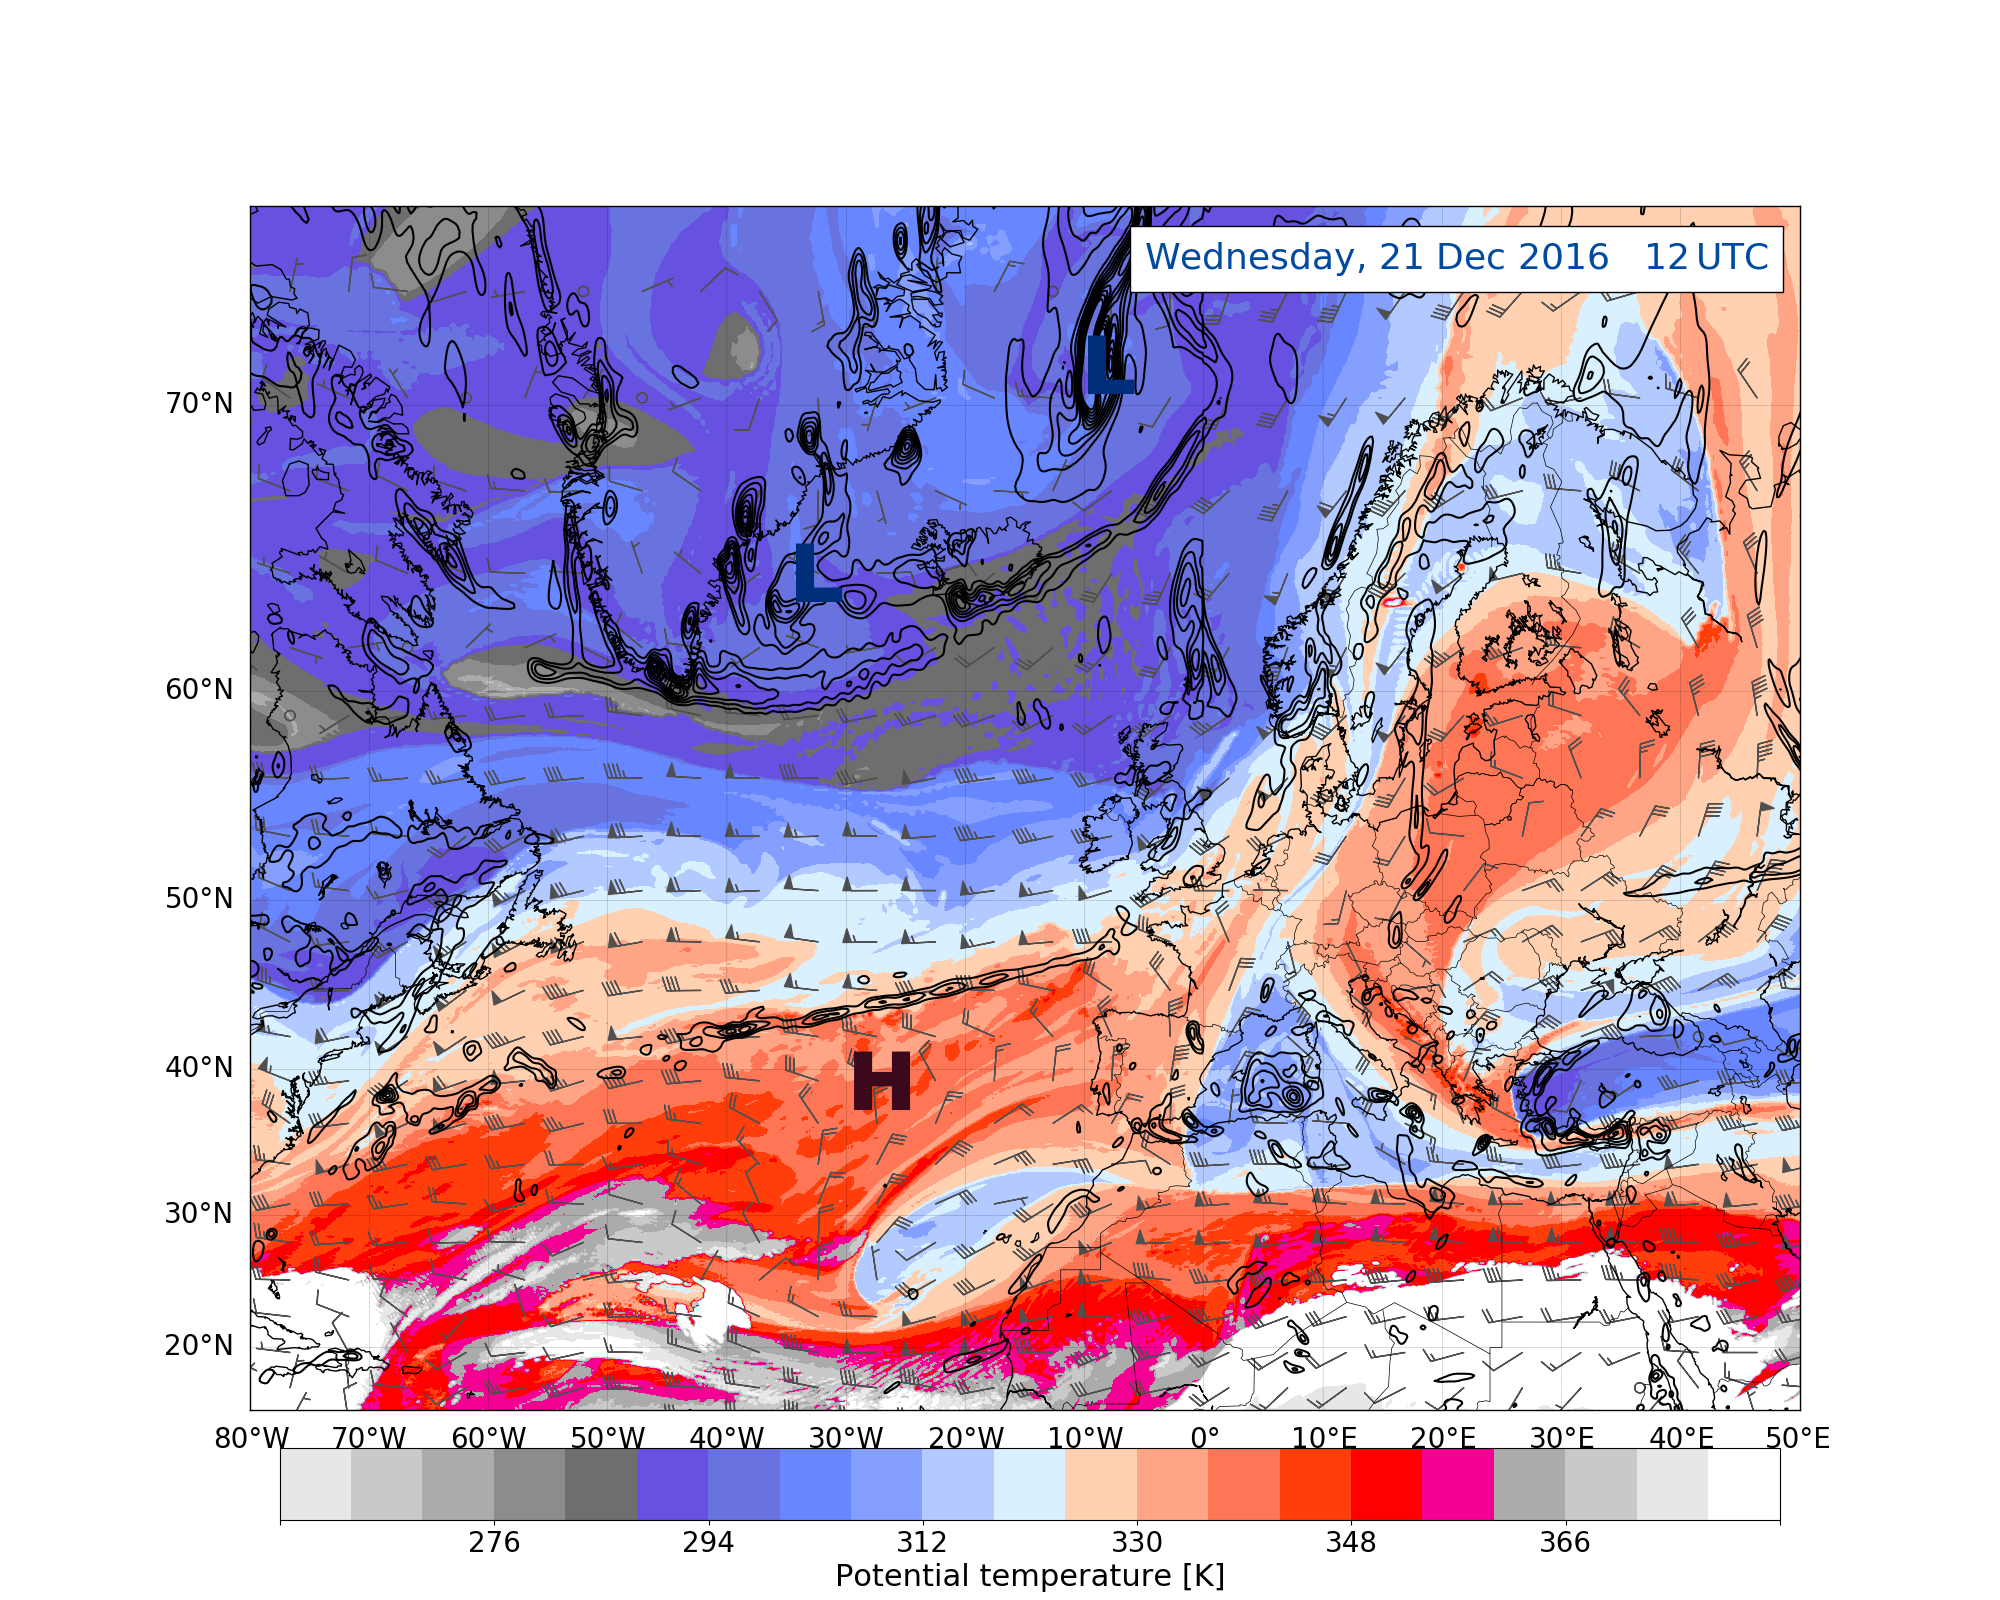
\includegraphics[trim={4.2cm 0cm 4.3cm 5.1cm},clip,
		width=\textwidth]{./fig_DynTropo/20161221_12}
		\caption{} \label{fig:DT21}
	\end{subfigure}
	%%% geopot %%%%
	\begin{subfigure}[b]{0.49\textwidth}
		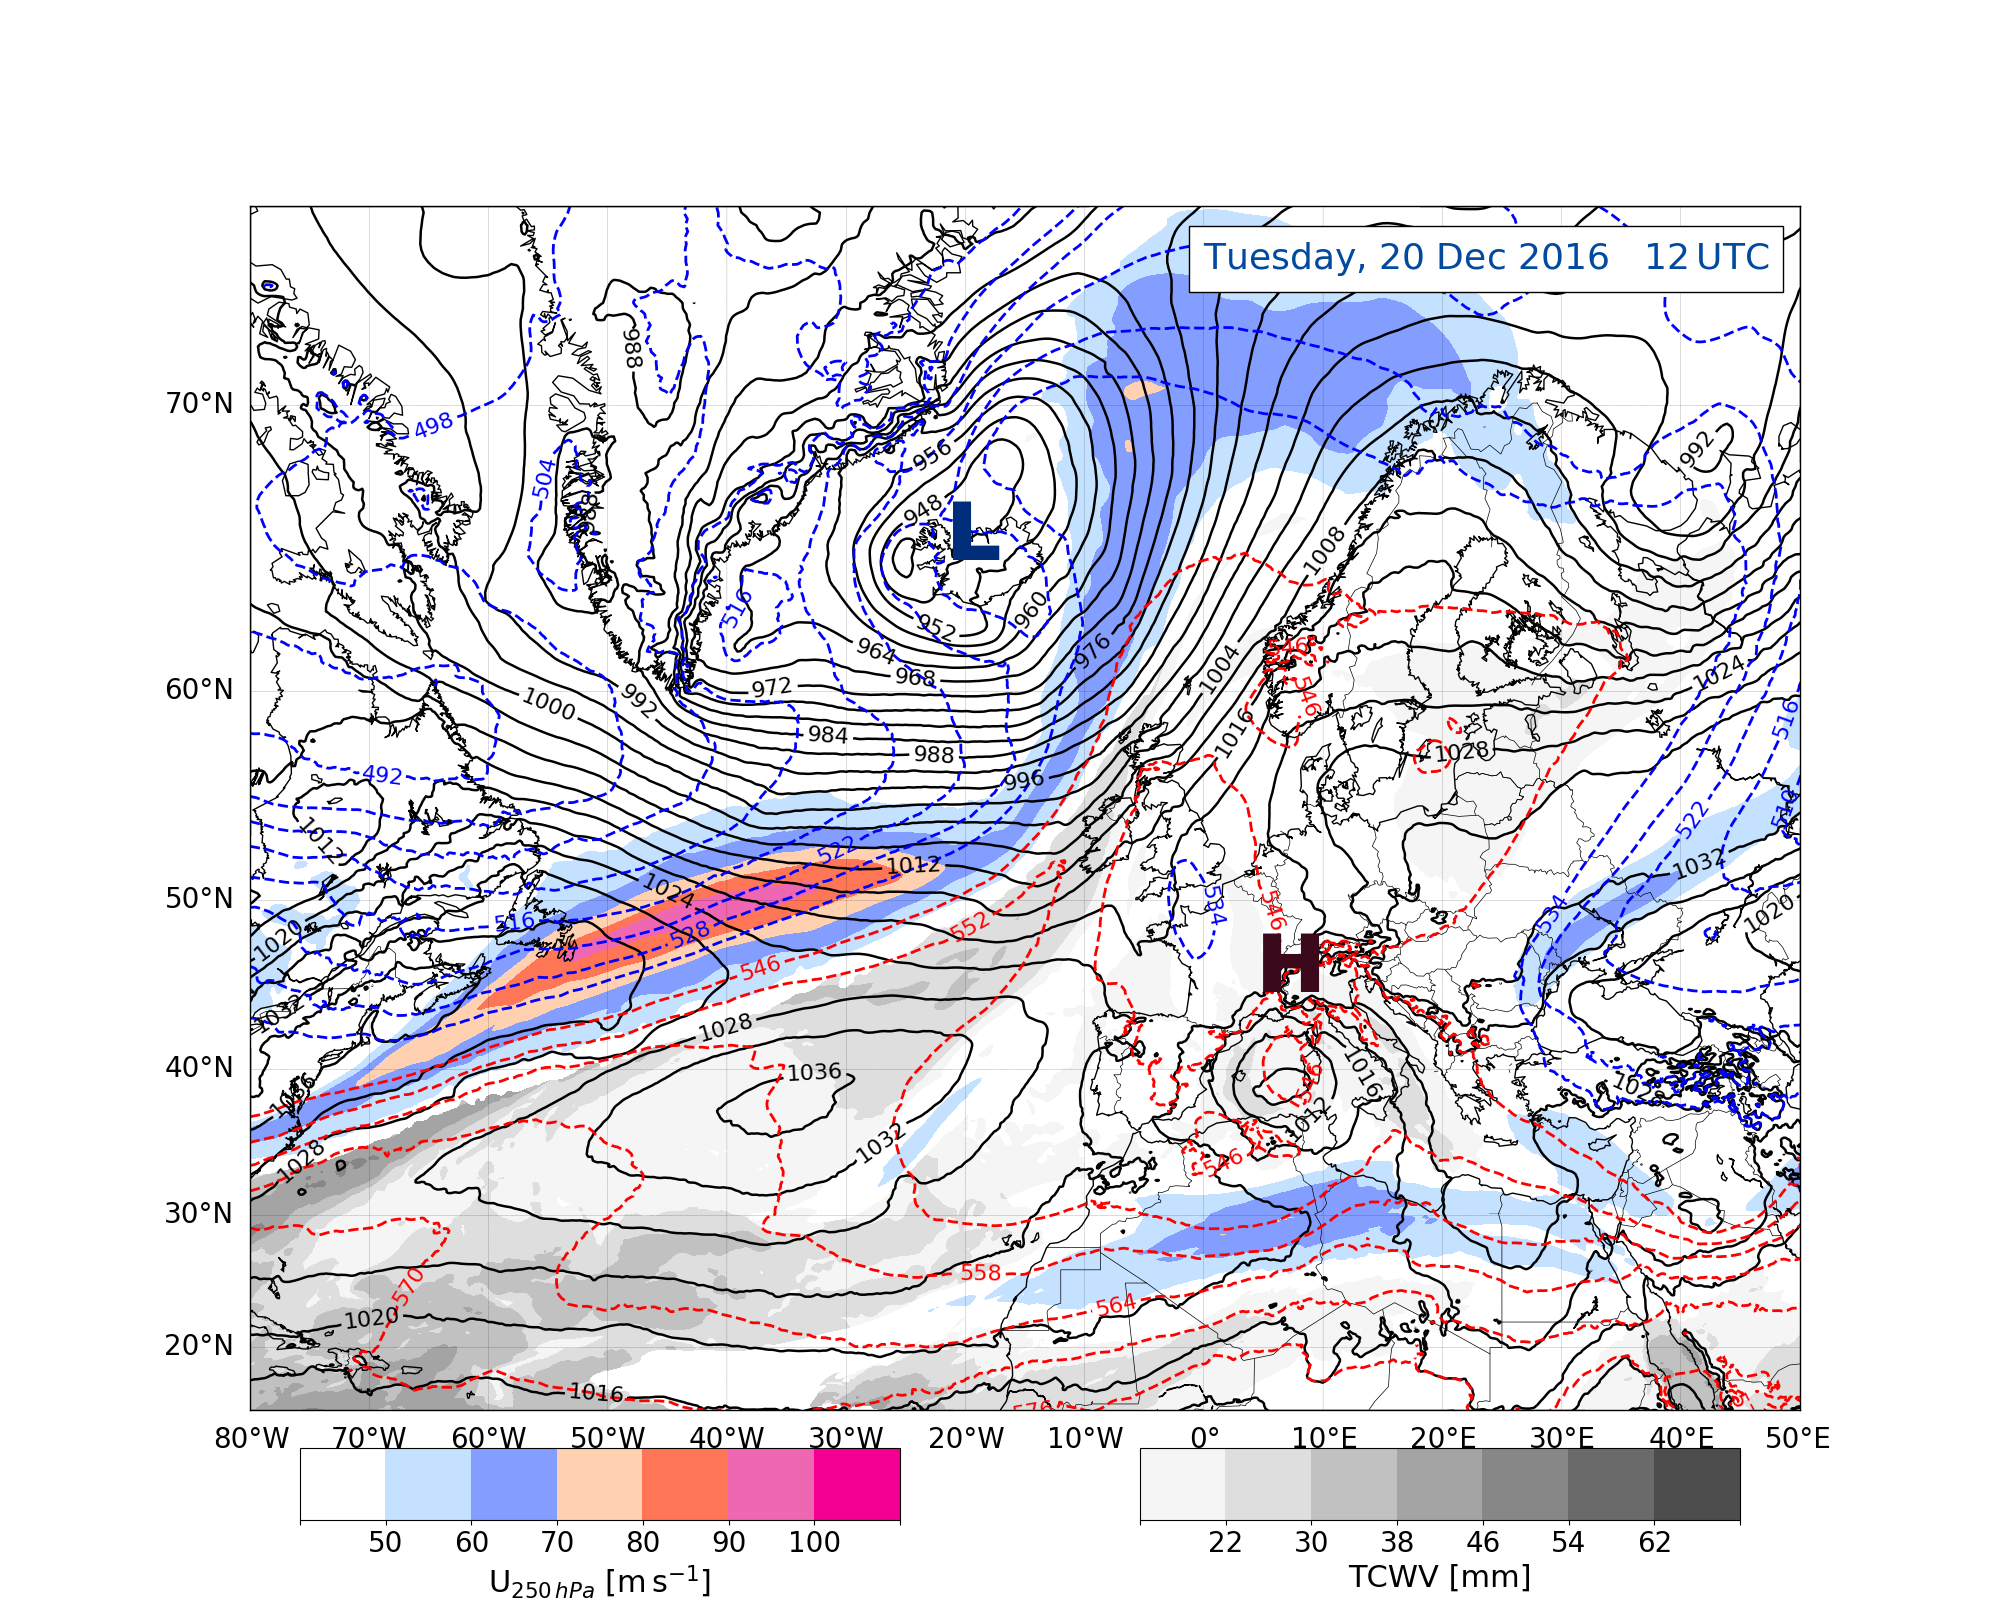
\includegraphics[trim={4.2cm 0cm 4.3cm 5.1cm},clip,
		width=\textwidth]{./fig_Geopot_Jet/20161220_12}
		\caption{} \label{fig:GP20}
	\end{subfigure}
	\begin{subfigure}[b]{0.49\textwidth}
		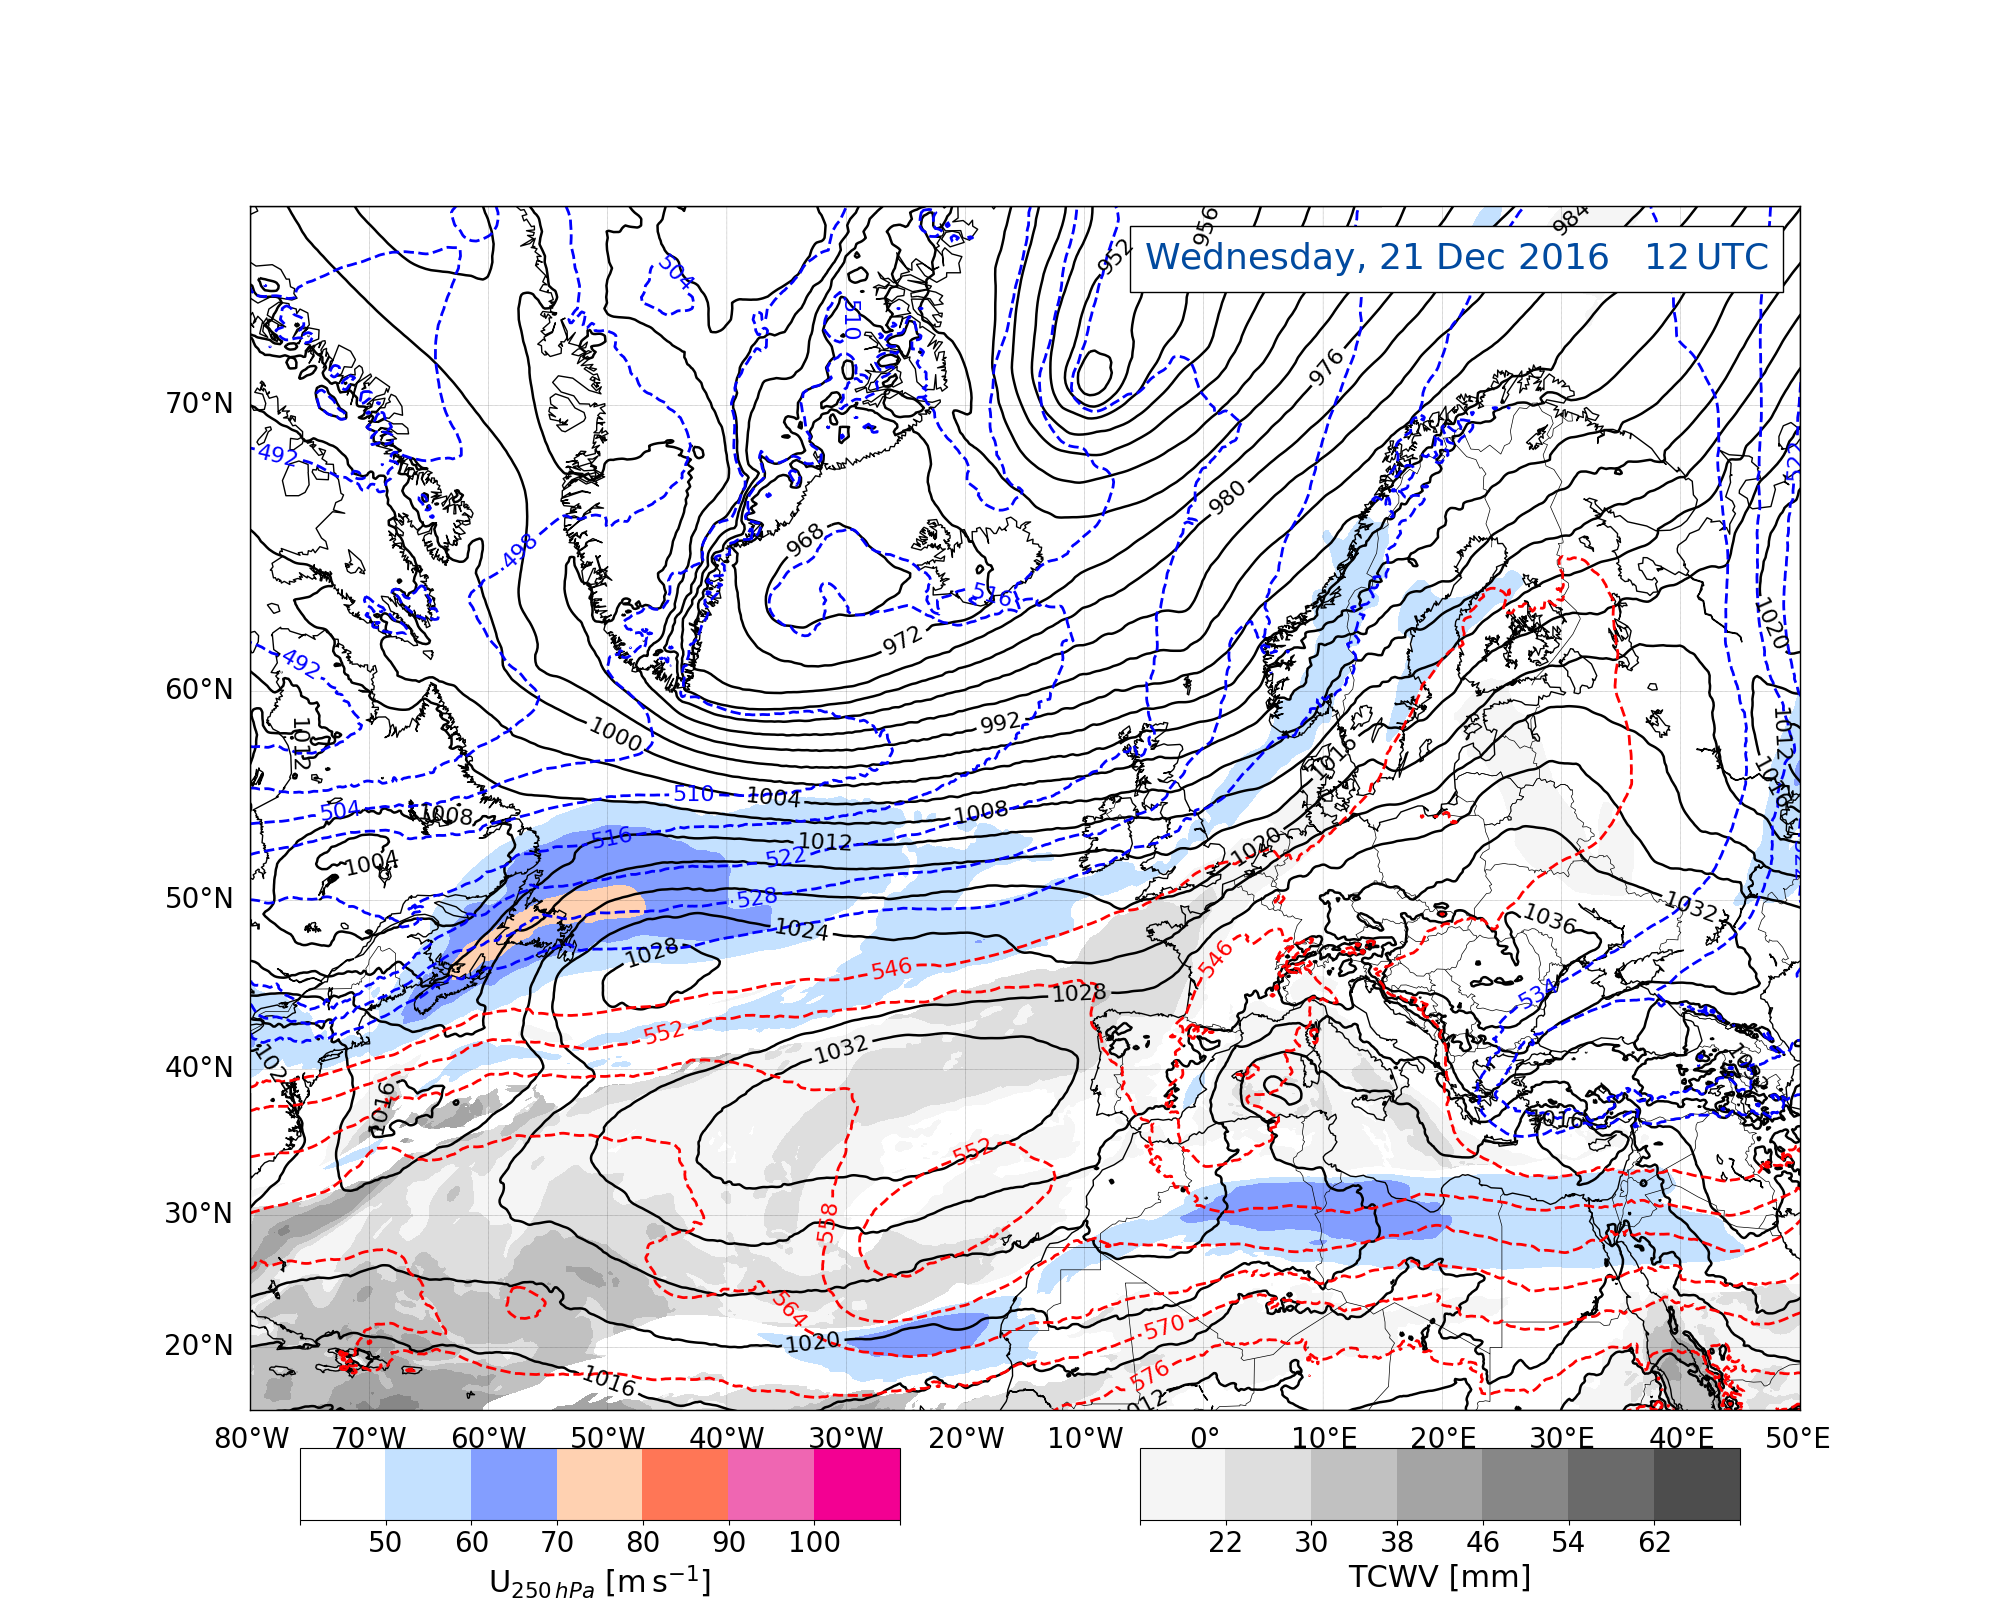
\includegraphics[trim={4.2cm 0cm 4.3cm 5.1cm},clip,
		width=\textwidth]{./fig_Geopot_Jet/20161221_12}
		\caption{} \label{fig:GP21}
	\end{subfigure}
	%%% local obs %%%%
	\begin{subfigure}[b]{0.49\textwidth}
		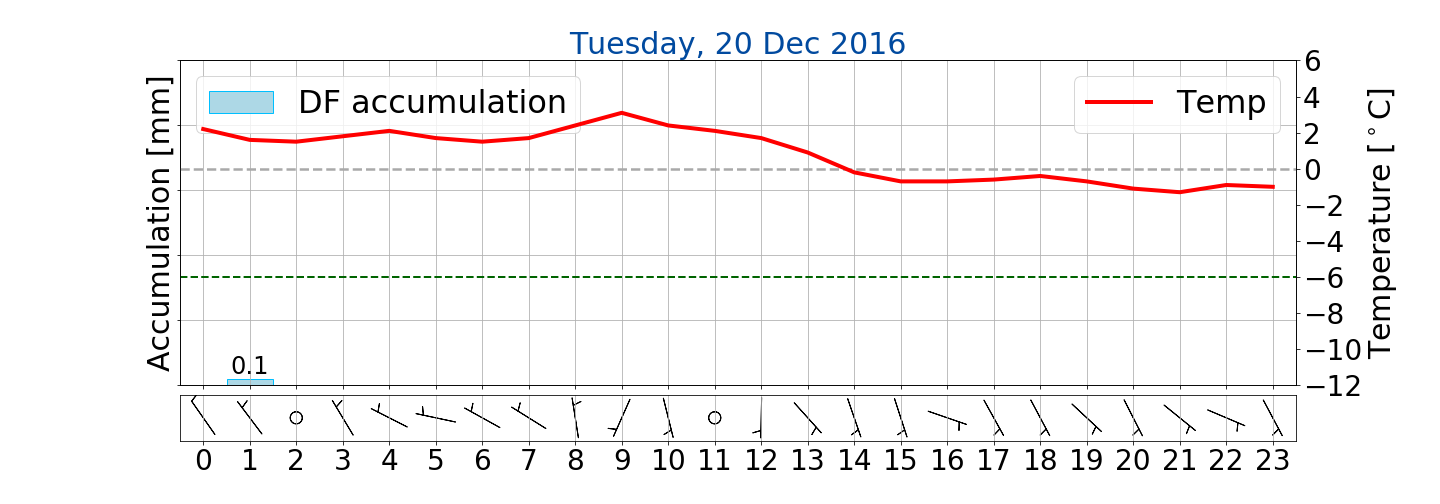
\includegraphics[trim={4.9cm 1.cm 1.5cm 1cm},clip,
		width=\textwidth]{./fig_weathermast/T_P_U_20161220}
		\caption{} \label{fig:TPU20}
	\end{subfigure}
	\begin{subfigure}[b]{0.49\textwidth}
		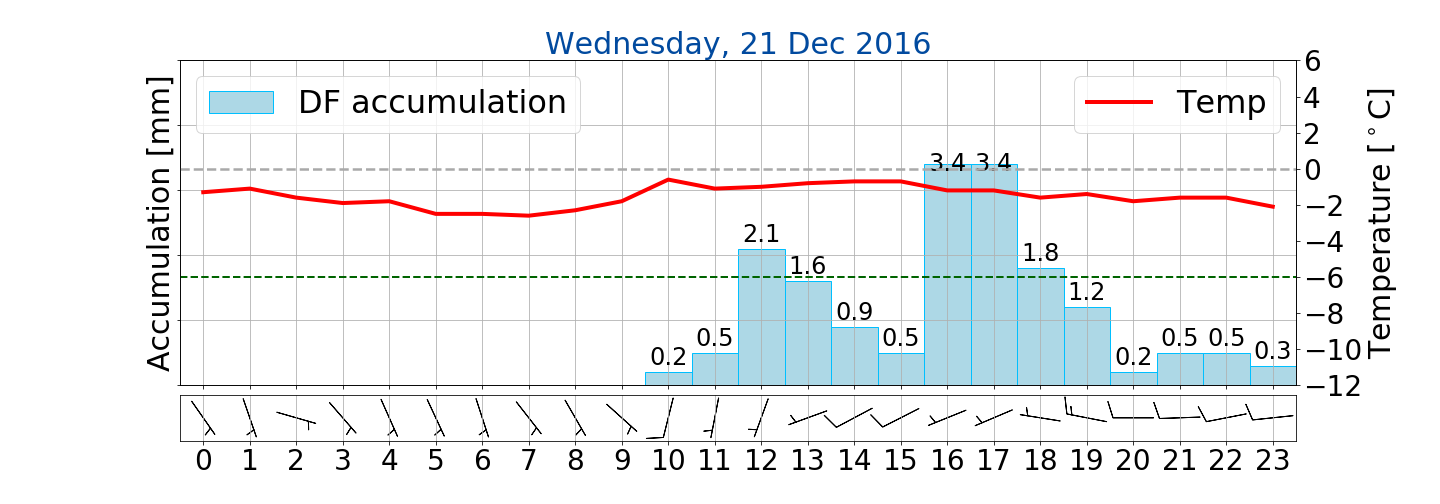
\includegraphics[trim={4.9cm 1.cm 1.5cm 1cm},clip,
		width=\textwidth]{./fig_weathermast/T_P_U_20161221}
		\caption{} \label{fig:TPU21}
	\end{subfigure}
\end{figure}
%%% 21/12
% 21/00
% Westerly flow, perfect for orographic lifting
% → lots of moisture (check for correct values)
% Cold air goes right over Norway 
% → probably snow
% 21/18
% Low forming right at the main baroclinic zone (~45°N, south of Greenland)
% Formation @ the right entrance region of the jet, which helps for lifting
\subsection*{\SI{21}{\dec}}
The dynamic tropopause map in \Cref{fig:DT21} shows that Norway is influenced by a change of elevated tropopause to a suppressed tropopause during \SIrange{20}{21}{\dec}. Hence the potential vorticity changed from positive to negative at the tropopause and cold air stretches right over Norway.
A good amount of moisture is transported from the low latitudes to high latitudes, influencing Norway’s' west coast. This can be seen in the surface maps (\Cref{fig:GP21}) as well as in the atmospheric river maps (\Cref{fig:AR21}). The westerly flow in \Cref{fig:GP21} is conducive to orographic lifting. The precipitation was probably snow when having a look at the moisture content and the cold air. The change from warm air to cold air can also be observed in the time series of temperature in \Cref{fig:TPU21}. And the westerly flow, combined with a good amount of vapour transport from the tropics led to orographic lifting and precipitation at the Haukeliseter site. 
At around \ang{60}{\,W} a formation of a cyclone at the baroclinic zone can be implied.  

\begin{figure}
	\centering
	%%% dyntropo %%%%
	\begin{subfigure}[b]{0.49\textwidth}
		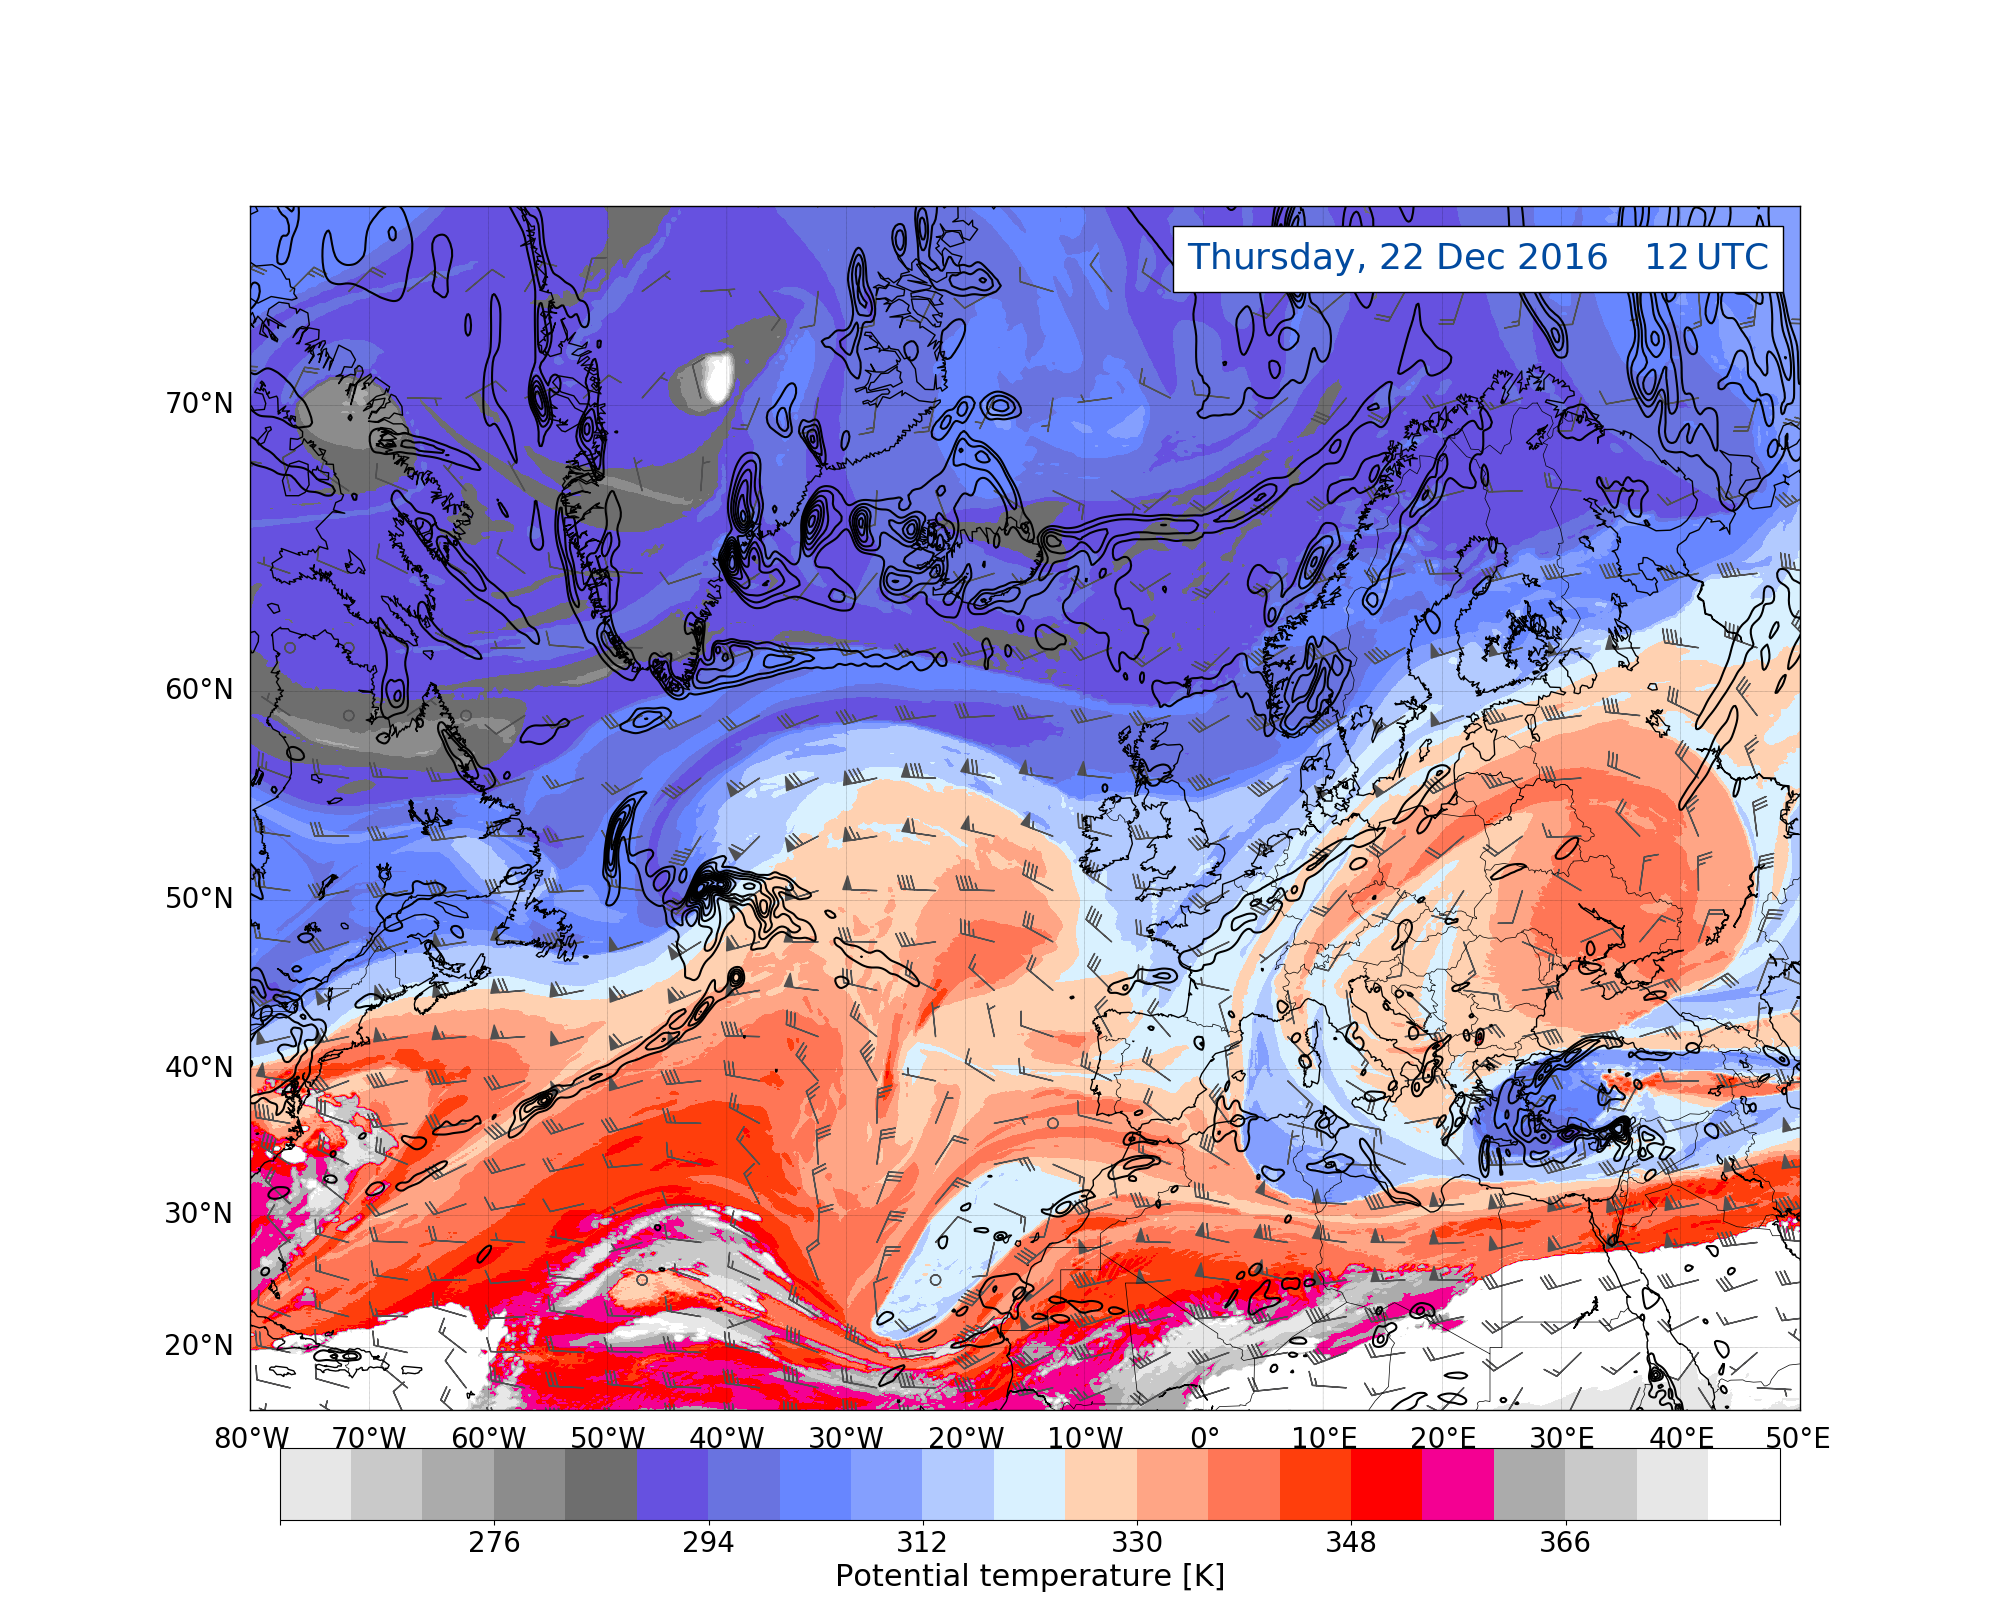
\includegraphics[trim={4.2cm 0cm 4.3cm 5.1cm},clip,
		width=\textwidth]{./fig_DynTropo/20161222_12}
		\caption{} \label{fig:DT22}
	\end{subfigure}
	%     \begin{subfigure}[b]{0.49\textwidth}
	%     	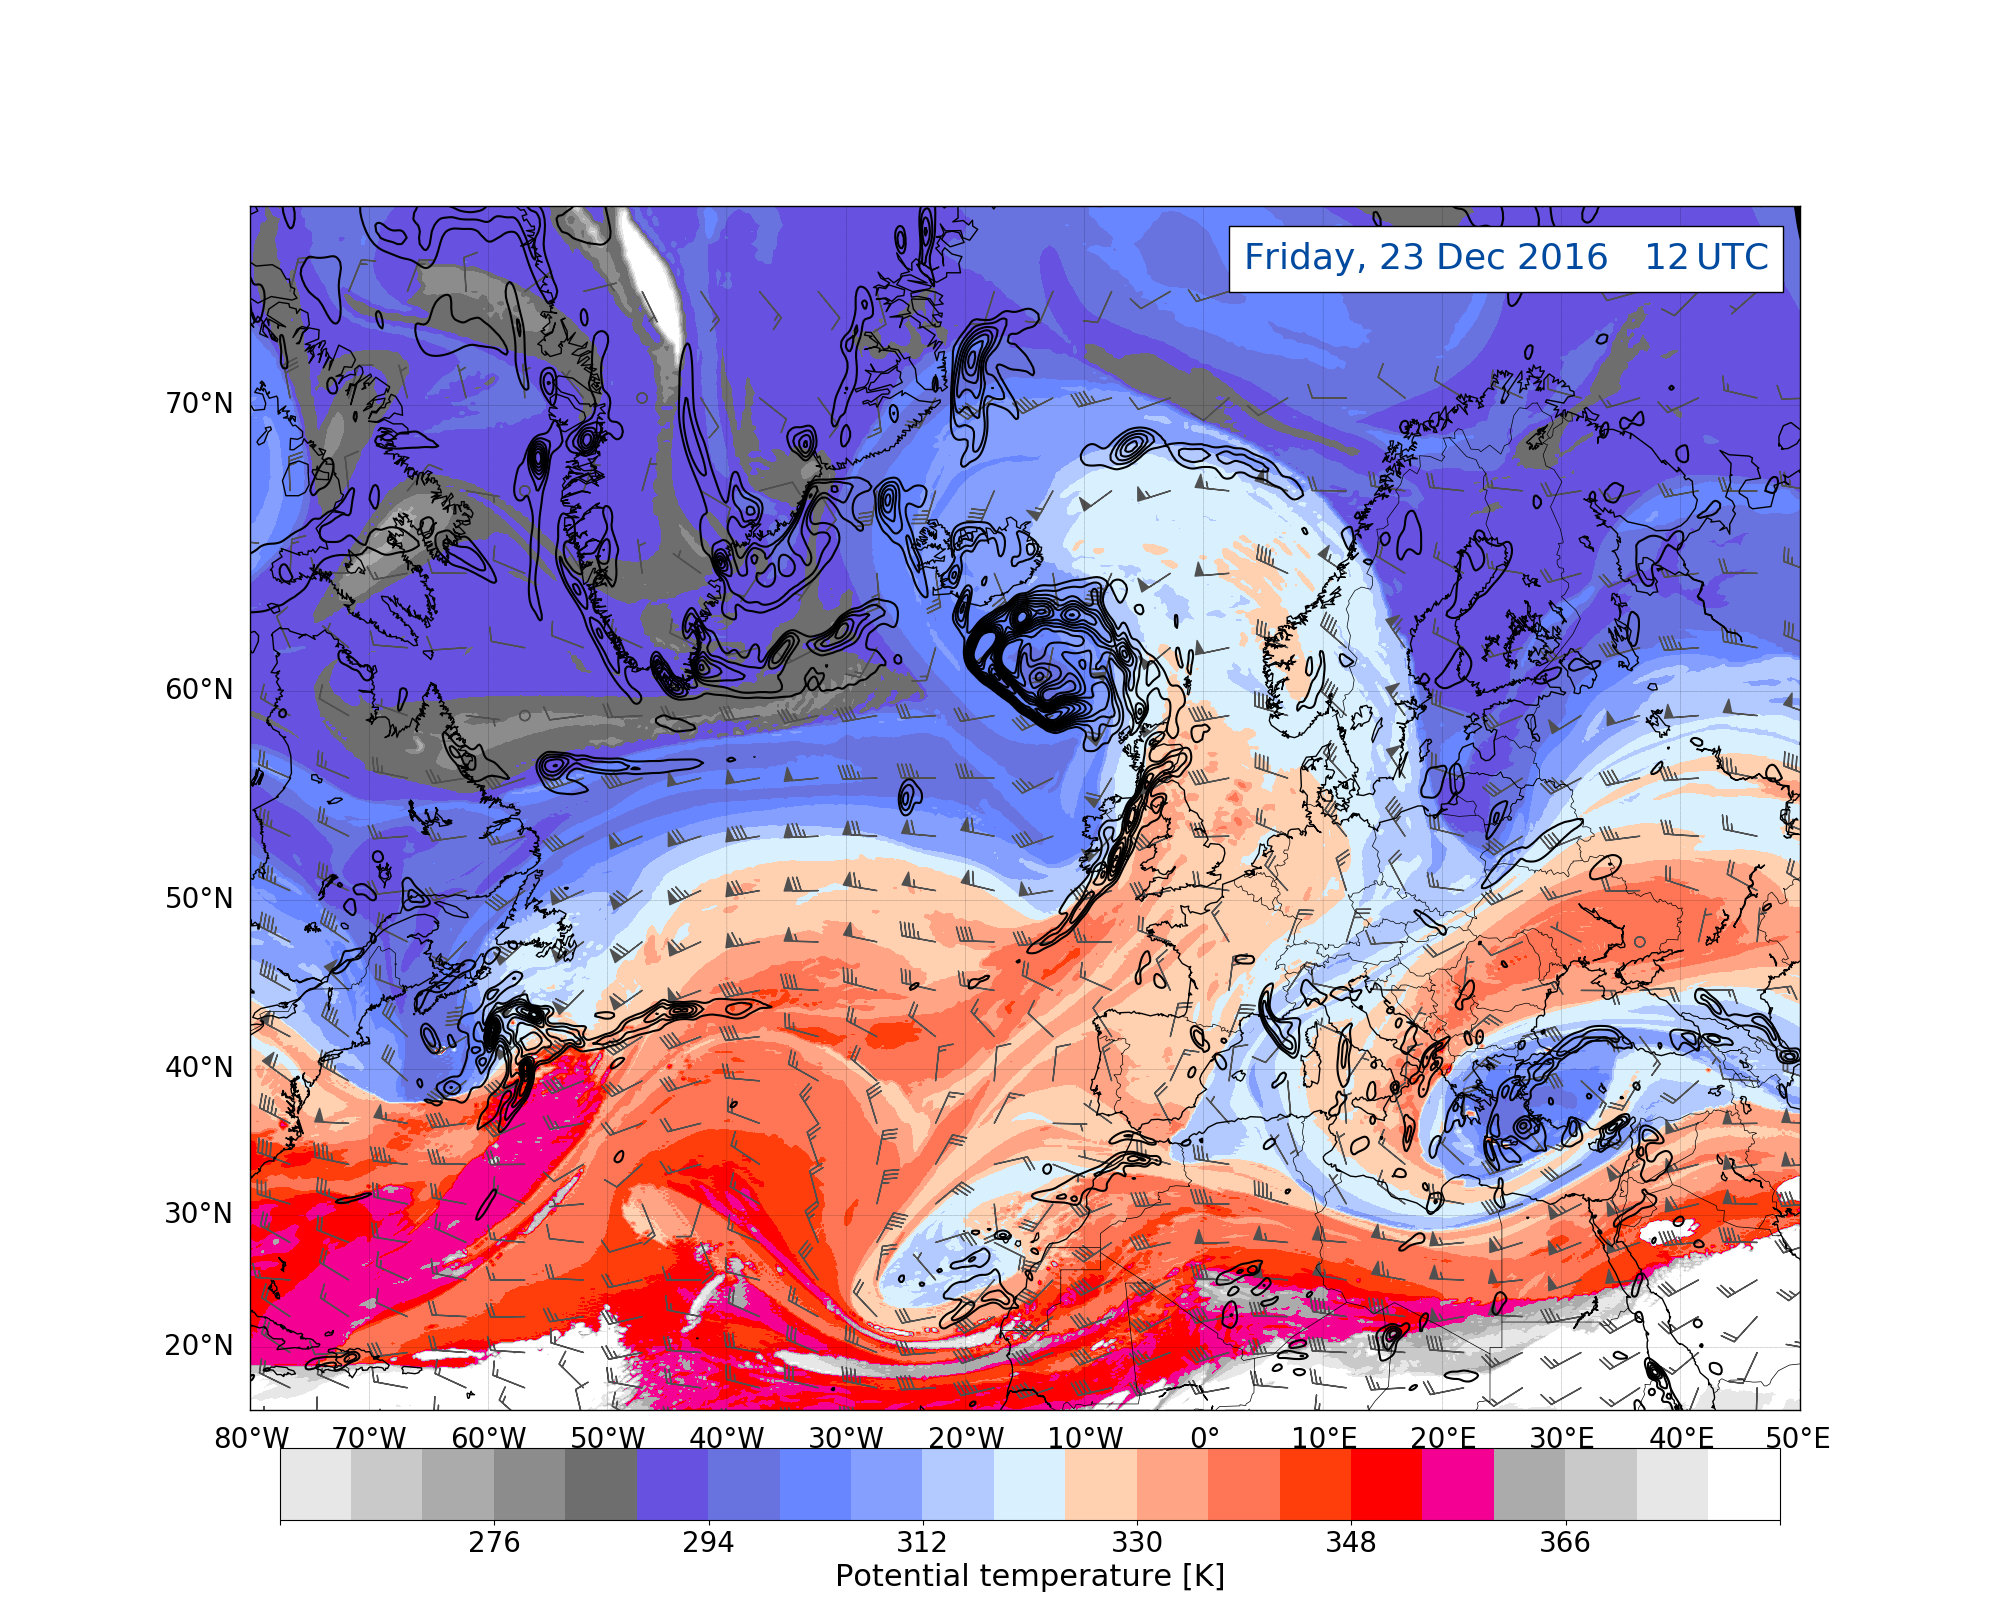
\includegraphics[trim={4.2cm 0cm 4.3cm 5.1cm},clip,
	% 		width=\textwidth]{./fig_DynTropo/20161223_12}
	% 		\caption{} \label{fig:DT23}
	%     \end{subfigure}
	%%% geopot %%%%
	\begin{subfigure}[b]{0.49\textwidth}
		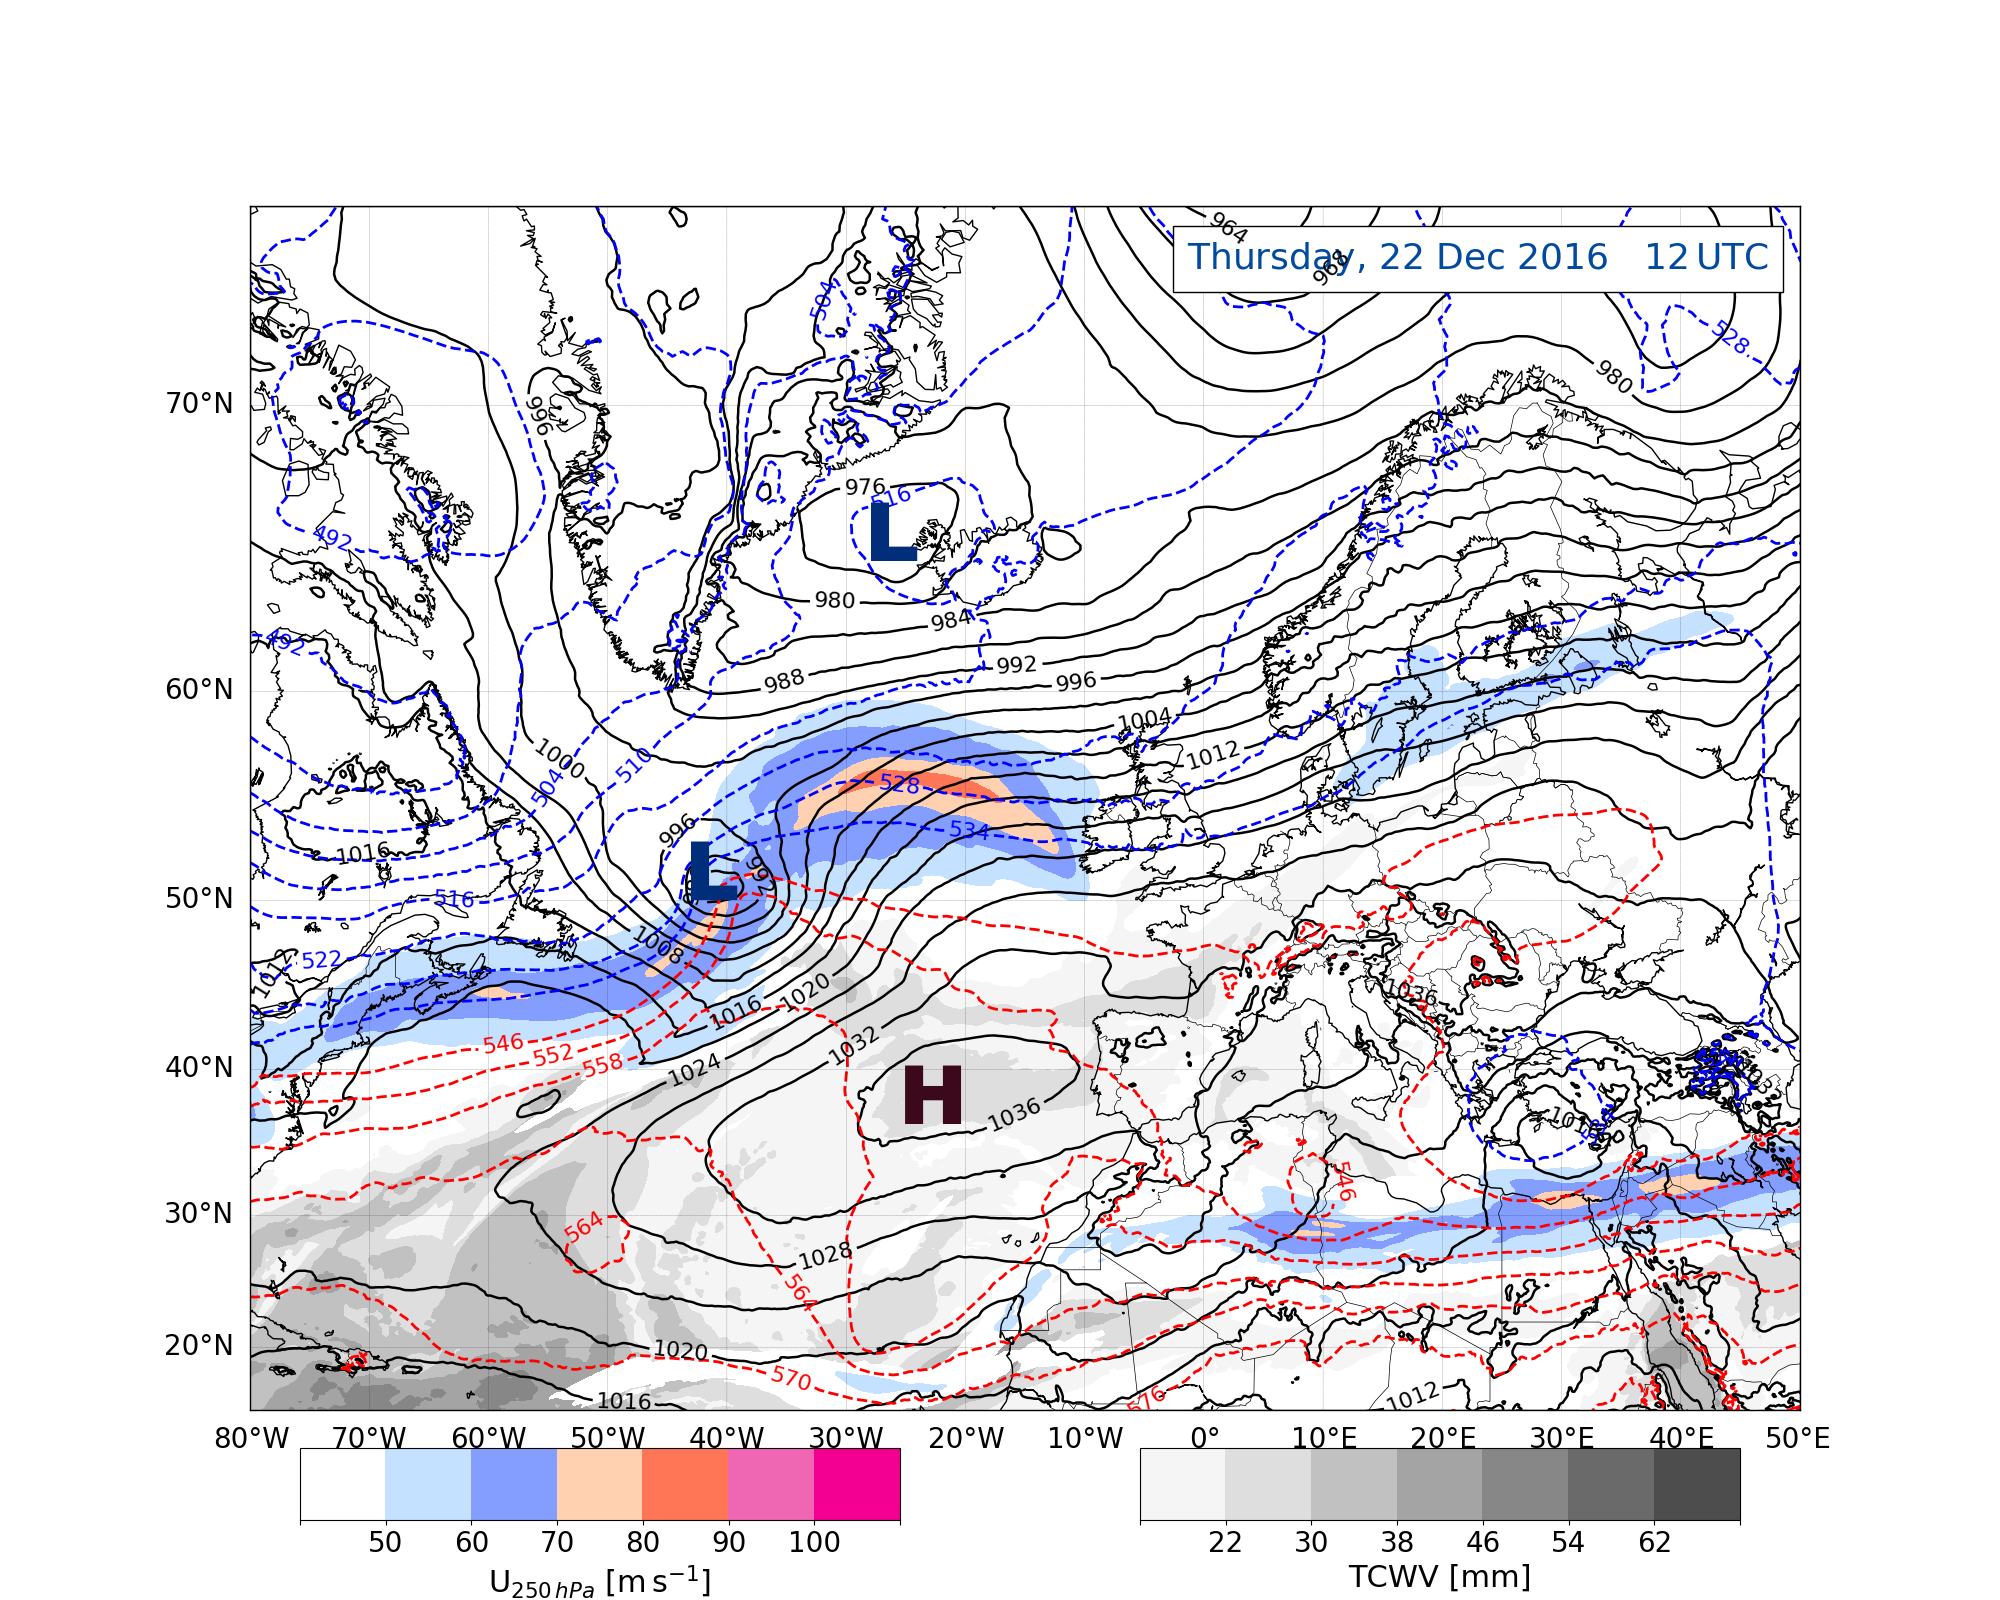
\includegraphics[trim={4.2cm 0cm 4.3cm 5.1cm},clip,
		width=\textwidth]{./fig_Geopot_Jet/20161222_12}
		\caption{} \label{fig:GP22}
	\end{subfigure}
	%     \begin{subfigure}[b]{0.49\textwidth}
	%     	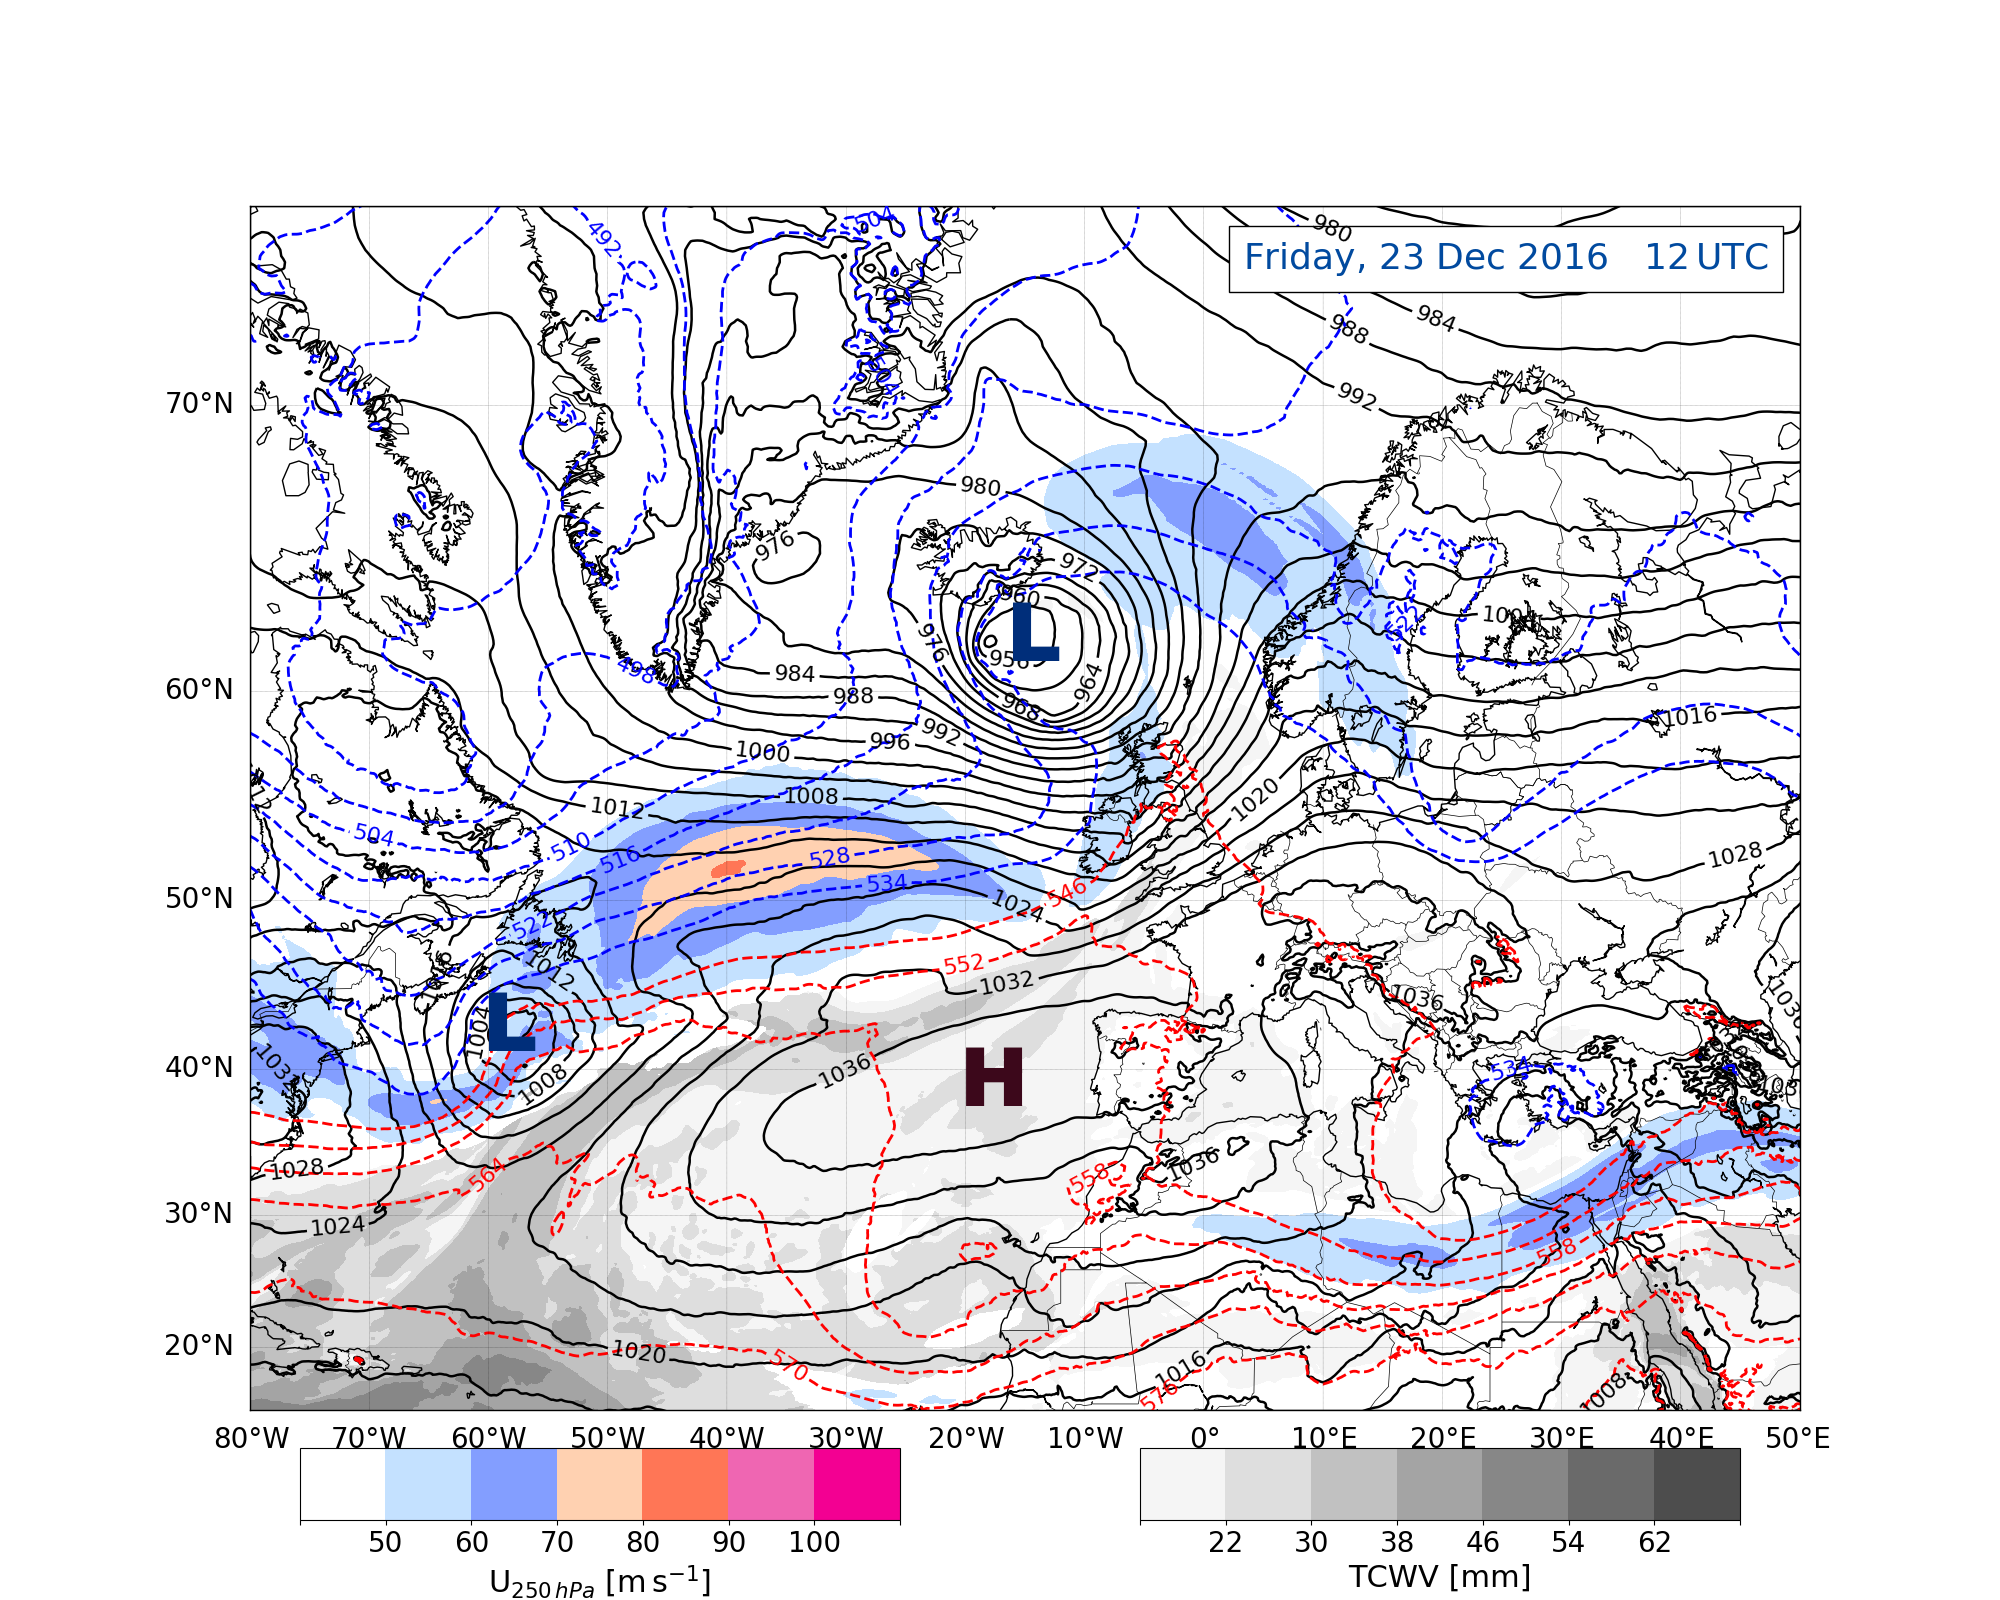
\includegraphics[trim={4.2cm 0cm 4.3cm 5.1cm},clip,
	% 		width=\textwidth]{./fig_Geopot_Jet/20161223_12}
	% 		\caption{} \label{fig:GP23}
	%     \end{subfigure}
	%%% local obs %%%%
	\begin{subfigure}[b]{0.49\textwidth}
		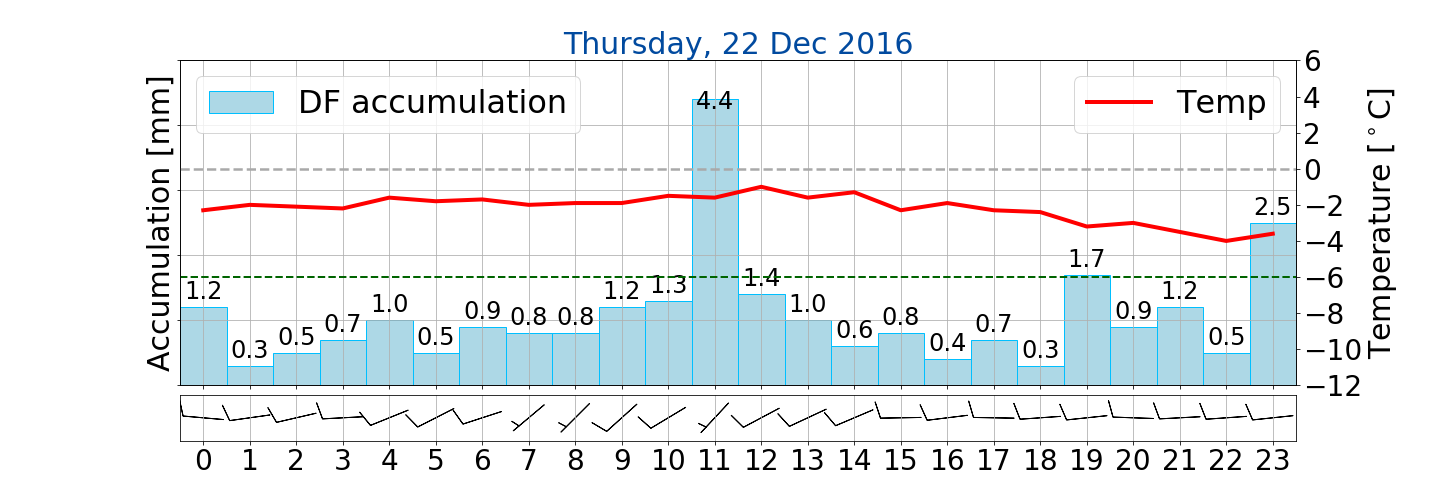
\includegraphics[trim={4.9cm 1.cm 1.5cm 1cm},clip,
		width=\textwidth]{./fig_weathermast/T_P_U_20161222}
		\caption{} \label{fig:TPU22}
	\end{subfigure}
	%     \begin{subfigure}[b]{0.49\textwidth}
	%     	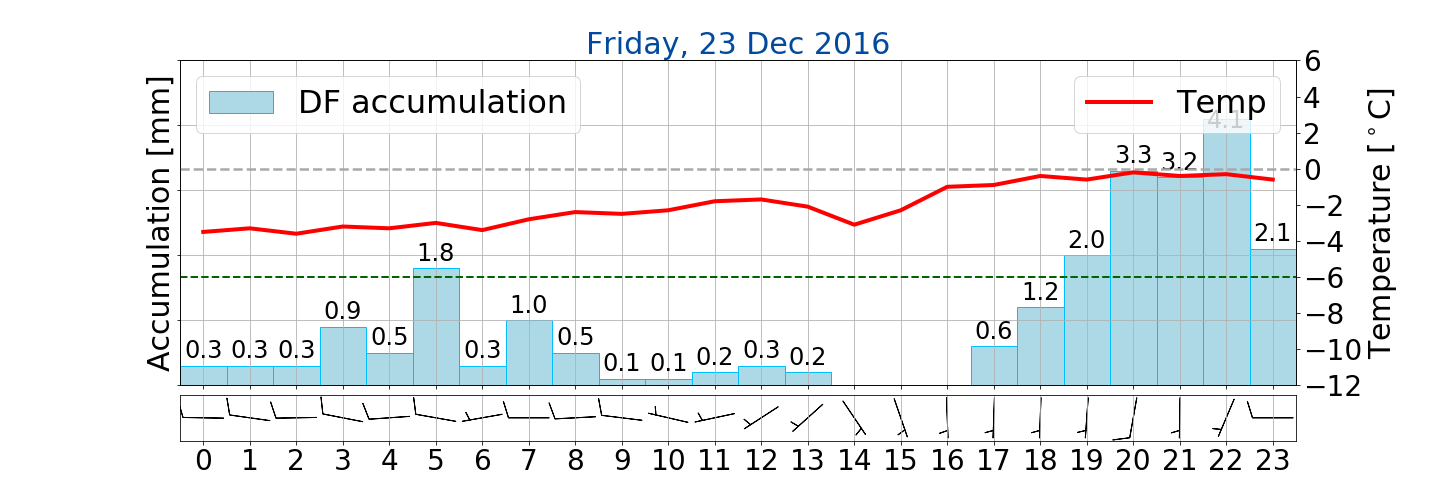
\includegraphics[trim={4.9cm 1.cm 1.5cm 1cm},clip,
	% 		width=\textwidth]{./fig_weathermast/T_P_U_20161223}
	% 		\caption{} \label{fig:TPU23}
	%     \end{subfigure}
\end{figure}
\subsection*{\SI{22}{\dec}}
%%% 22/12
% 22/12
% @ DT, phasing of the vorticity
% → low center is in perfect condition for synoptic scale lifting
\noindent Twenty-four hours later the analysis shows from \SI{22}{\dec} phasing between the surface relative vorticity and the baroclinic zone at \ang{50}{\,N} in the DT. The centre of the surface low is directly located below the temperature gradient at the \SI{2}{PVU} surface, hence this is good for synoptic lifting. Furthermore, the strongest baroclinicity is observed on the south west side of the surface low.
The synoptic map of the geopotential thickness and the surface pressure show the beginning of the frontal boundaries in \Cref{fig:GP22}. 
At the same time shows the AR map, \Cref{fig:AR22}, large values just at the baroclinic zone, where the low pressure is beginning to form. \textcolor{red}{Help?! Does that lead to even more lifting in this area? Or does it just mean that the cyclone gets a good amount of moisture?!}.
Norway is located in a cold area. The continues precipitation observed at Haukeliseter (\Cref{fig:TPU22}) is associated with the westerly flow which is conducive to orographic lifting, and therefore moisture release.  

\begin{figure}
	\centering
	%%% dyntropo %%%%
	\begin{subfigure}[b]{0.49\textwidth}
		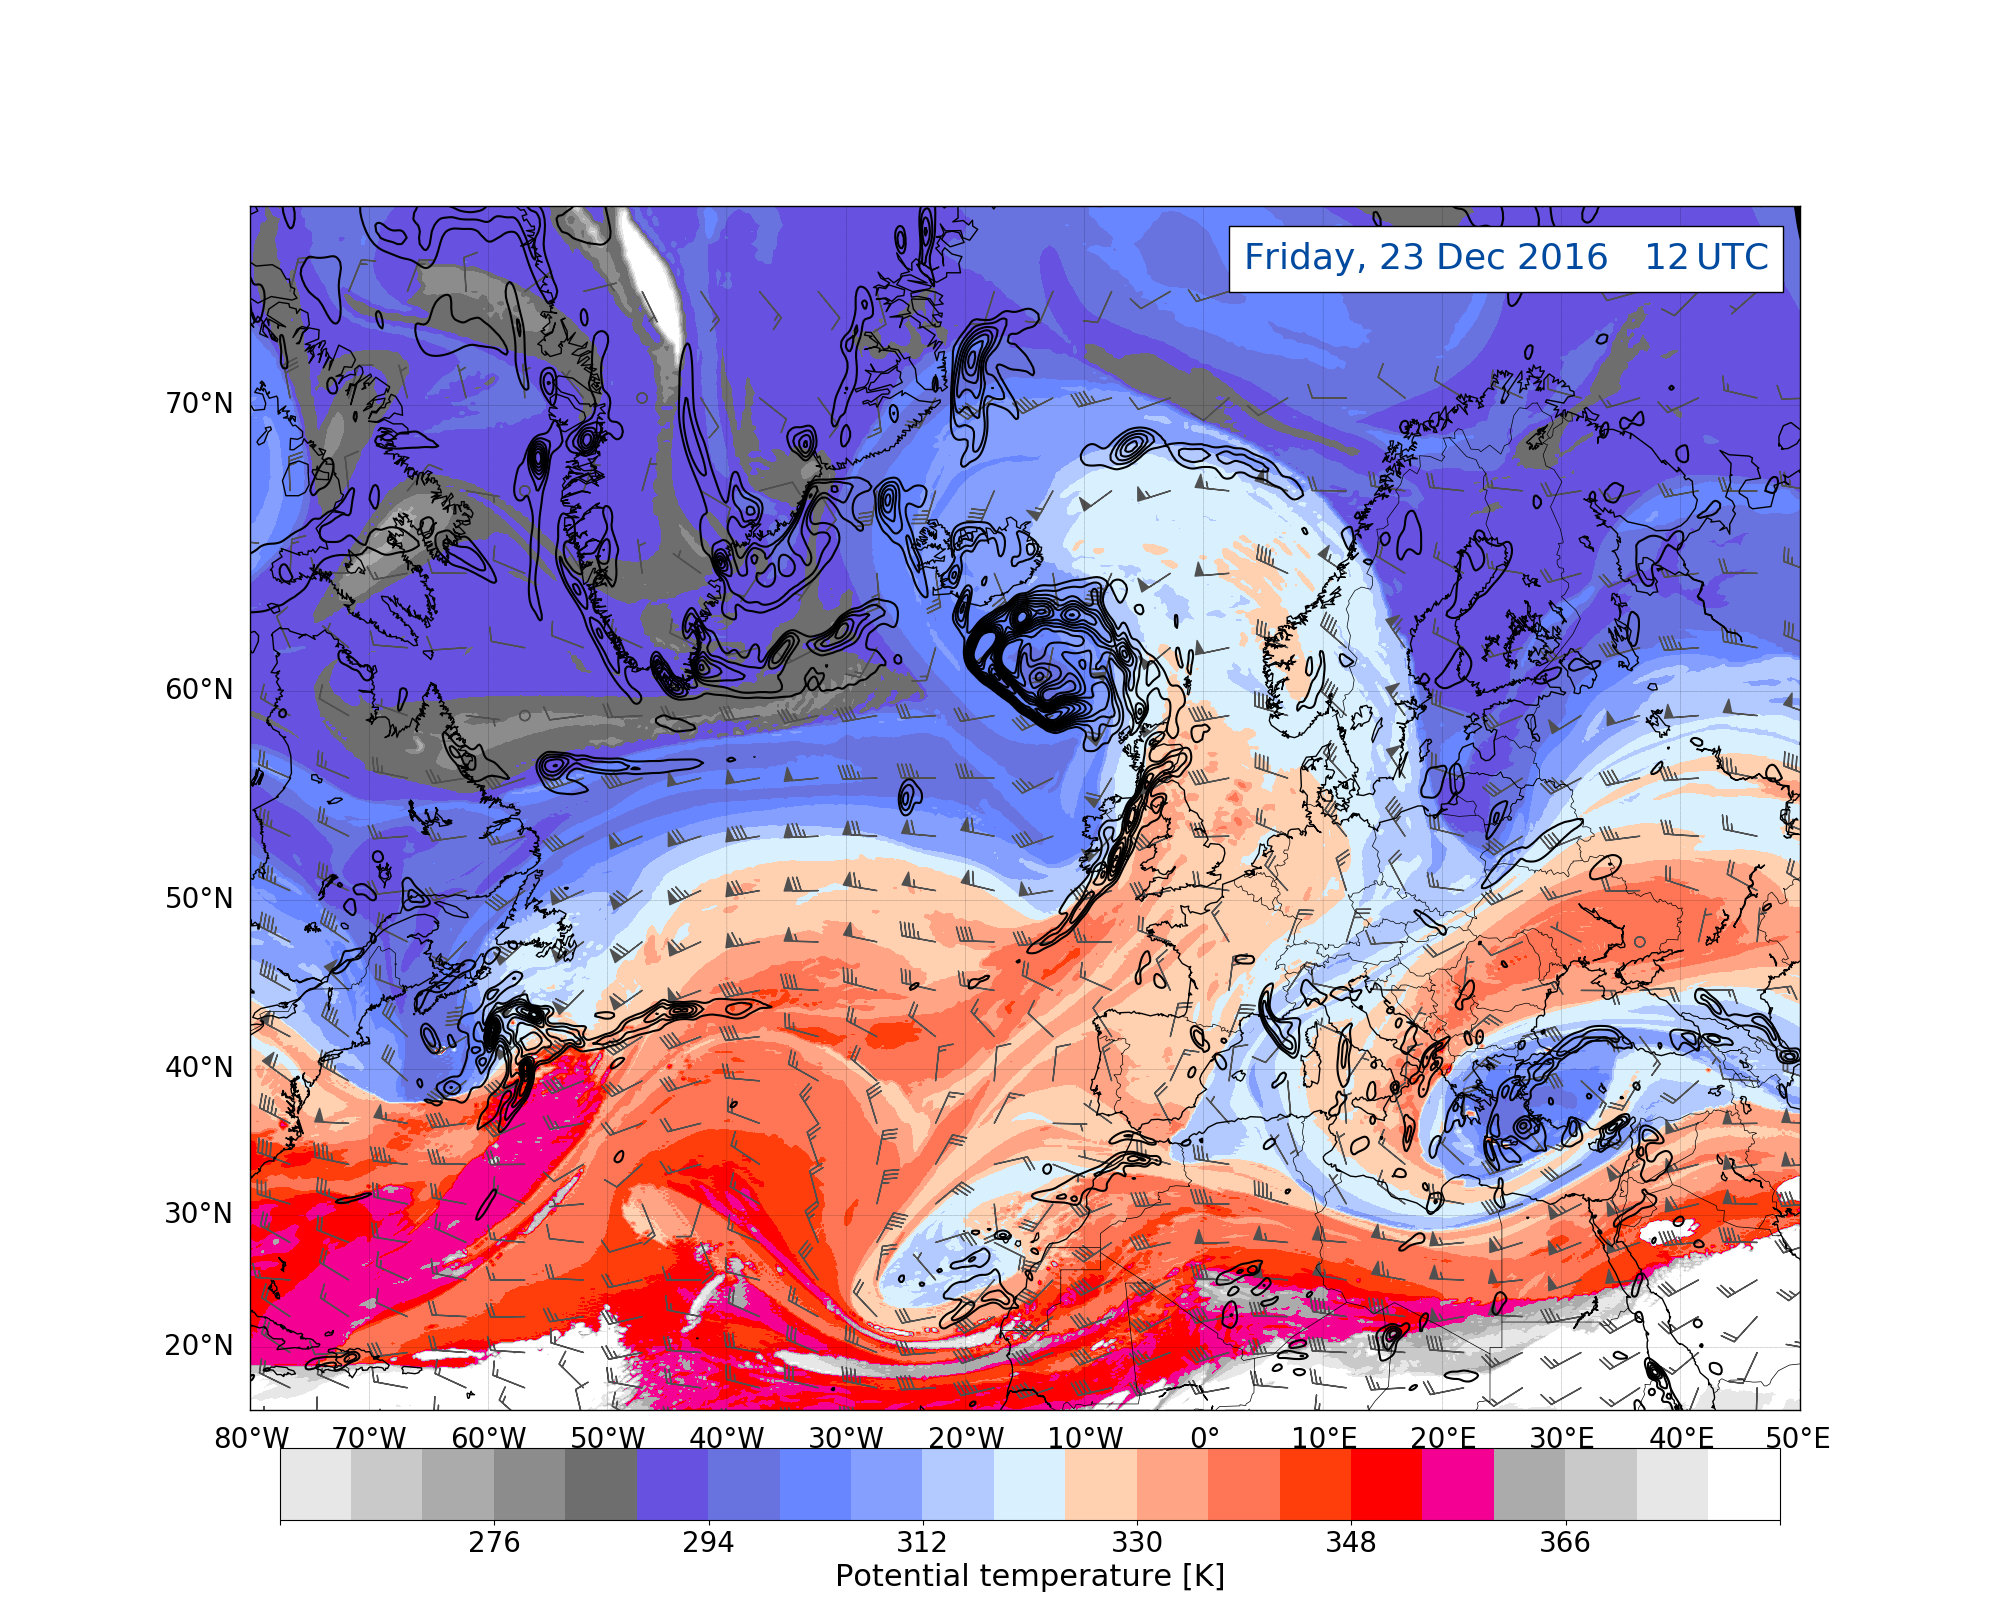
\includegraphics[trim={4.2cm 0cm 4.3cm 5.1cm},clip,
		width=\textwidth]{./fig_DynTropo/20161223_12}
		\caption{} \label{fig:DT23}
	\end{subfigure}
	\begin{subfigure}[b]{0.49\textwidth}
		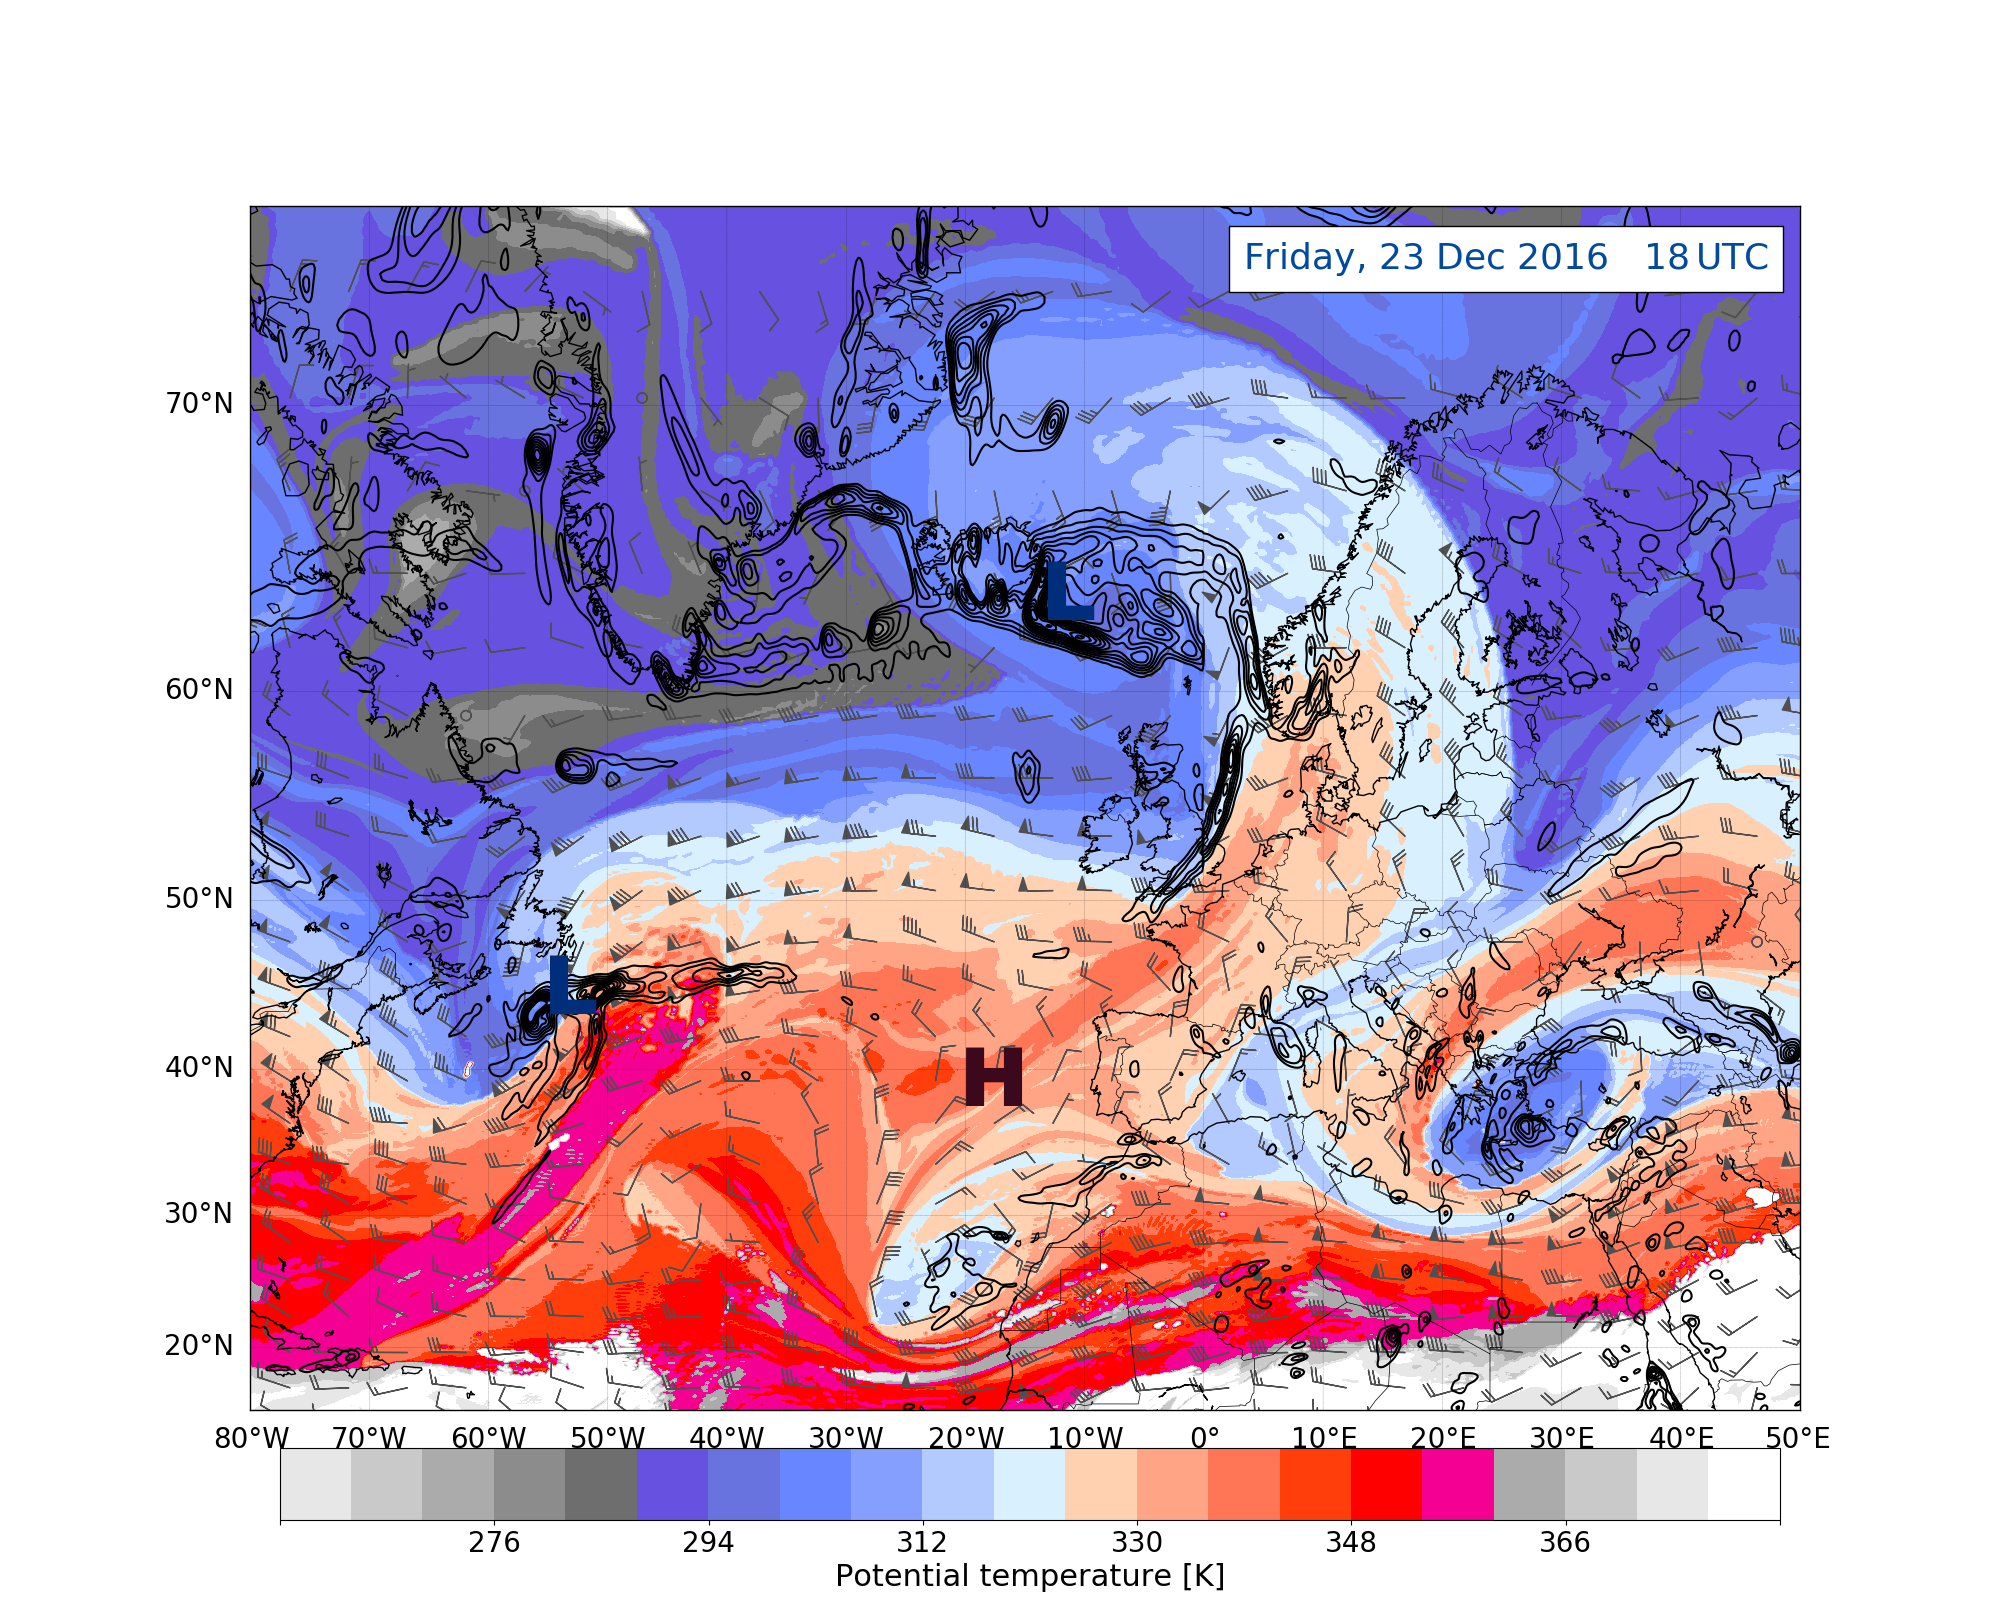
\includegraphics[trim={4.2cm 0cm 4.3cm 5.1cm},clip,
		width=\textwidth]{./fig_DynTropo/20161223_18}
		\caption{} \label{fig:DT23_18}
	\end{subfigure}
	%%% geopot %%%%
	\begin{subfigure}[b]{0.49\textwidth}
		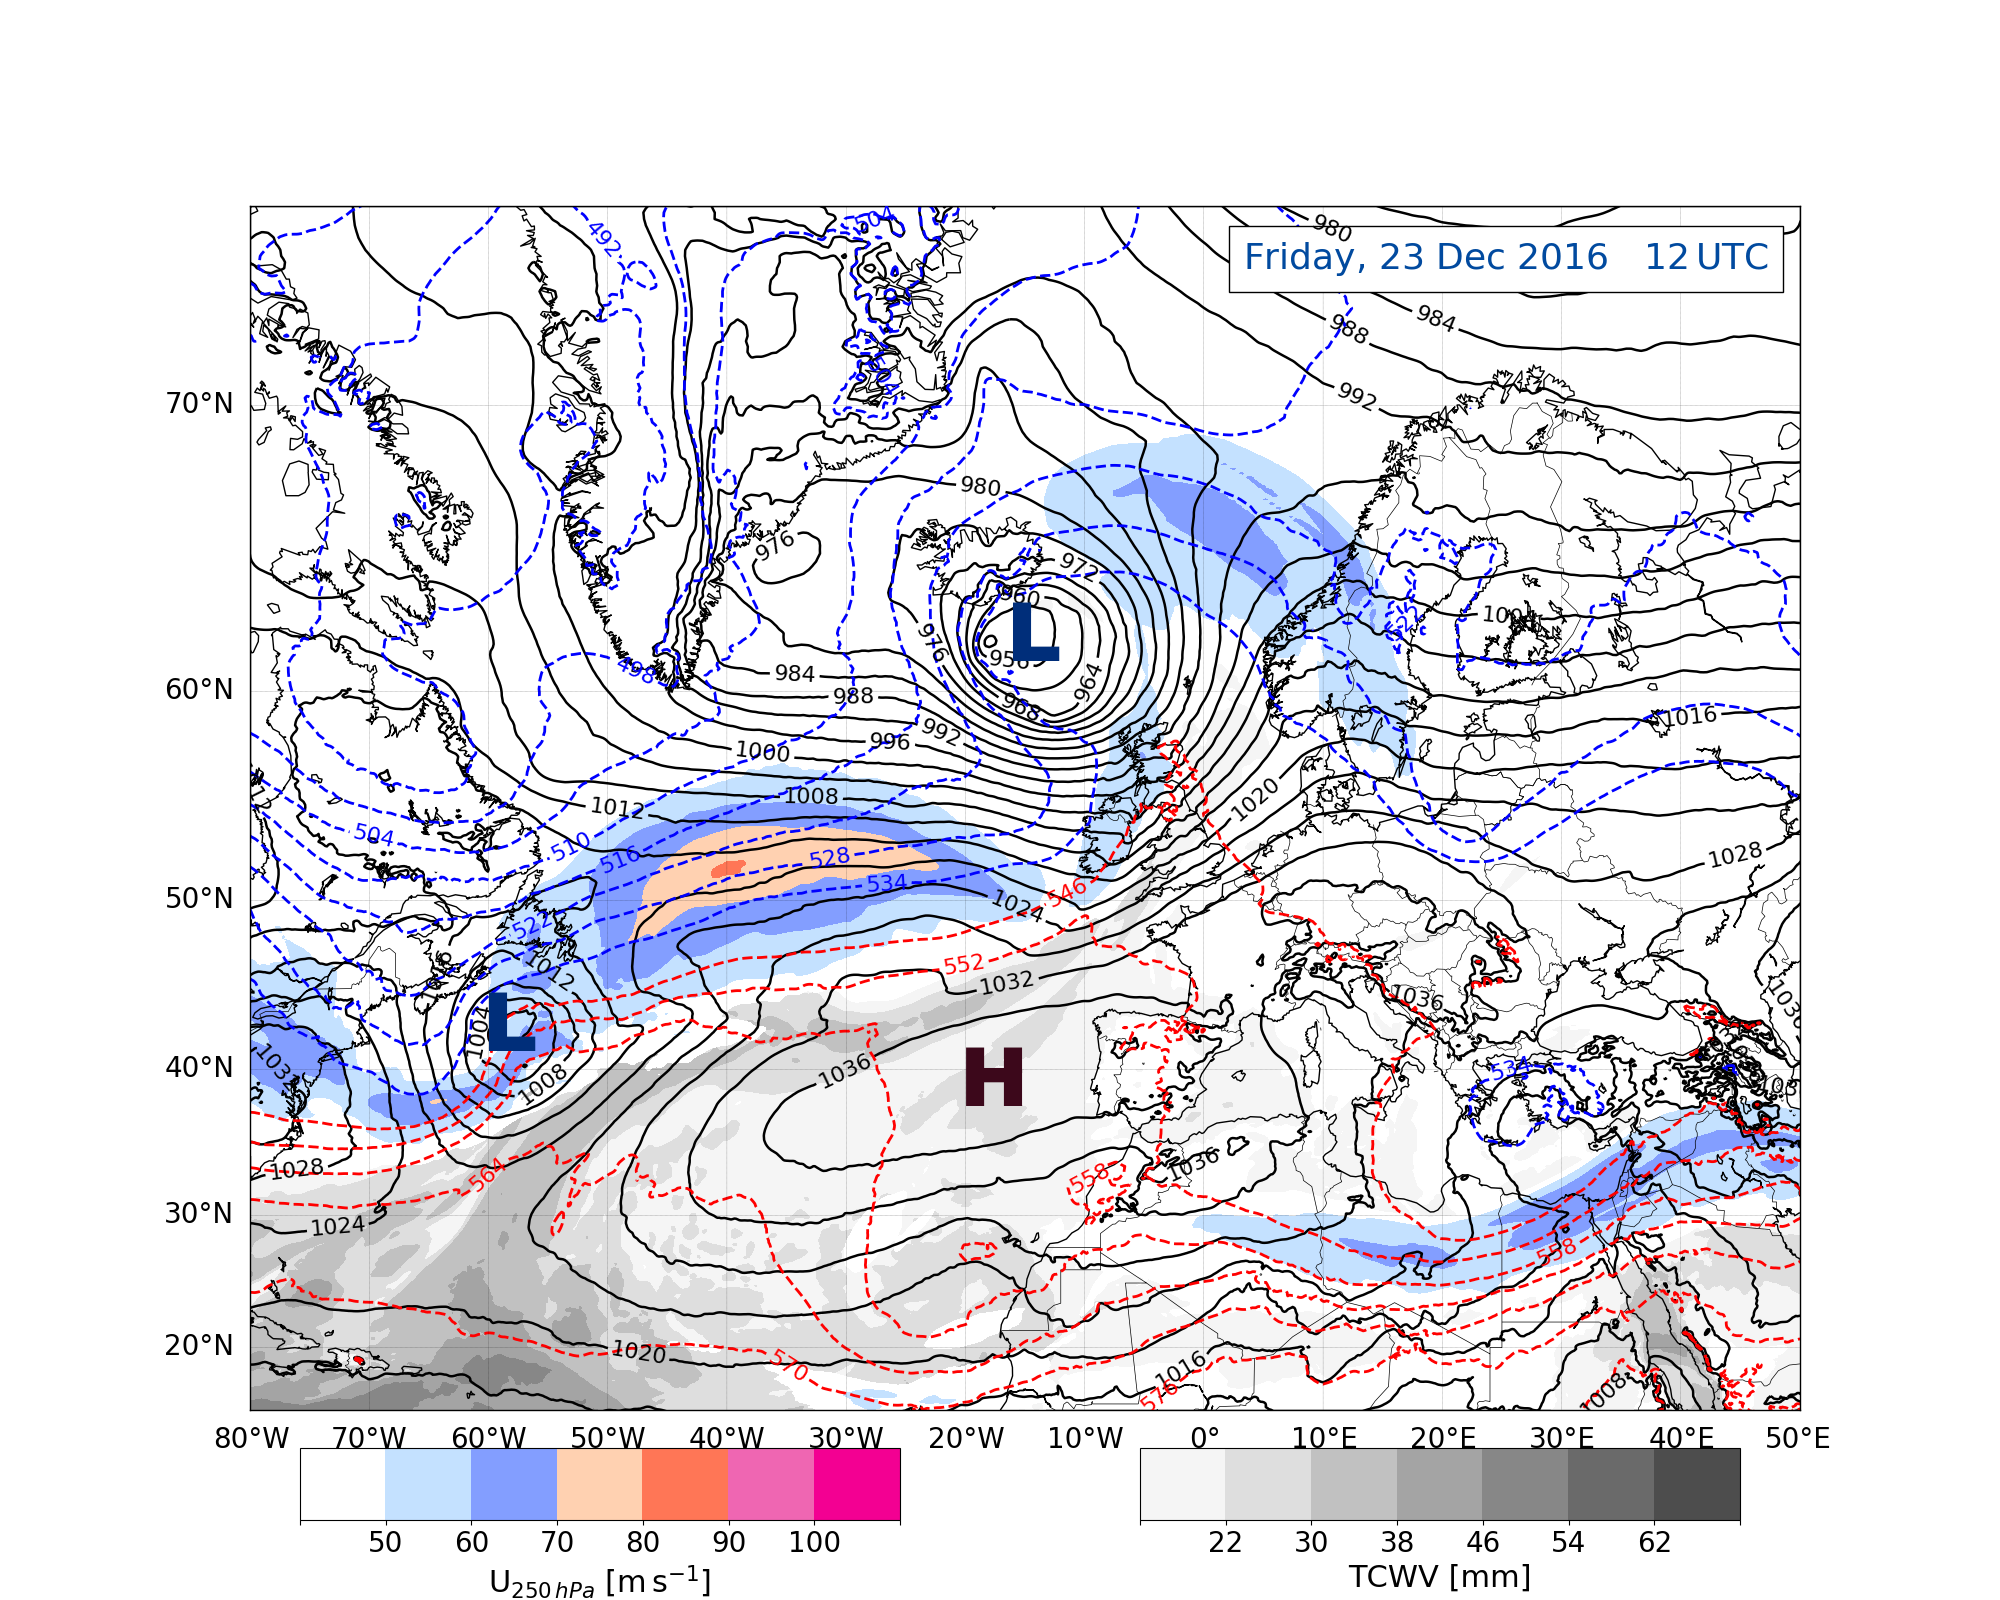
\includegraphics[trim={4.2cm 0cm 4.3cm 5.1cm},clip,
		width=\textwidth]{./fig_Geopot_Jet/20161223_12}
		\caption{} \label{fig:GP23}
	\end{subfigure}
	\begin{subfigure}[b]{0.49\textwidth}
		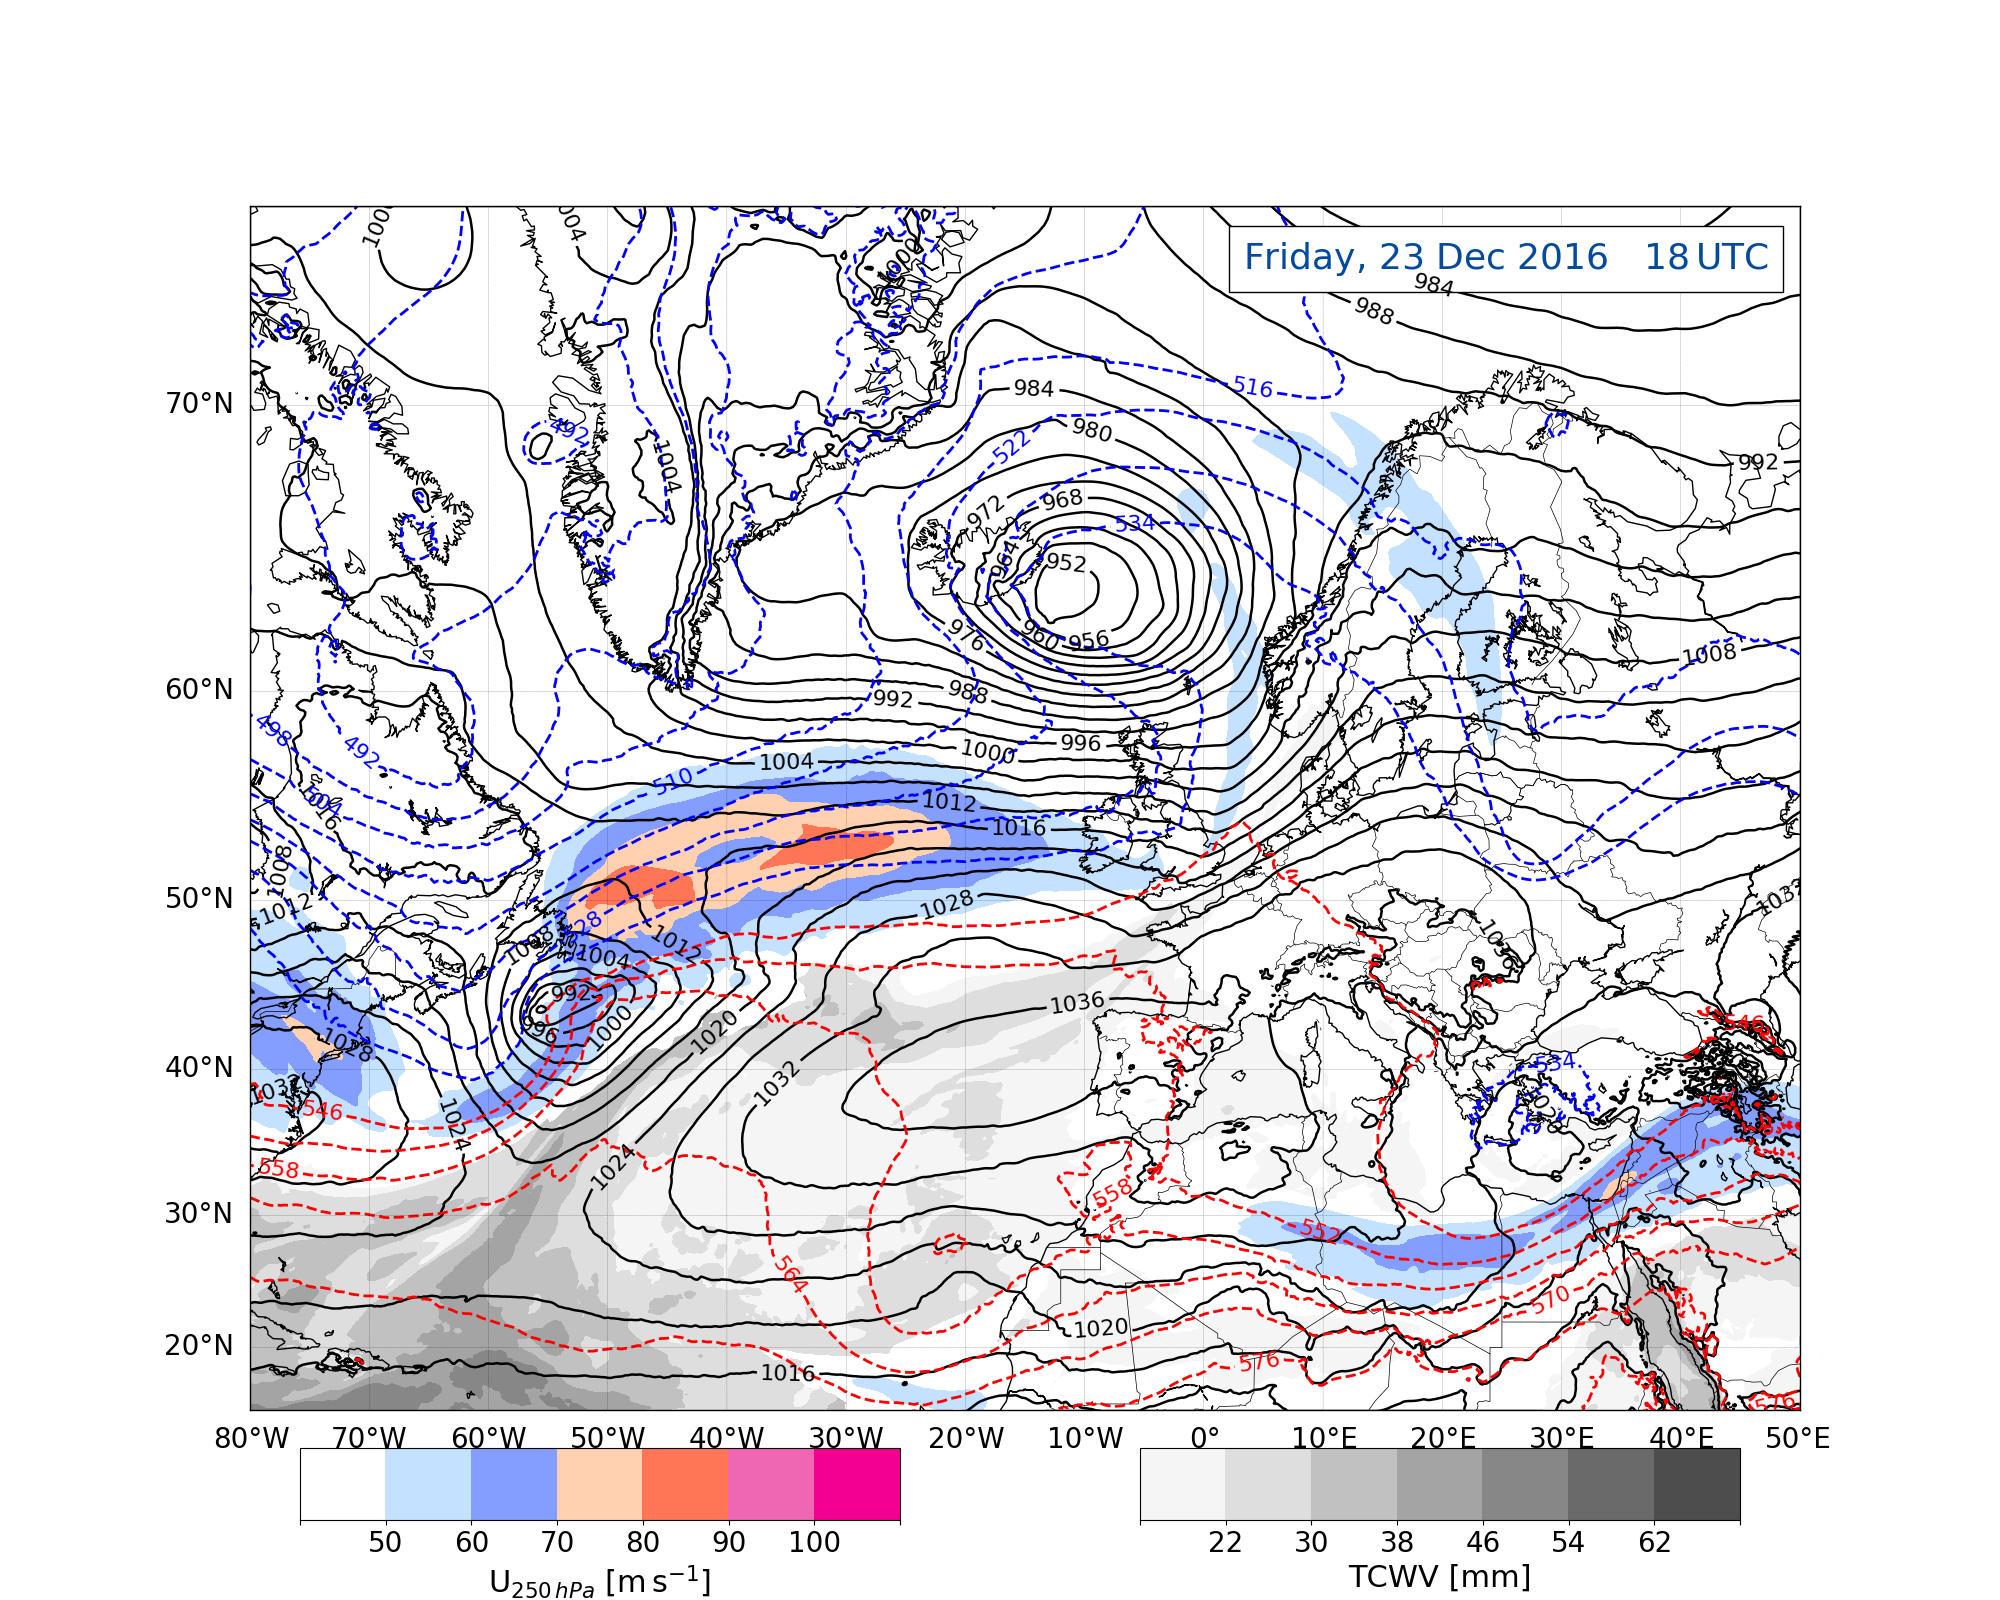
\includegraphics[trim={4.2cm 0cm 4.3cm 5.1cm},clip,
		width=\textwidth]{./fig_Geopot_Jet/20161223_18}
		\caption{} \label{fig:GP23_18}
	\end{subfigure}
	%%% local obs %%%%
	\begin{subfigure}[b]{0.49\textwidth}
		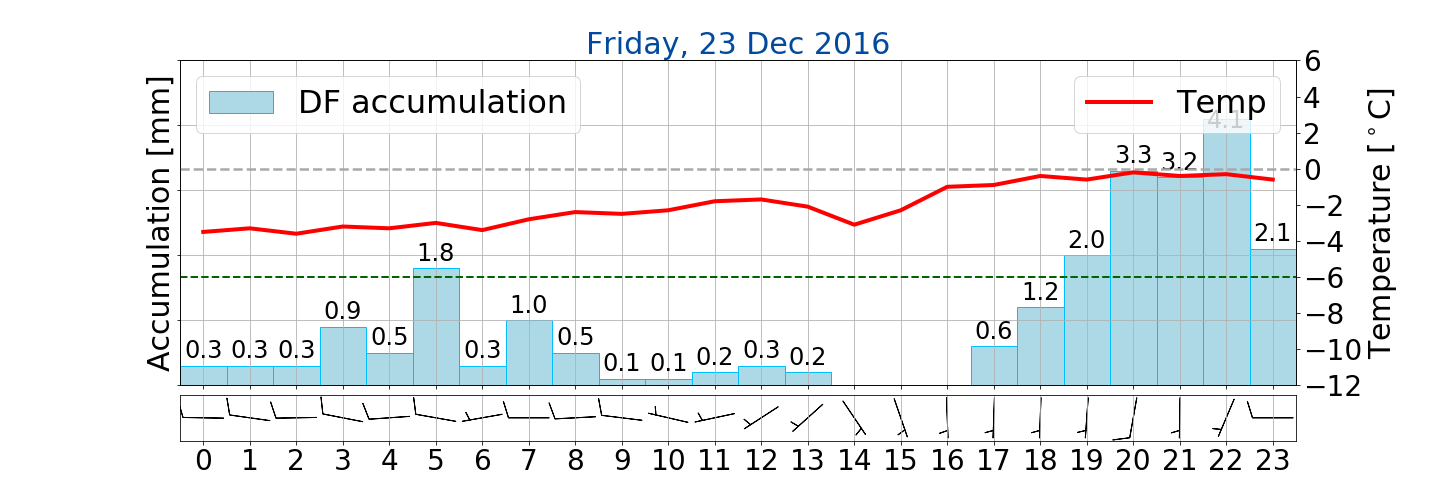
\includegraphics[trim={4.9cm 1.cm 1.5cm 1cm},clip,
		width=\textwidth]{./fig_weathermast/T_P_U_20161223}
		\caption{} \label{fig:TPU23}
	\end{subfigure}
\end{figure}
\subsection*{\SI{23}{\dec}}
%%% 23/12
% 23/06
% Still conducive westerly flow → orographic lifting
% Norway in cold area
% Jet not very strong
% Probably frozen precipitation
% Baroclinicity strongest South West of low center
% Low has well-formed frontal boundaries (low level vorticity, → lifting at the cold frontal boundary?)
% 23/12
% Westerlies change
% That is because of the ridging @ DT
% → pushes away the cold air
% First frontal boundary (warm front/Occluded front?) goes through
% 23/18
% Frontal boundary went through, warms up → probably mixed phase/liquid precip.
% Lifting associates with the warm front
% Some forcing due to low level flow / weak warm front
% Southern Norway is briefly into warm air mass, before the cold front comes along
\textcolor{red}{Use the 12UTC and 18UTC analysis}
\noindent The begin of the ridging on the \SI{22}{\dec} is more pronounced \SI{24}{\hour} later. The warmer air pushes away the cold air, which covered Norway.
The low-pressure system moved north-east and lies south of Iceland. The occluded front of this system passes through Haukeliseter, which is why a temperature 'jump' observed at \SI{14}{\UTC}. After this, Southern Norway is influenced by the warm sector, monitored as a temperature increase. 
The AR, as well as the total column water vapour amount in \Cref{fig:AR23} and \Cref{fig:GP23}, respectively show the amount of moisture, transported from low latitudes.
\\
At the same time forms a second cyclone at the baroclinic zone at \ang{40}{\,N}. The atmospheric river map (\Cref{fig:AR23}) indicates a large amount of moisture at this latitude. Again, moist, warm air is conducive to intensify the surface cyclone. In addition, shows the DT map a phasing between the low-level vorticity and the upper level baroclinic zone. 

\begin{figure}
	\centering
	%%% dyntropo %%%%
	\begin{subfigure}[b]{0.49\textwidth}
		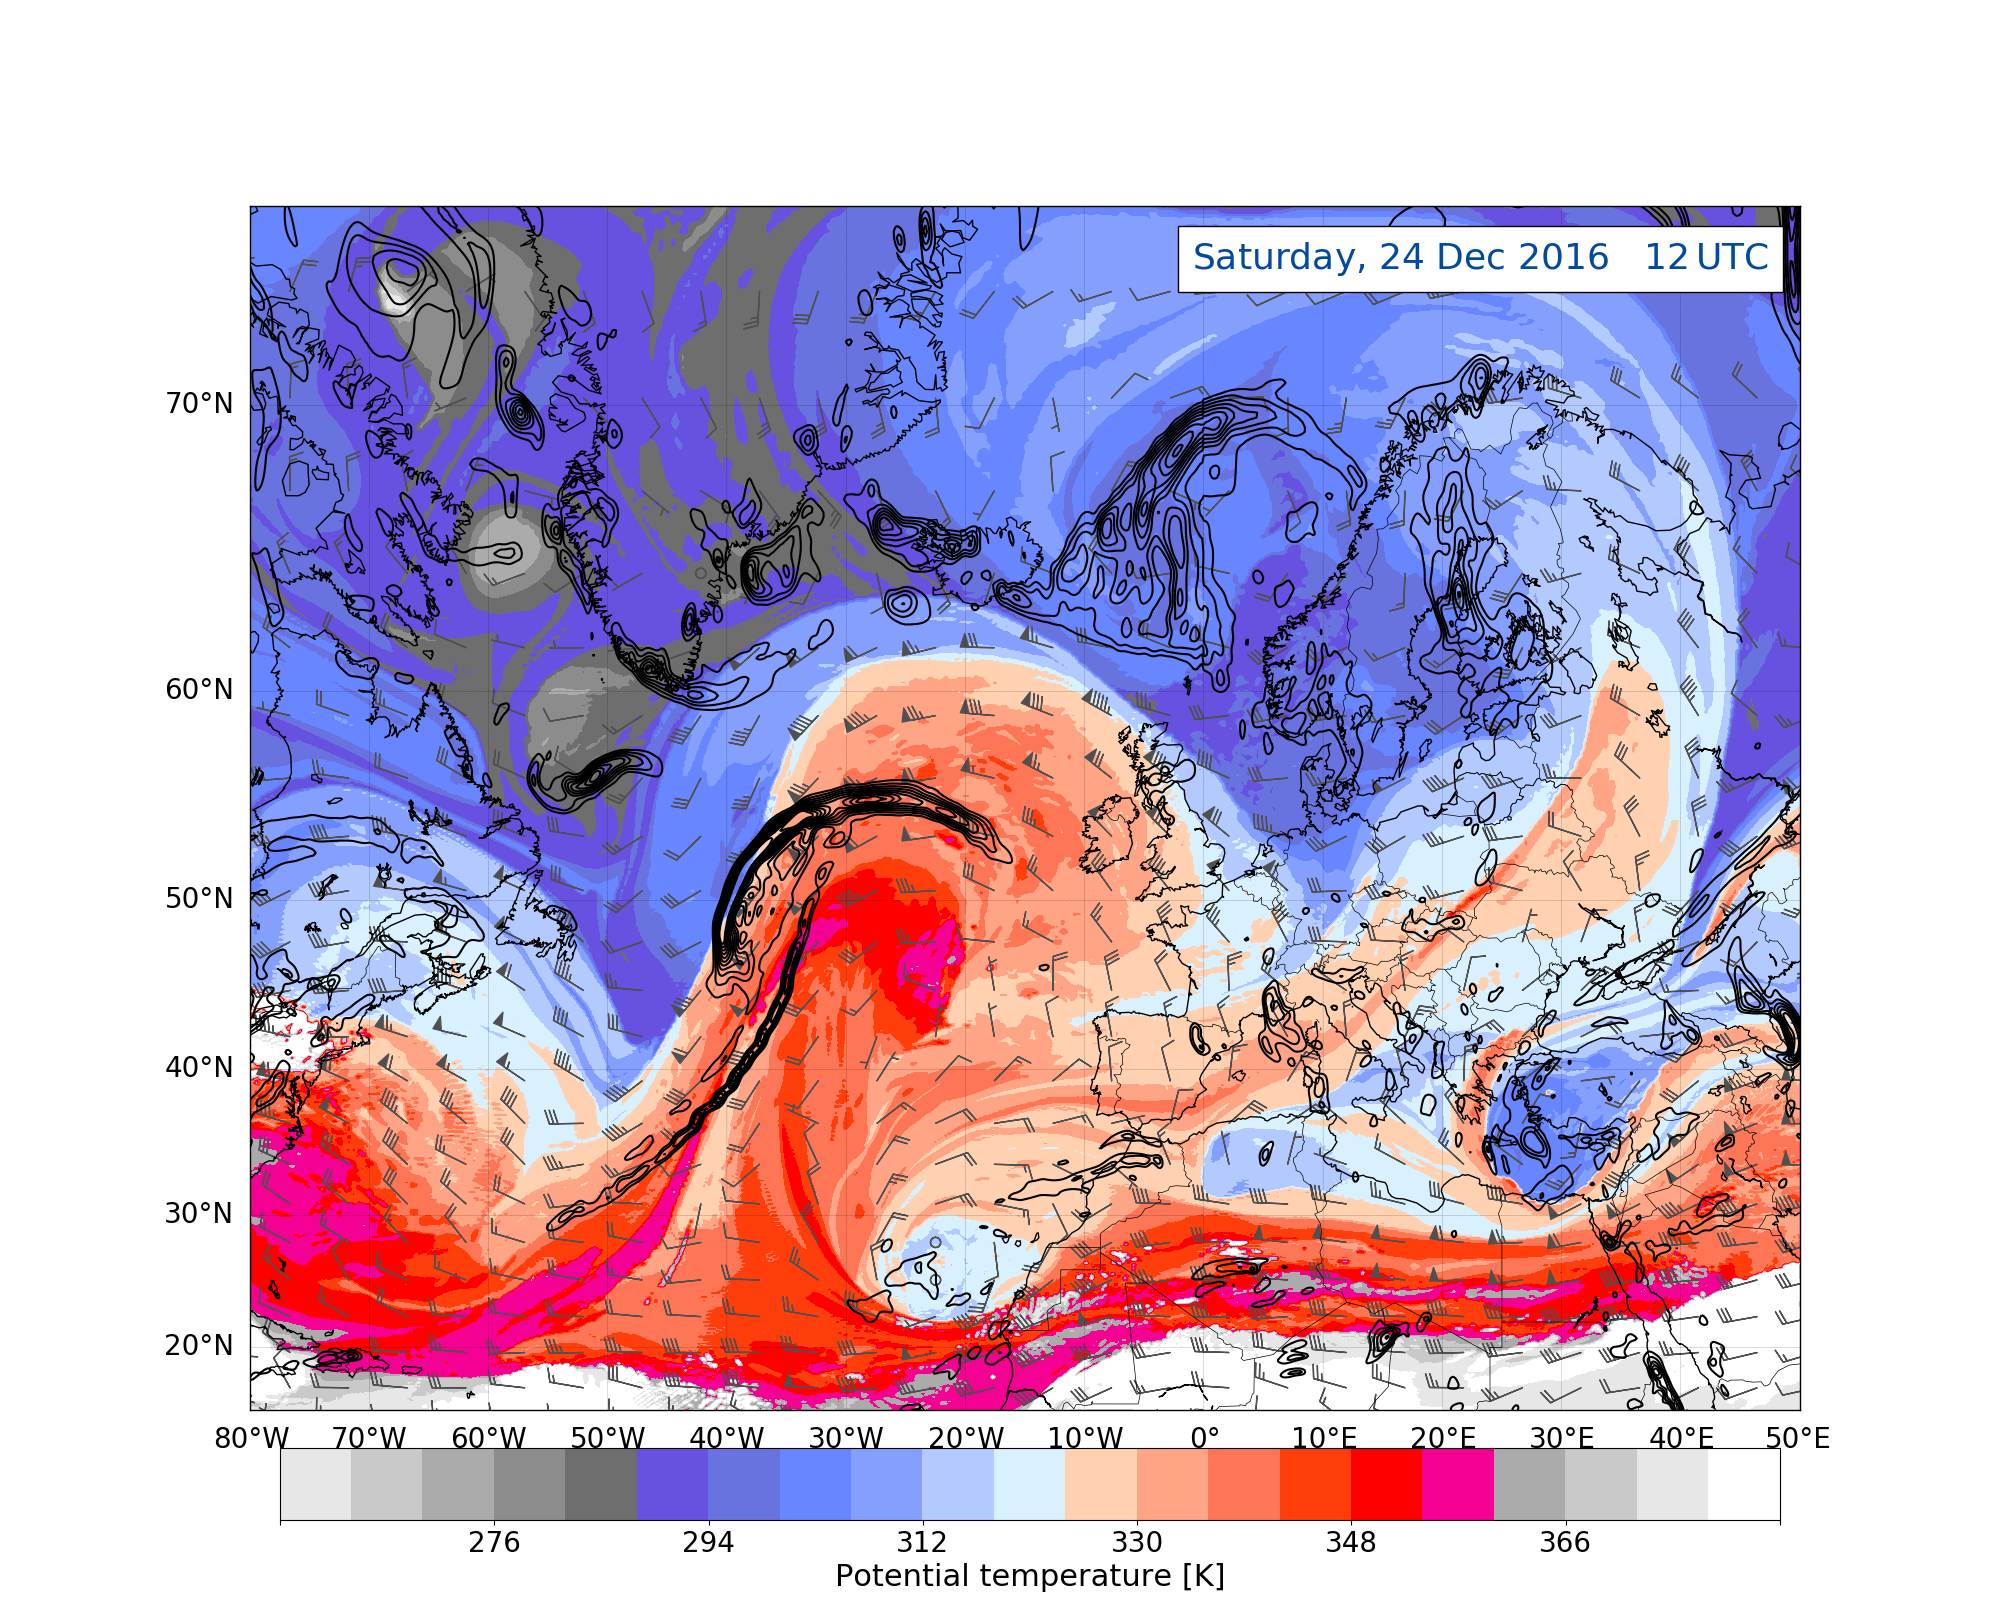
\includegraphics[trim={4.2cm 0cm 4.3cm 5.1cm},clip,
		width=\textwidth]{./fig_DynTropo/20161224_12}
		\caption{} \label{fig:DT24}
	\end{subfigure}
	%%% geopot %%%%
	\begin{subfigure}[b]{0.49\textwidth}
		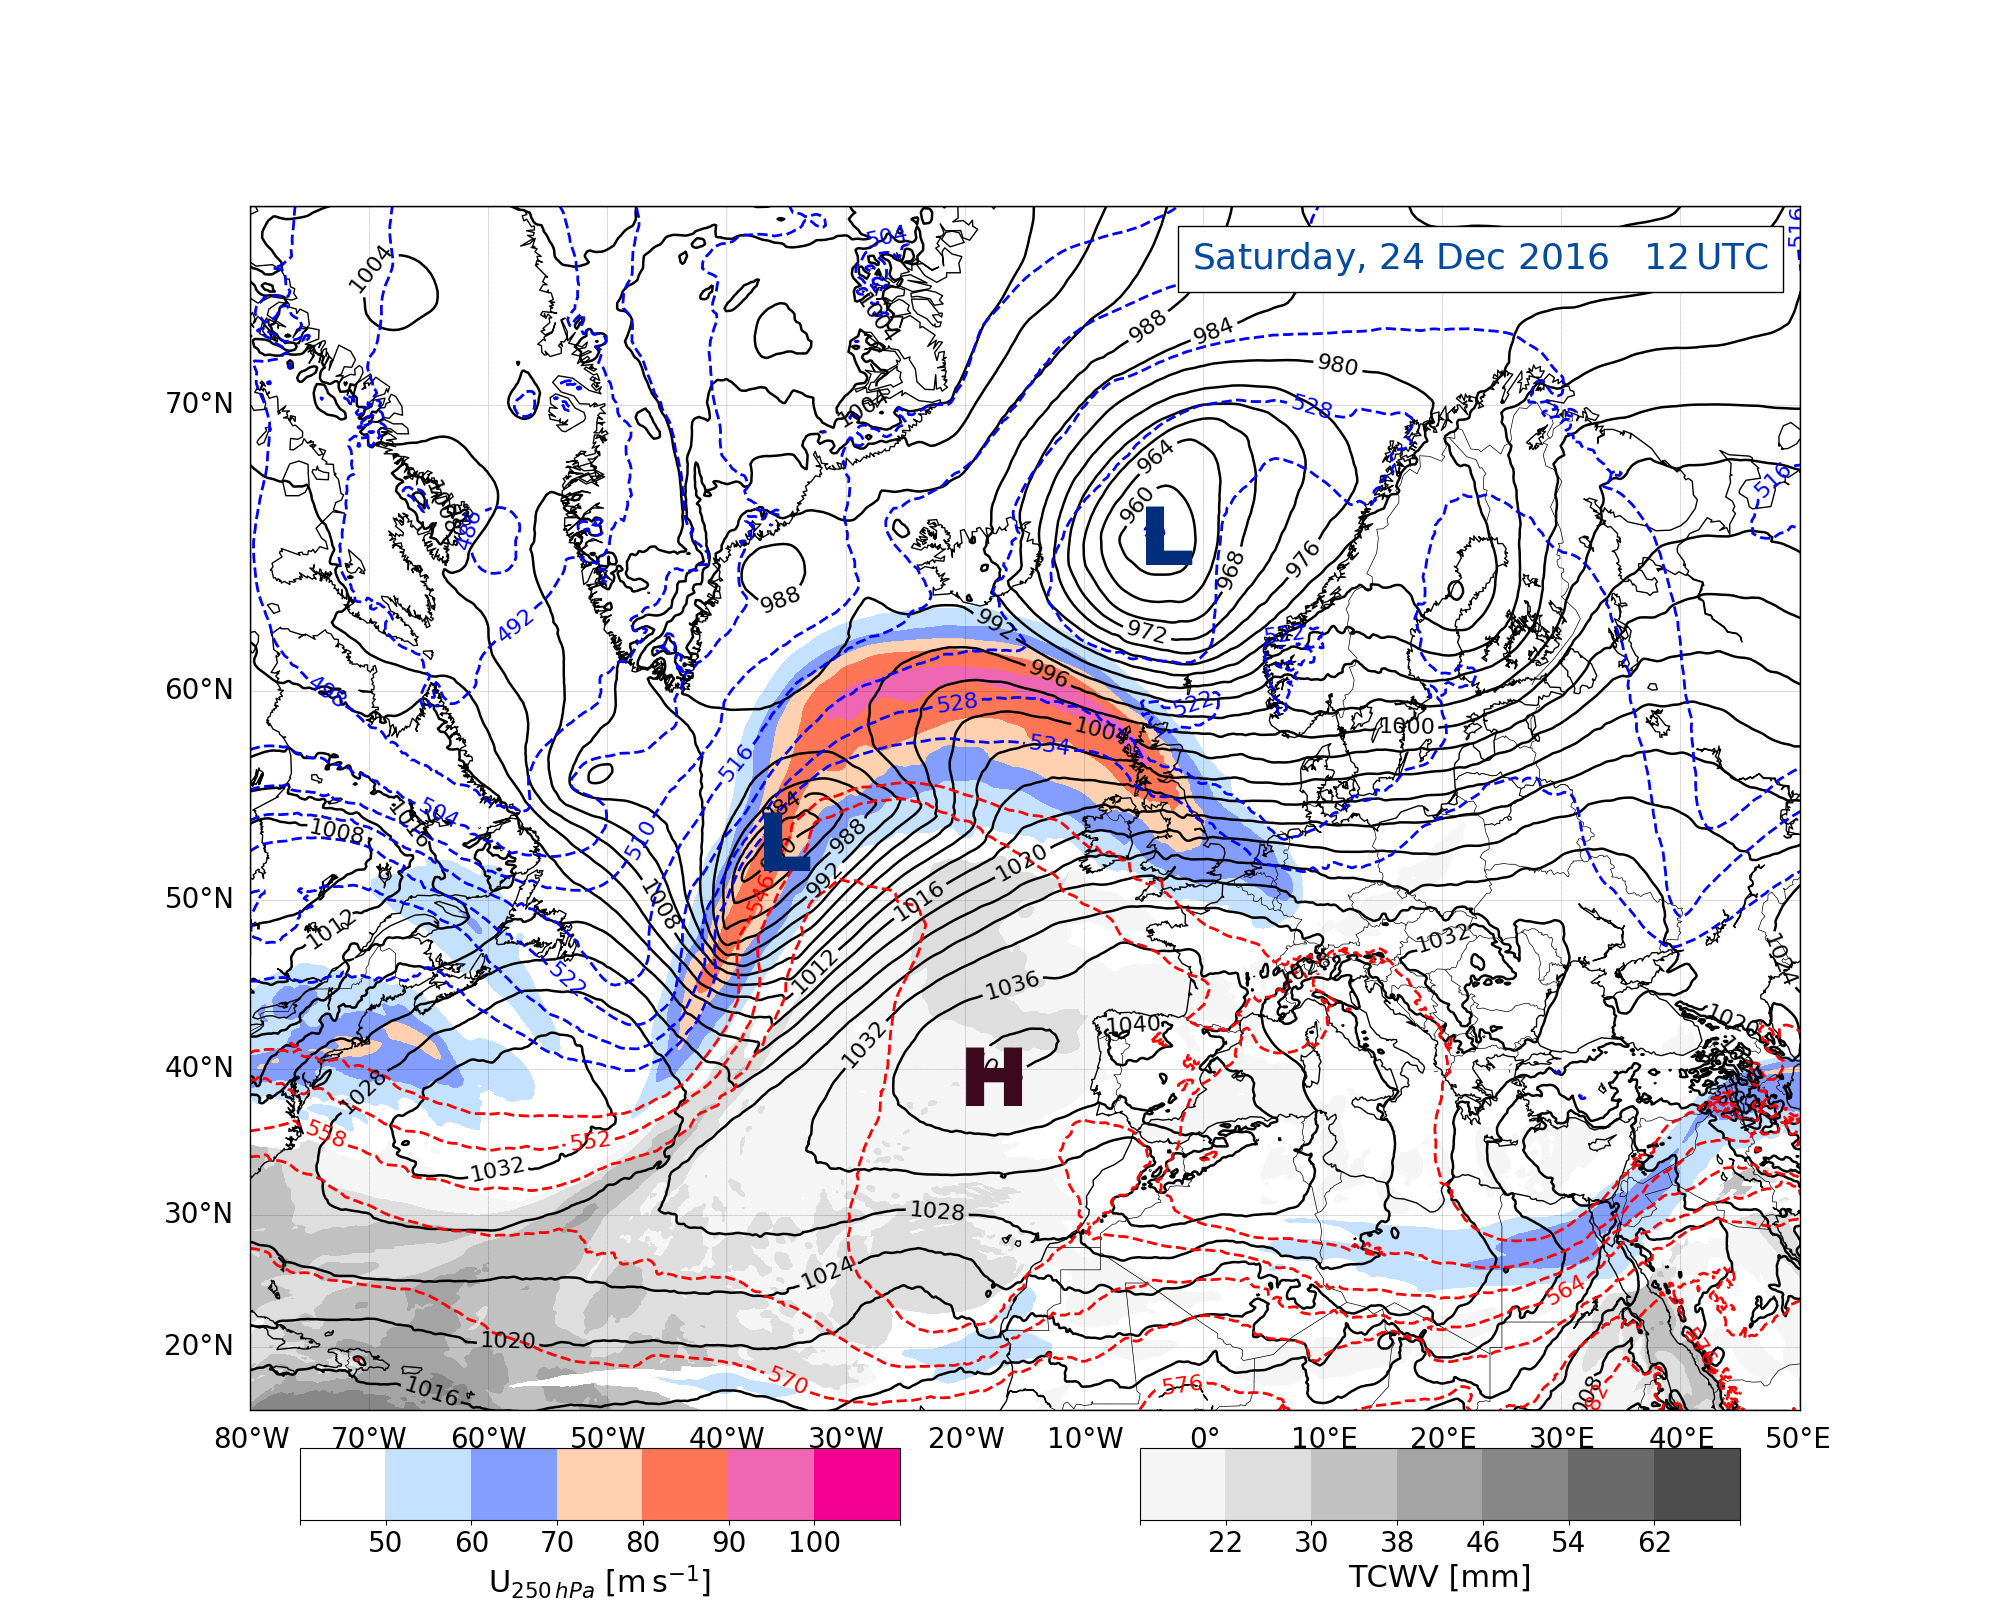
\includegraphics[trim={4.2cm 0cm 4.3cm 5.1cm},clip,
		width=\textwidth]{./fig_Geopot_Jet/20161224_12}
		\caption{} \label{fig:GP24}
	\end{subfigure}
	%%% local obs %%%%
	\begin{subfigure}[b]{0.49\textwidth}
		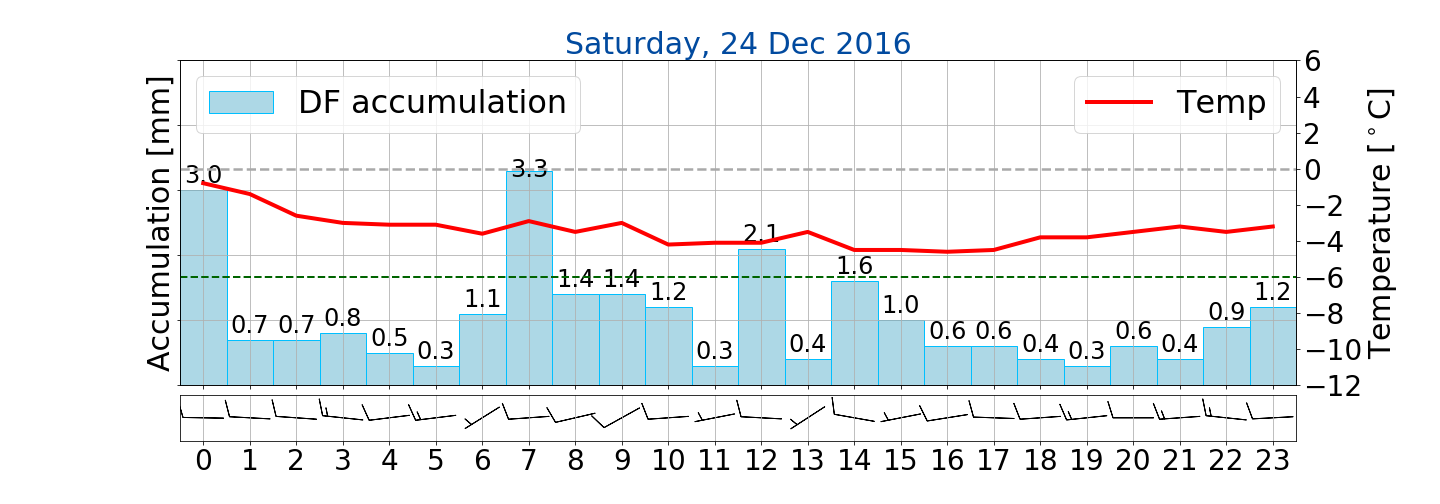
\includegraphics[trim={4.9cm 1.cm 1.5cm 1cm},clip,
		width=\textwidth]{./fig_weathermast/T_P_U_20161224}
		\caption{} \label{fig:TPU24}
	\end{subfigure}
\end{figure}
\subsection*{\SI{24}{\dec}}
%%% 24/12
% 24/00
% Norway goes right back into colder air @ DT, @ sfc (thickness lines)
% @ DT lifting associated with the low-level vorticity 
% 24/12
% Cold frontal boundary pushes through
% Norway is back into colder air → reduction in temp.
% Again, westerly flow → good for orographic lifting
\noindent After the passage of the cold front over Norway, Scandinavia is within colder air (compare \Cref{fig:DT24} and \Cref{fig:GP24} for \SI{24}{\dec}). Over the Atlantic warmer air starts to push the colder air northward. \textcolor{red}{something something with the low-level vorticity and lifting; lifting at the right entrance region of the jet streak, and very high IVT}.
\\
At Haukeliseter negative temperature up to \SI{-4}{\celsius} is observed, compare \Cref{fig:TPU24}. The westerly flow is again conducive for orographic lifting and associated precipitation.

\begin{figure}
	\centering
	%%% dyntropo %%%%
	\begin{subfigure}[b]{0.49\textwidth}
		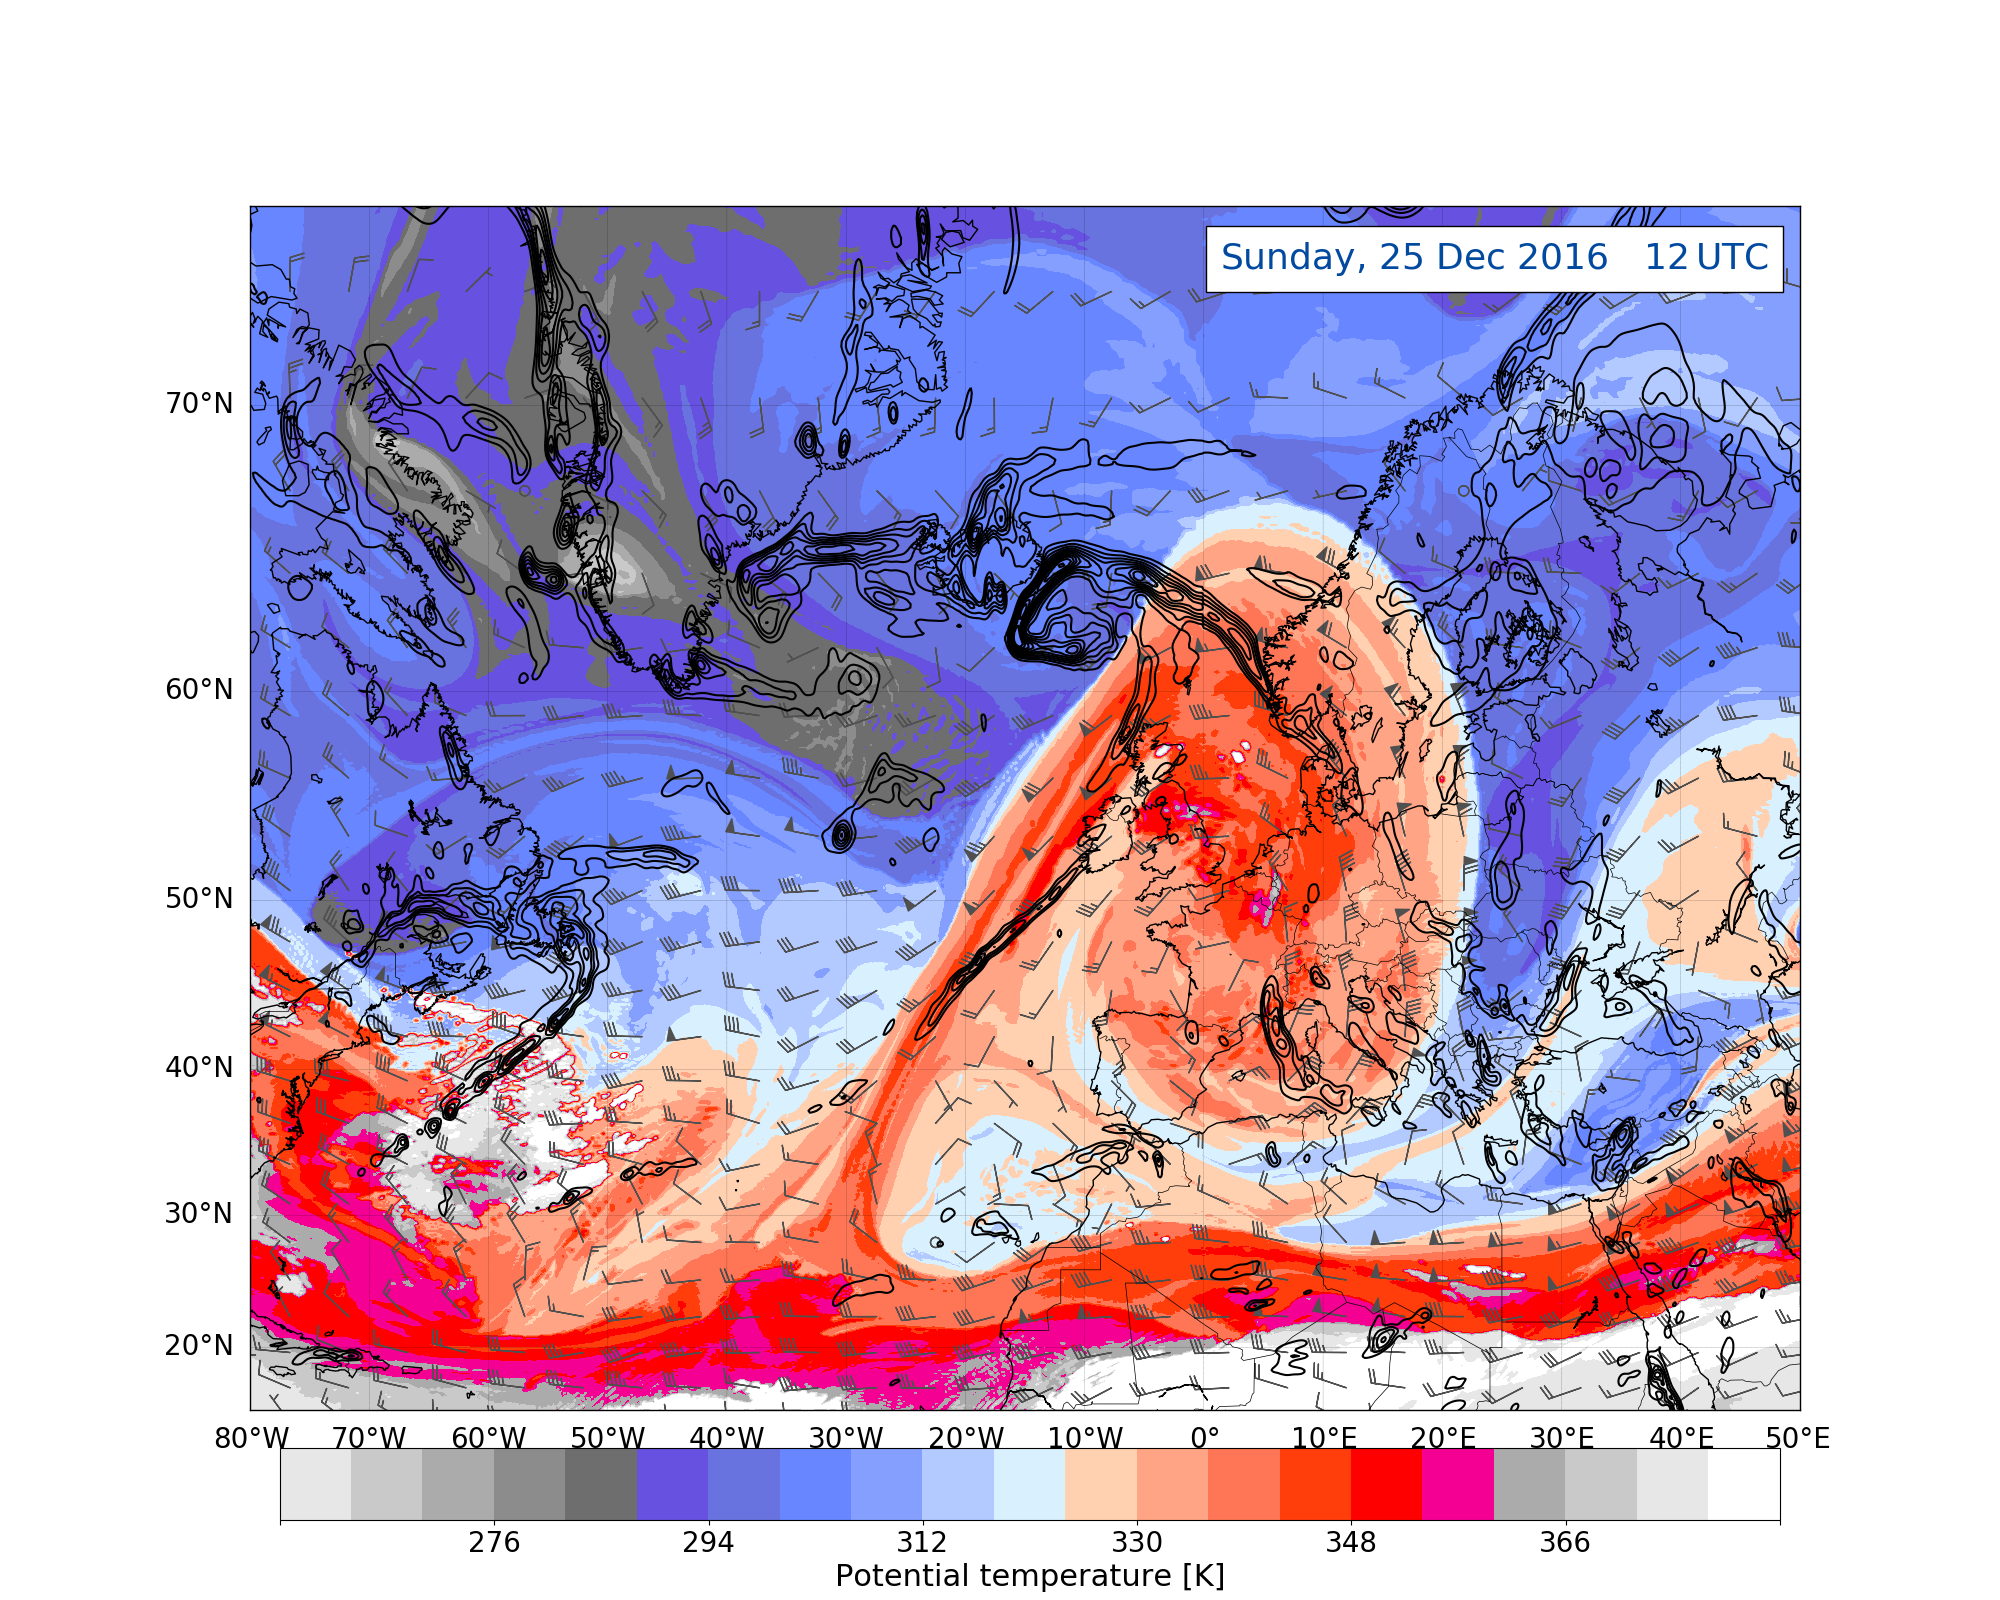
\includegraphics[trim={4.2cm 0cm 4.3cm 5.1cm},clip,
		width=\textwidth]{./fig_DynTropo/20161225_12}
		\caption{} \label{fig:DT25}
	\end{subfigure}
	\begin{subfigure}[b]{0.49\textwidth}
		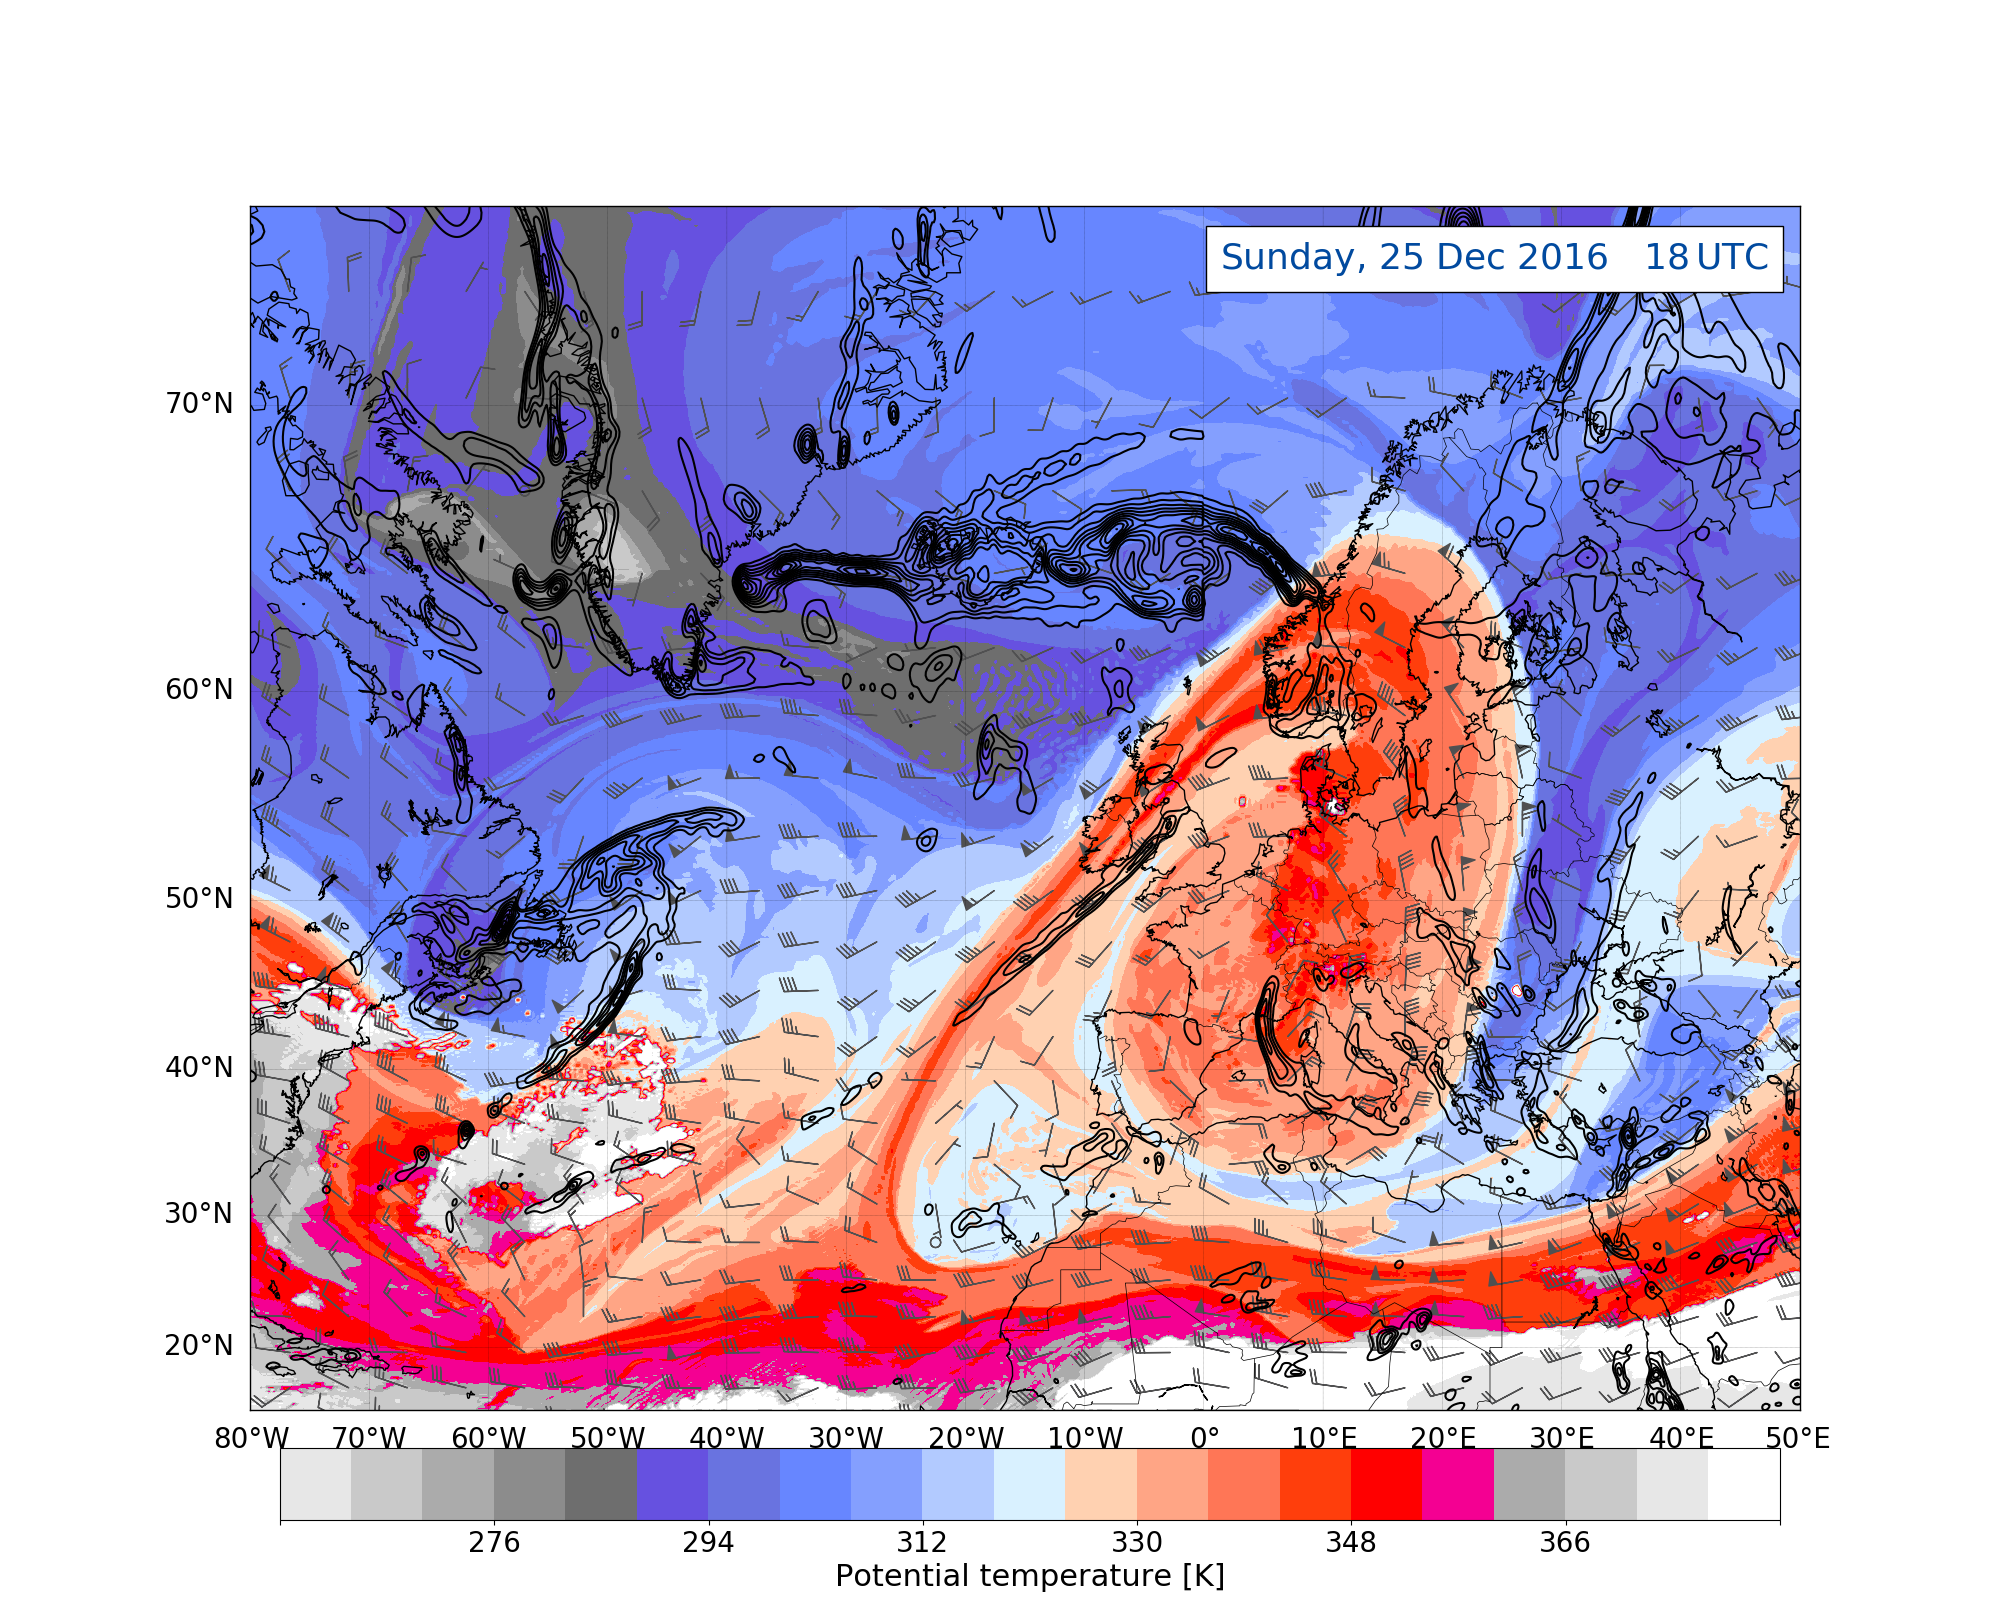
\includegraphics[trim={4.2cm 0cm 4.3cm 5.1cm},clip,
		width=\textwidth]{./fig_DynTropo/20161225_18}
		\caption{} \label{fig:DT25_18}
	\end{subfigure}
	%%% geopot %%%%
	\begin{subfigure}[b]{0.49\textwidth}
		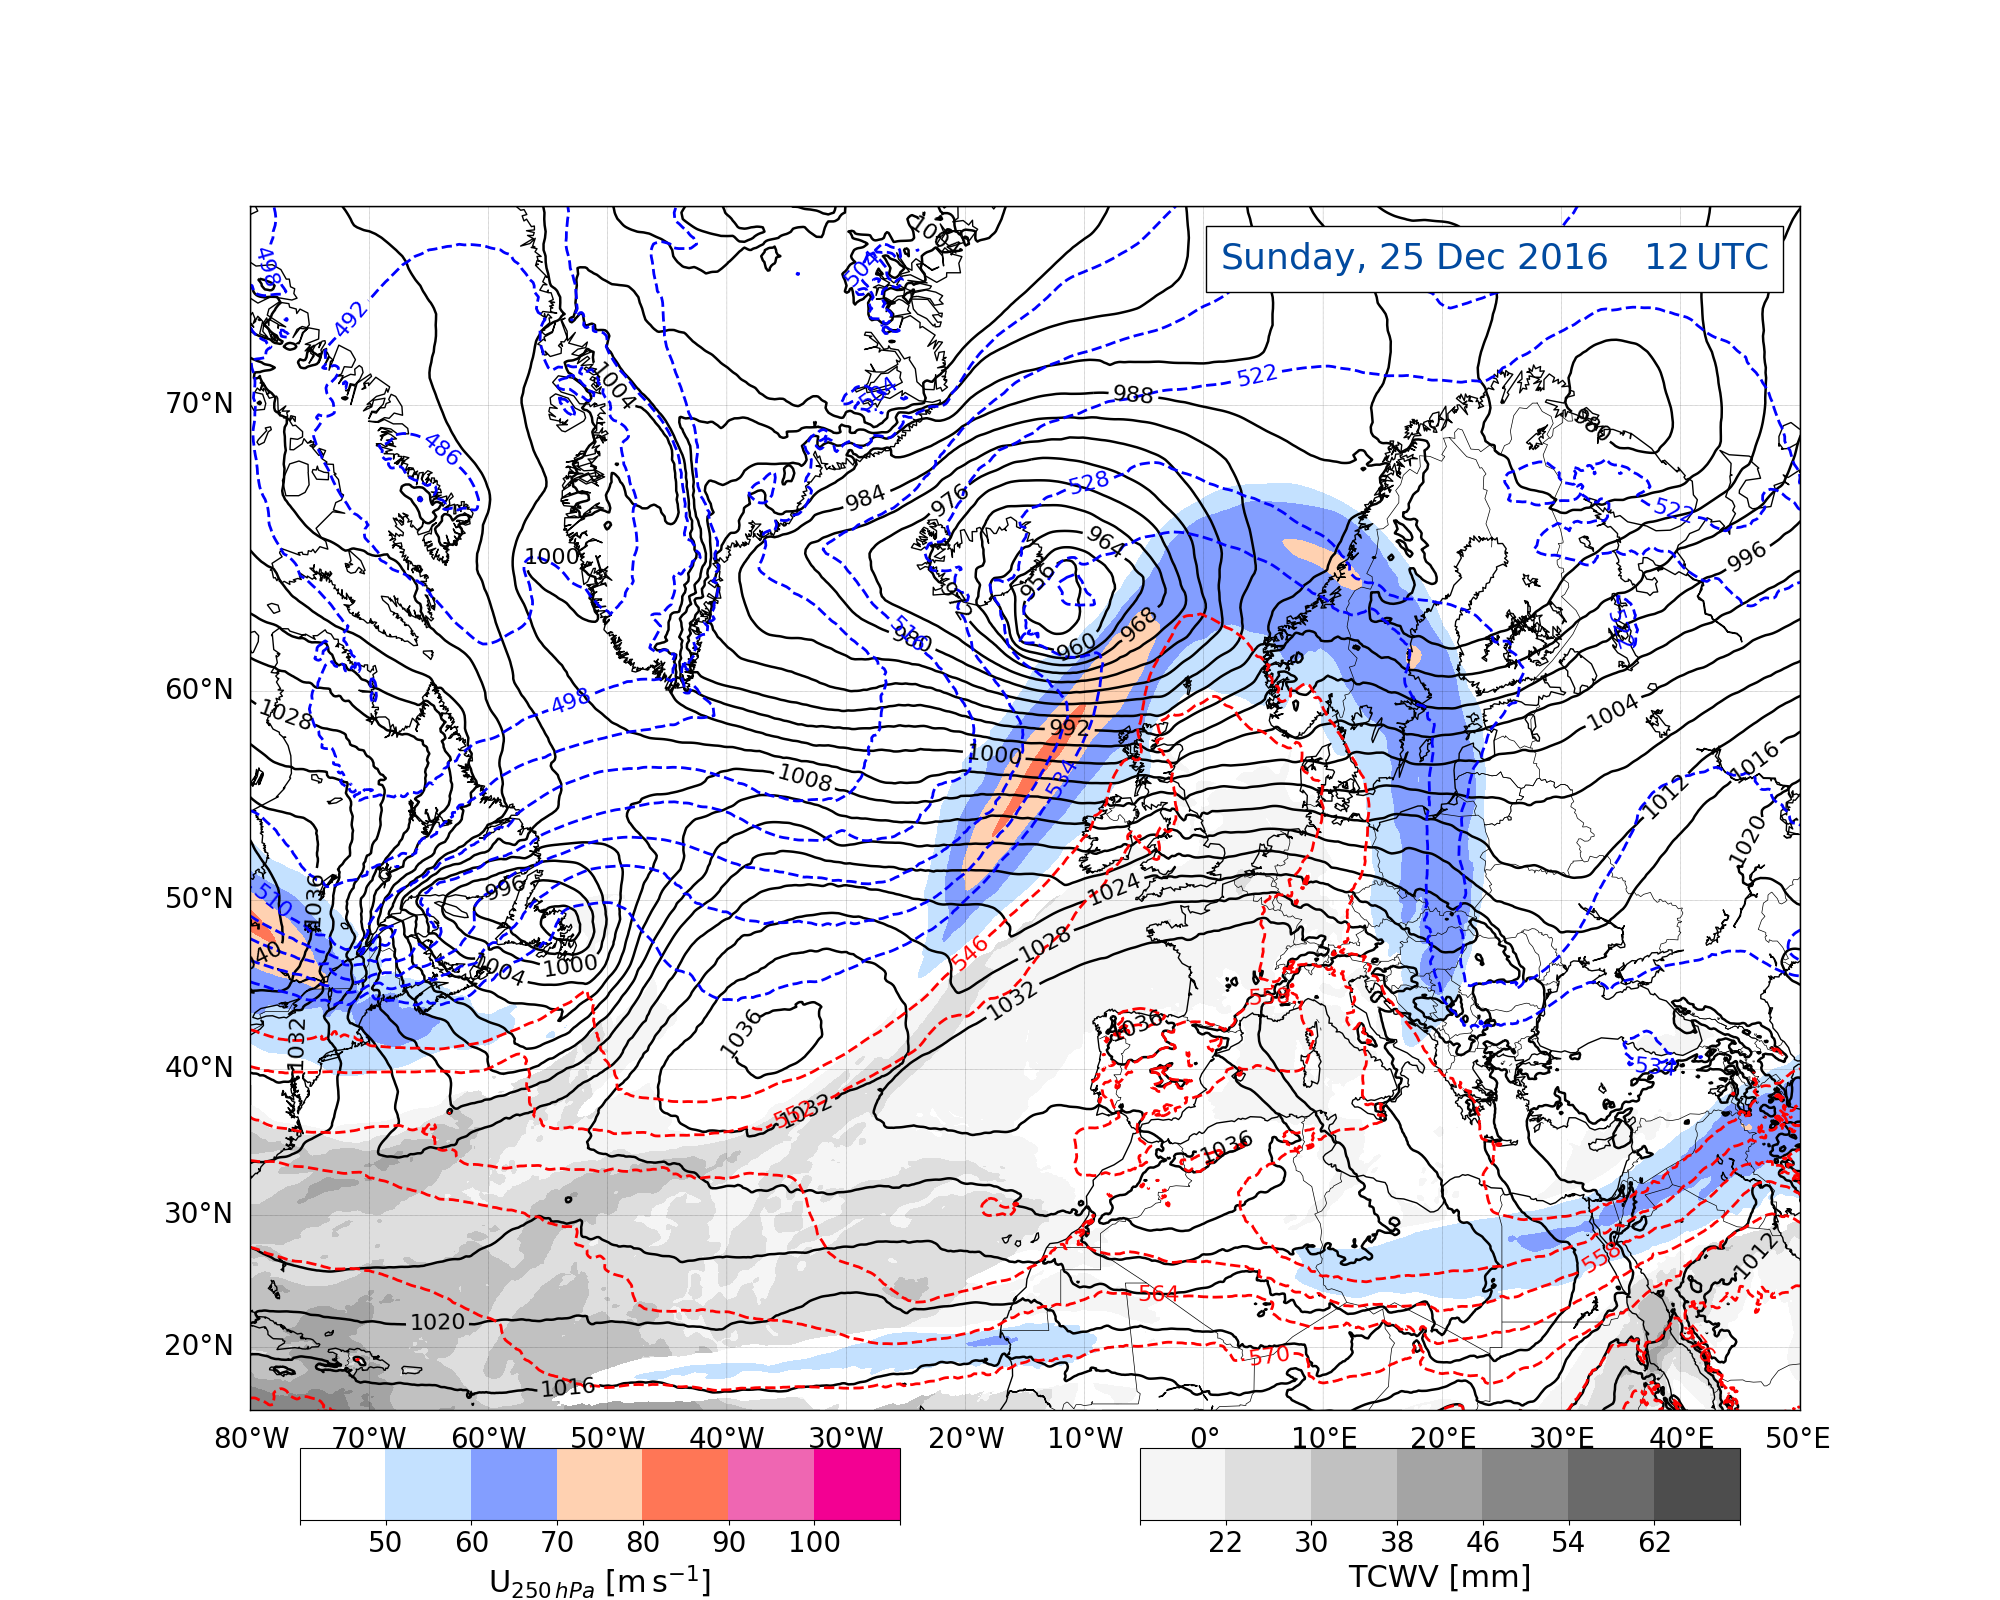
\includegraphics[trim={4.2cm 0cm 4.3cm 5.1cm},clip,
		width=\textwidth]{./fig_Geopot_Jet/20161225_12}
		\caption{} \label{fig:GP25}
	\end{subfigure}
	\begin{subfigure}[b]{0.49\textwidth}
		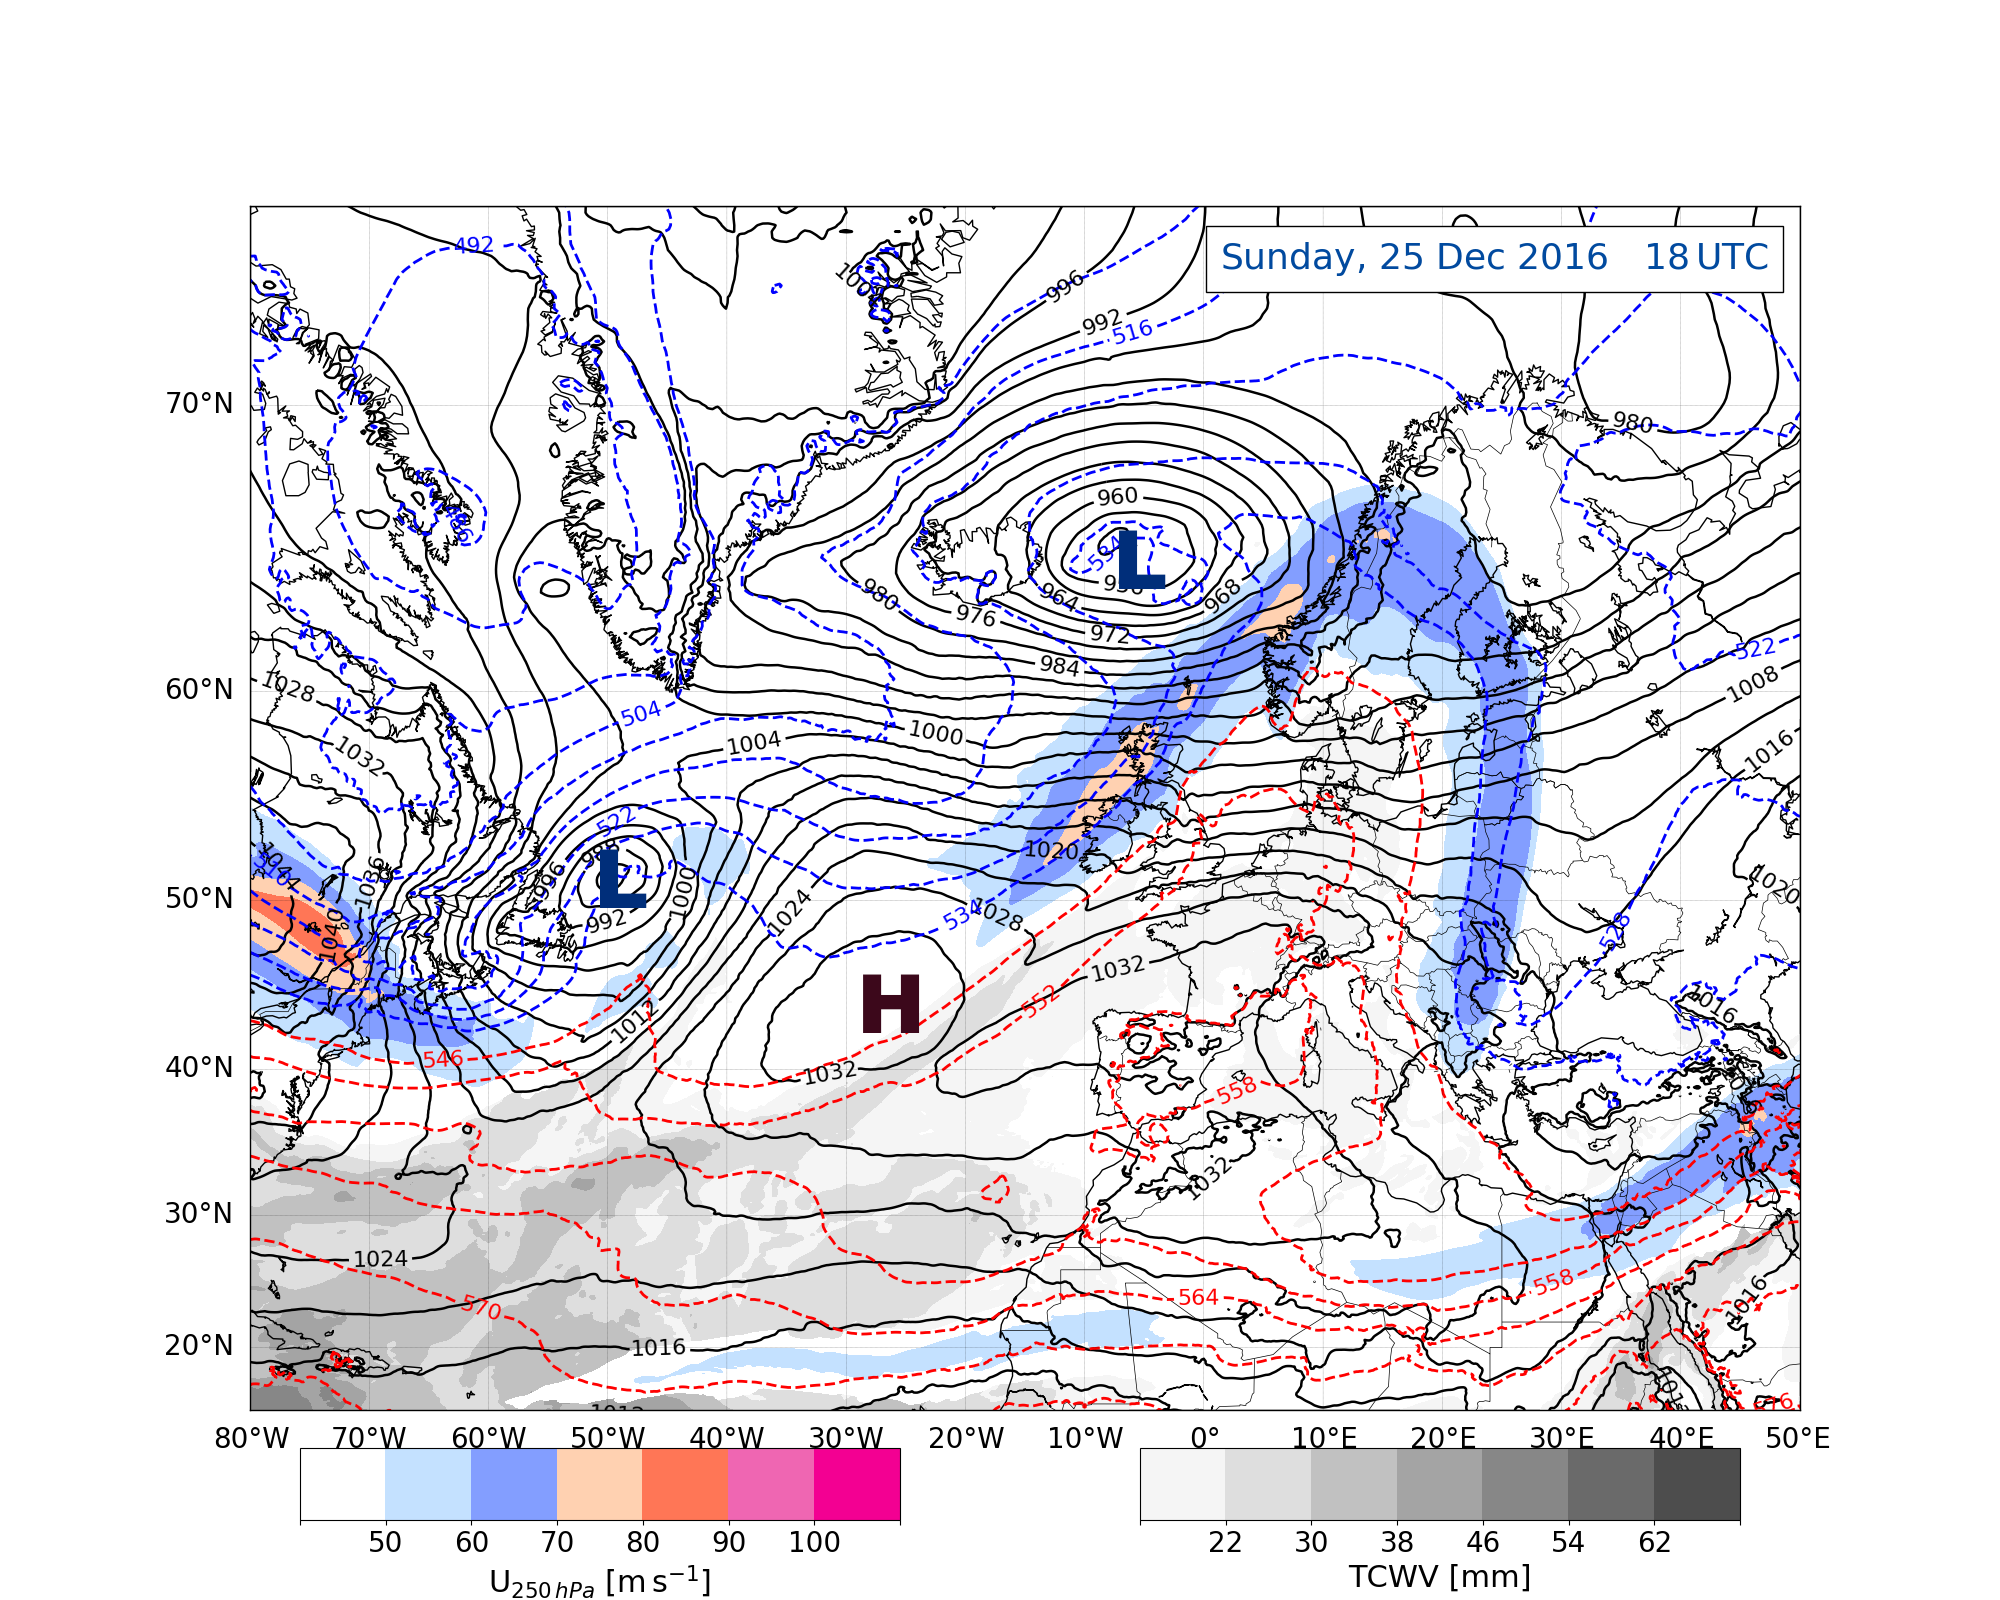
\includegraphics[trim={4.2cm 0cm 4.3cm 5.1cm},clip,
		width=\textwidth]{./fig_Geopot_Jet/20161225_18}
		\caption{} \label{fig:GP25_18}
	\end{subfigure}
	%%% local obs %%%%
	\begin{subfigure}[b]{0.49\textwidth}
		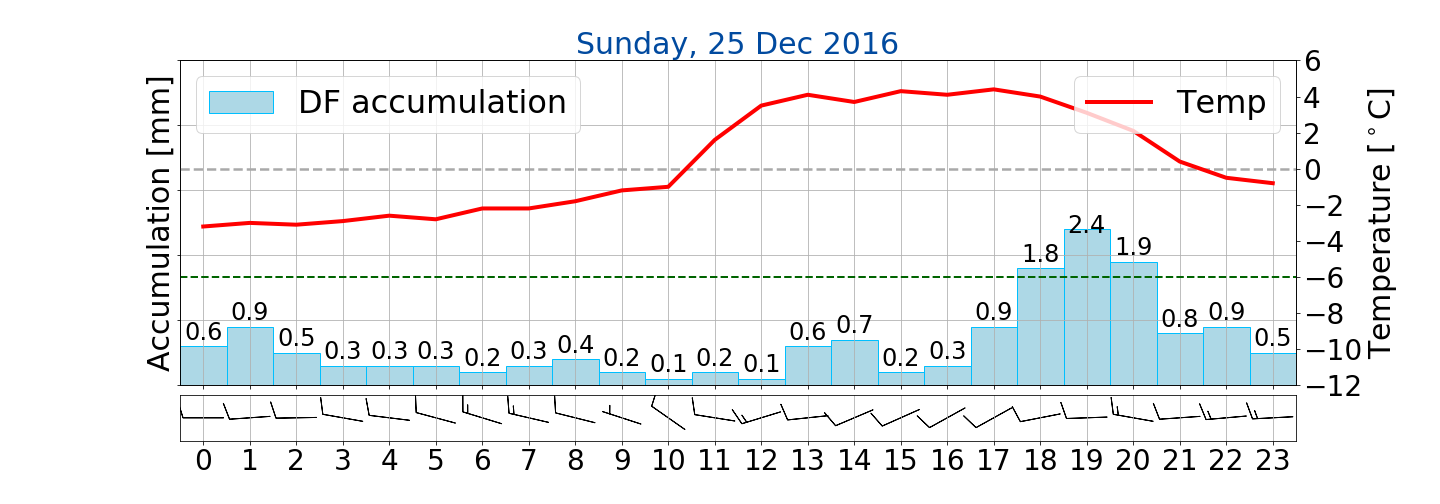
\includegraphics[trim={4.9cm 1.cm 1.5cm 1cm},clip,
		width=\textwidth]{./fig_weathermast/T_P_U_20161225}
		\caption{} \label{fig:TPU25}
	\end{subfigure}
\end{figure}
\subsection*{\SI{25}{\dec}}
%%% 25/12
% 25/00
% @ DT ridging coming in
% @ sfc, low with frontal boundaries
% Jet exit region is directly over Norway → Haukeliseter on right exit region? → sinking?
% Some orographic lifting
% 25/12
% Warm front comes through
% → low-level vorticity → orographic lifting
% 25/18
% Ridging bring more warm air to Norway (should be moist too → check total water vapor)
% Norway in warm sector
% Conducive westerly flow → orographic lifting
\textcolor{red}{Use the 00UTC and 12UTC analysis}
\noindent Twenty-four hours later the ridge is more pronounced and covers large parts of Norway. The surface low south-east of Iceland has built its frontal boundaries, which can be seen in the low-level vorticity of \Cref{fig:DT25}. The warm front lies west of Haukeliseter and starts to be observed at the measurement site (compare \Cref{fig:TPU25} for \SI{25}{\dec}). \Cref{fig:AR25} indicating the integrated vapour transport shows that a lot of moisture is transported from the Atlantic, towards Great Britain and south-western Norway. Together with the lifting at the surface boundary a sufficient amount of precipitation is observed. 
\\
Since the ridging brings moister (\Cref{fig:AR25}), warm air (\Cref{fig:DT25}) and Norway lies in a warm sector (\Cref{fig:GP25}) the assumption will be made, that the precipitation changed from solid to liquid. 

\begin{figure}
	\centering
	%%% dyntropo %%%%
	\begin{subfigure}[b]{0.49\textwidth}
		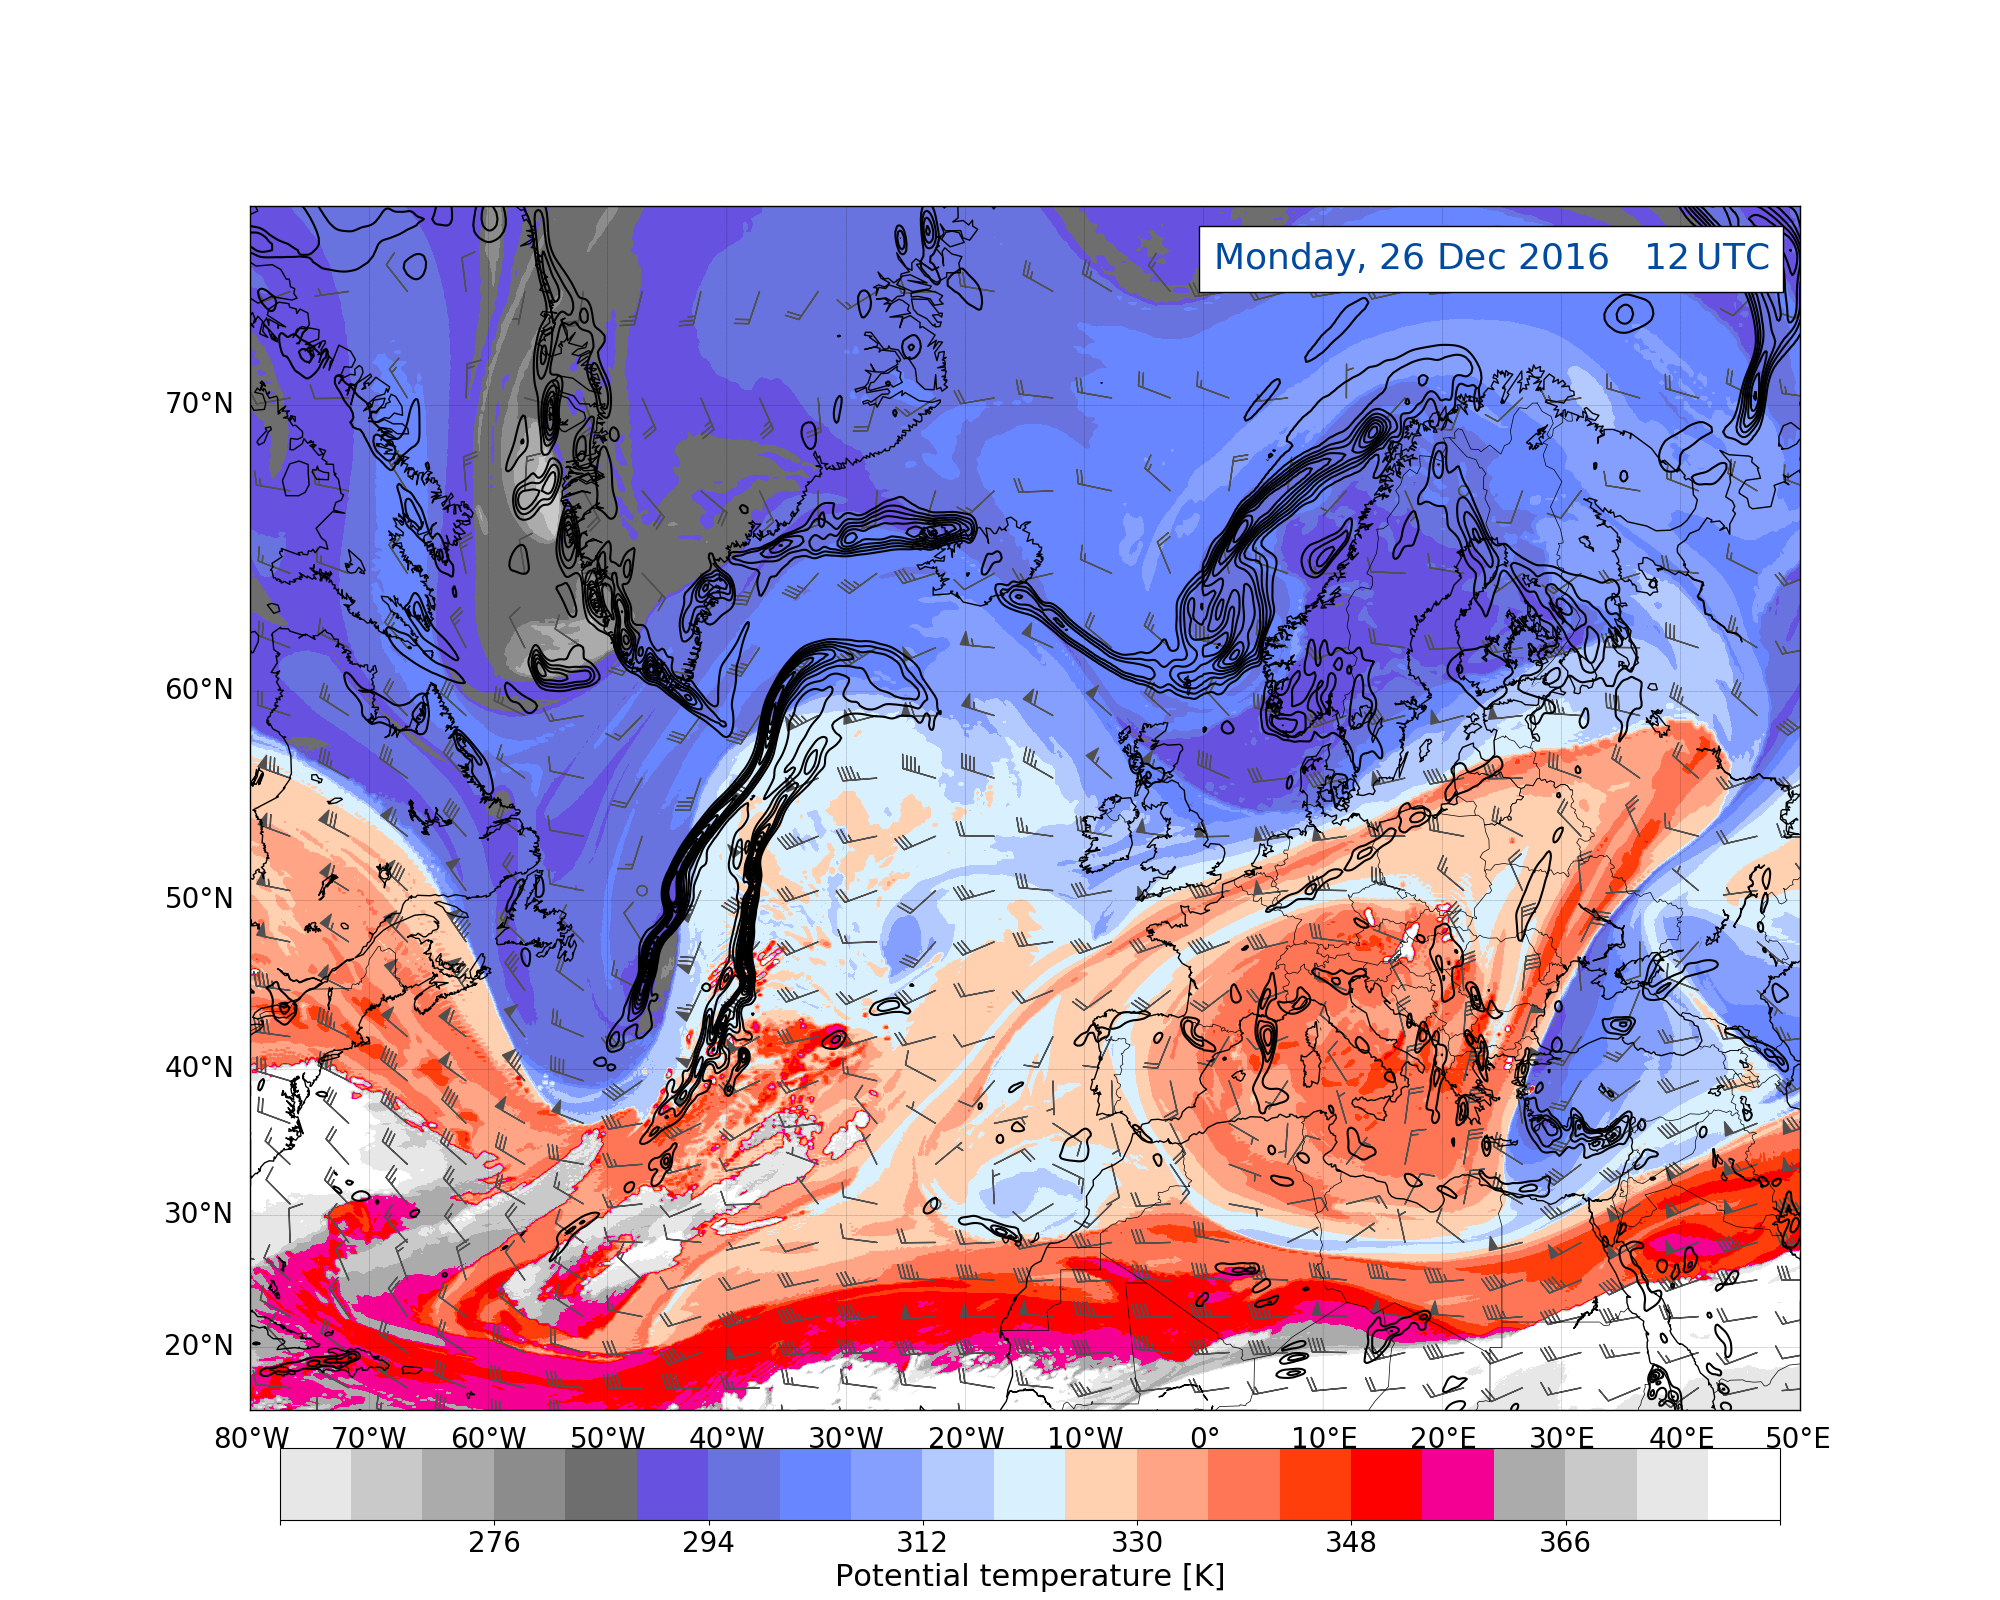
\includegraphics[trim={4.2cm 0cm 4.3cm 5.1cm},clip,
		width=\textwidth]{./fig_DynTropo/20161226_12}
		\caption{} \label{fig:DT26}
	\end{subfigure}
	\begin{subfigure}[b]{0.49\textwidth}
		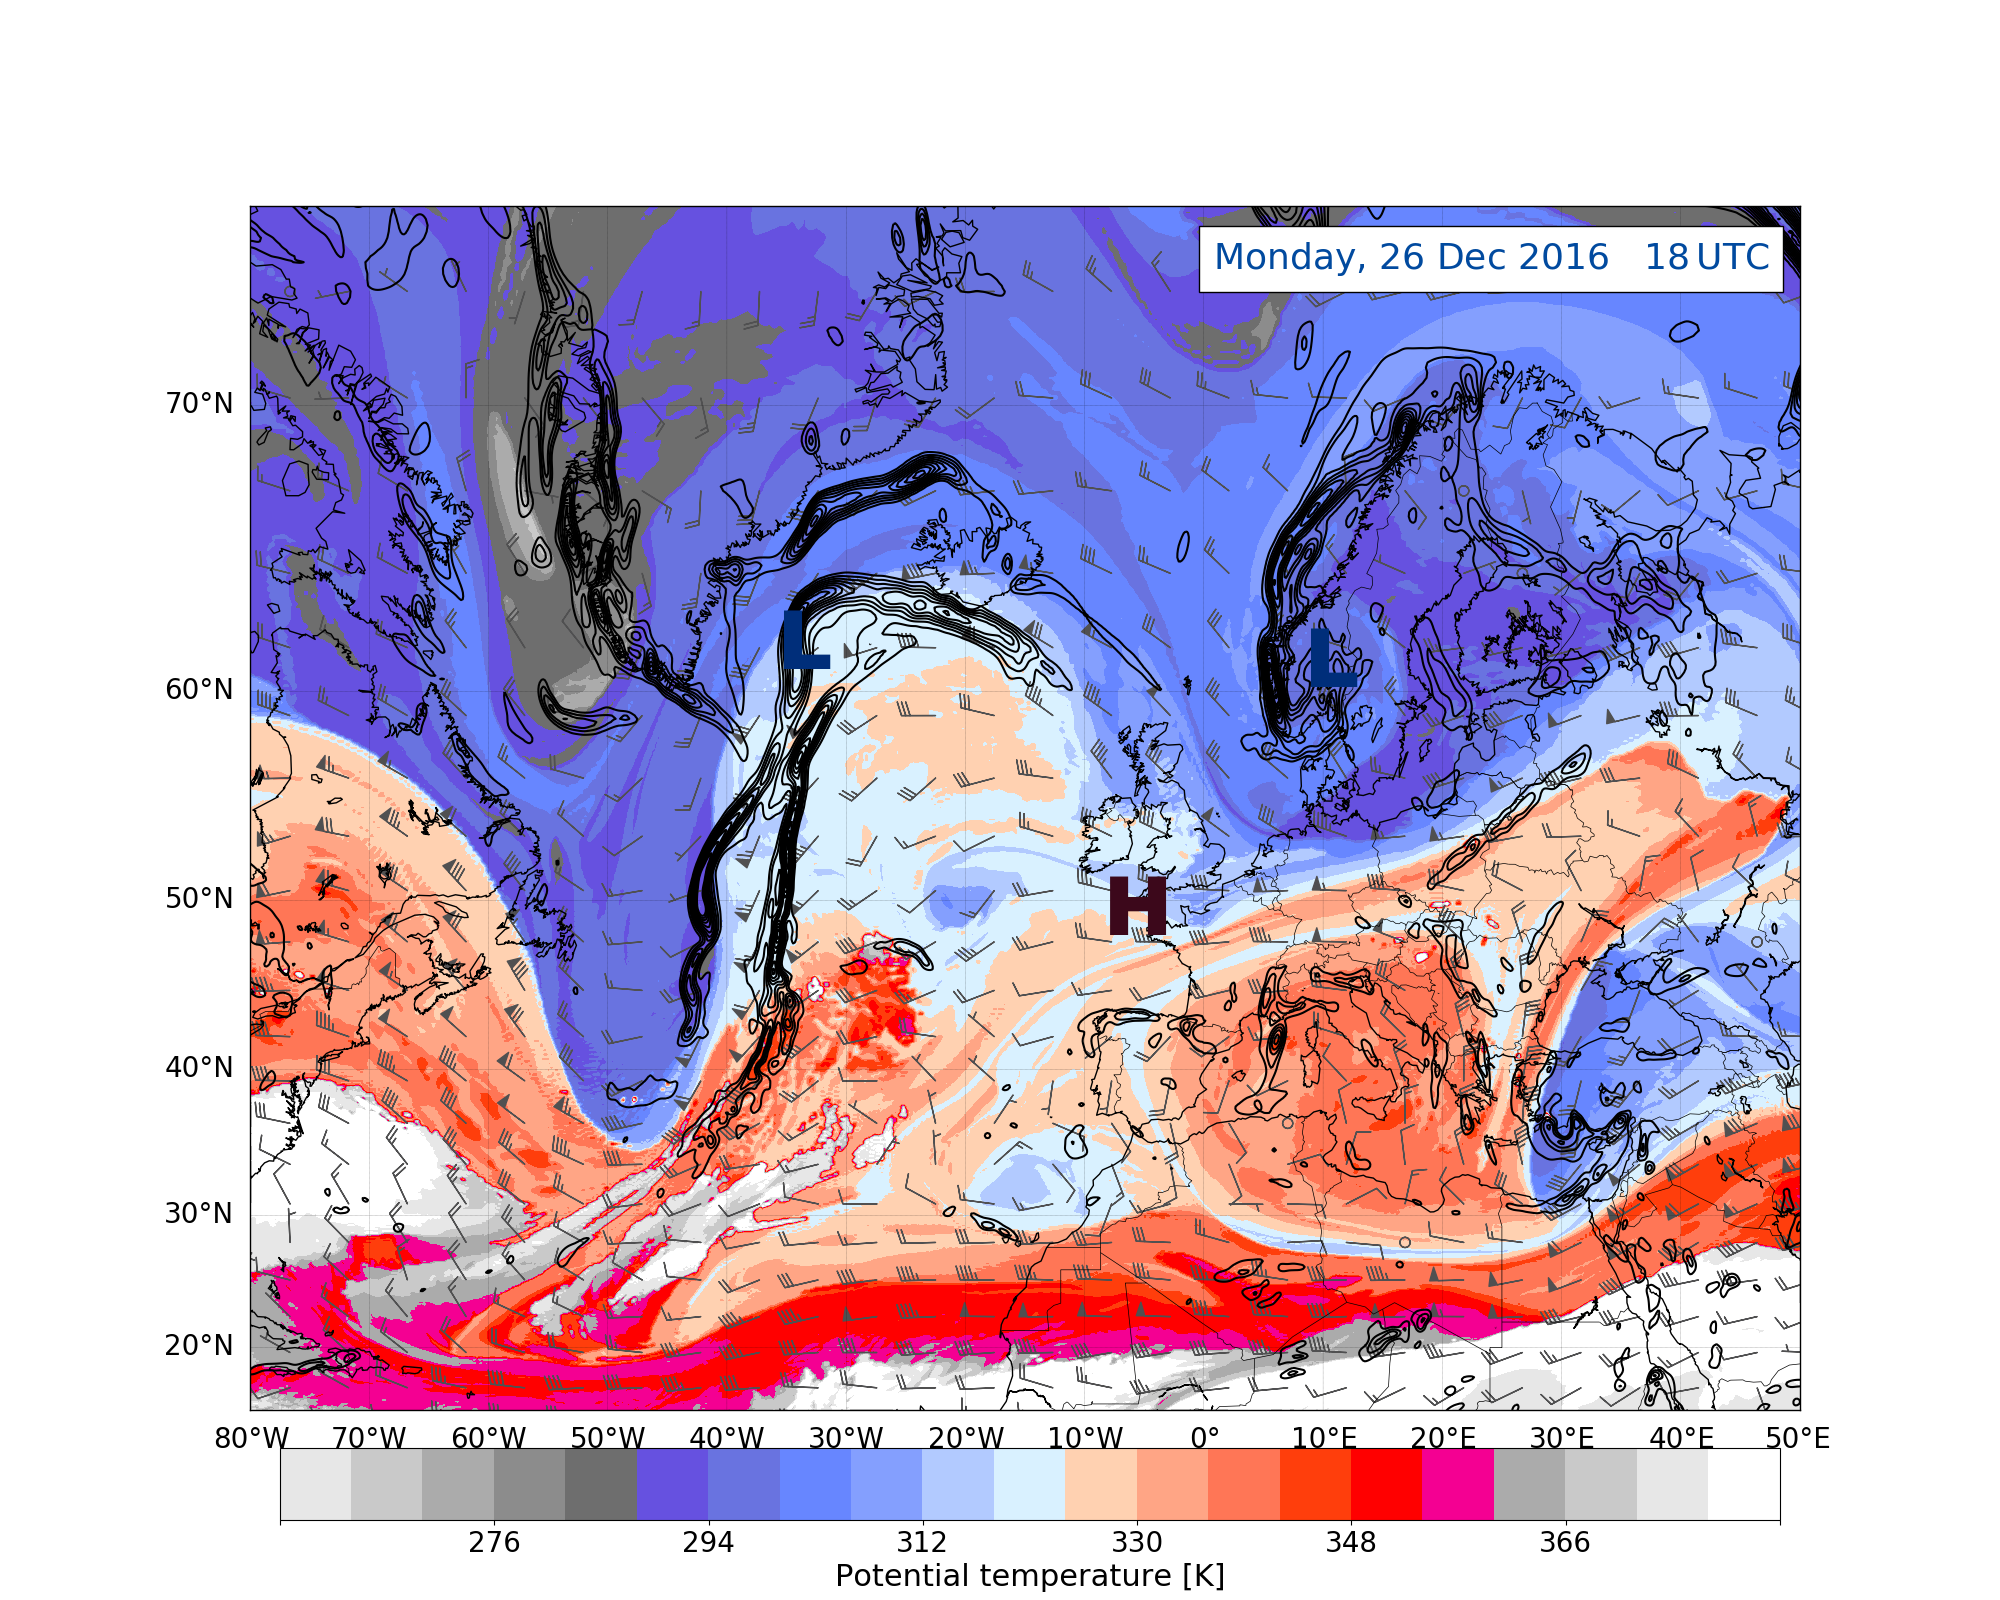
\includegraphics[trim={4.2cm 0cm 4.3cm 5.1cm},clip,
		width=\textwidth]{./fig_DynTropo/20161226_18}
		\caption{} \label{fig:DT26_18}
	\end{subfigure}
	%%% geopot %%%%
	\begin{subfigure}[b]{0.49\textwidth}
		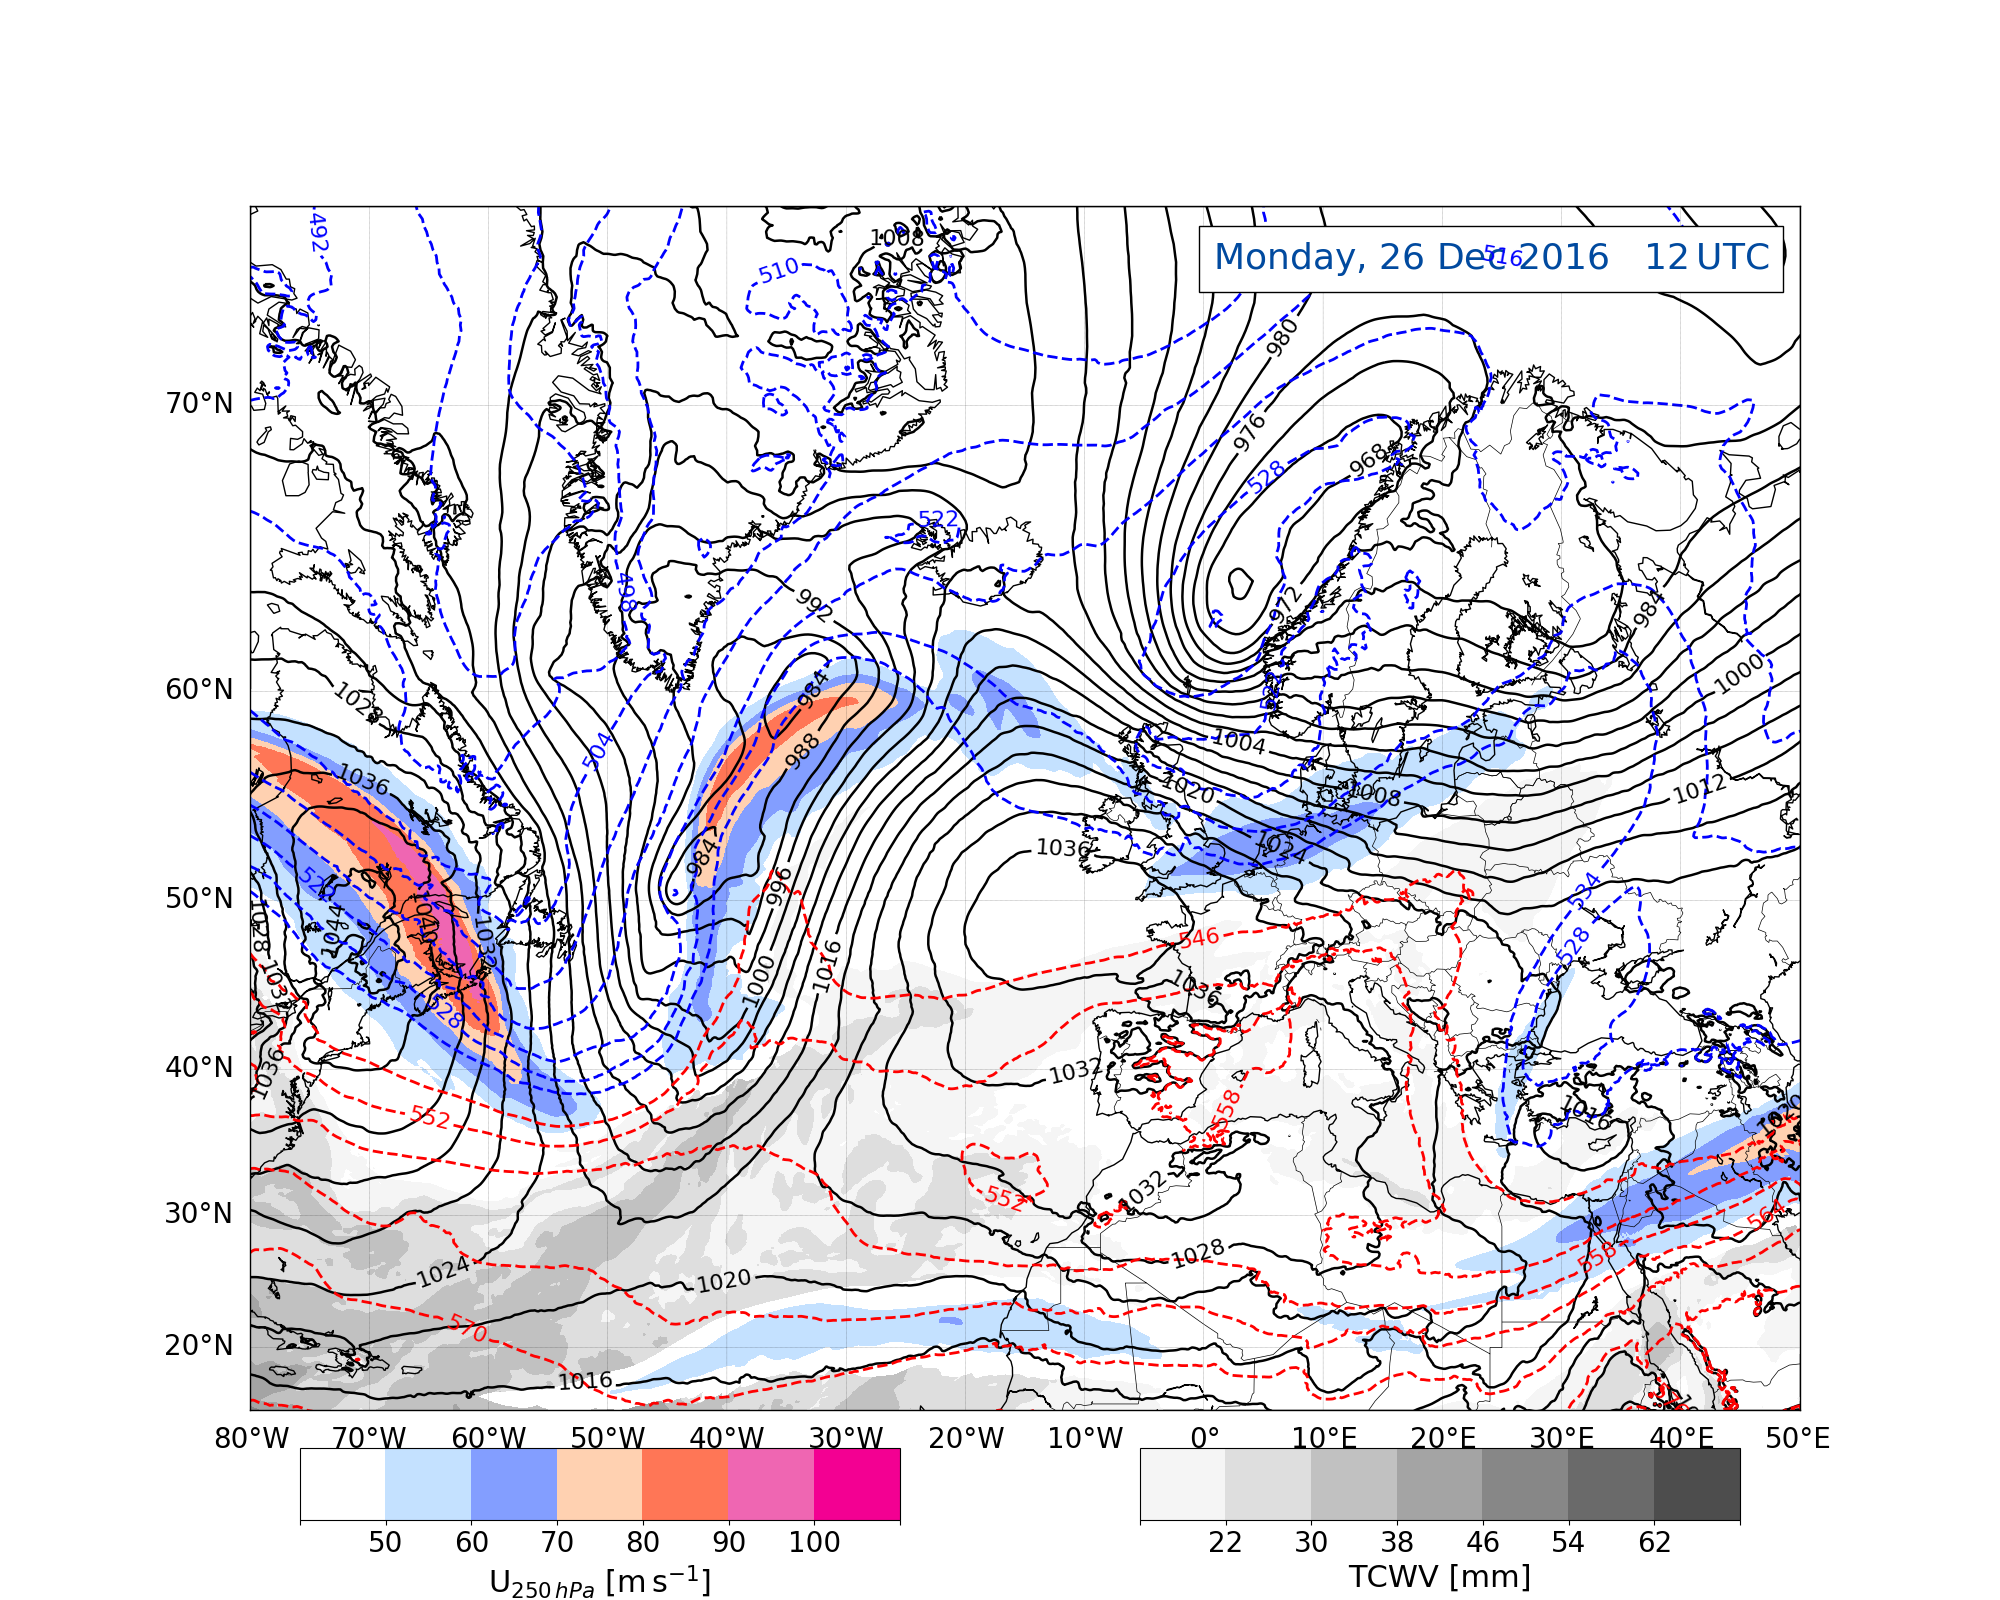
\includegraphics[trim={4.2cm 0cm 4.3cm 5.1cm},clip,
		width=\textwidth]{./fig_Geopot_Jet/20161226_12}
		\caption{} \label{fig:GP26}
	\end{subfigure}
	\begin{subfigure}[b]{0.49\textwidth}
		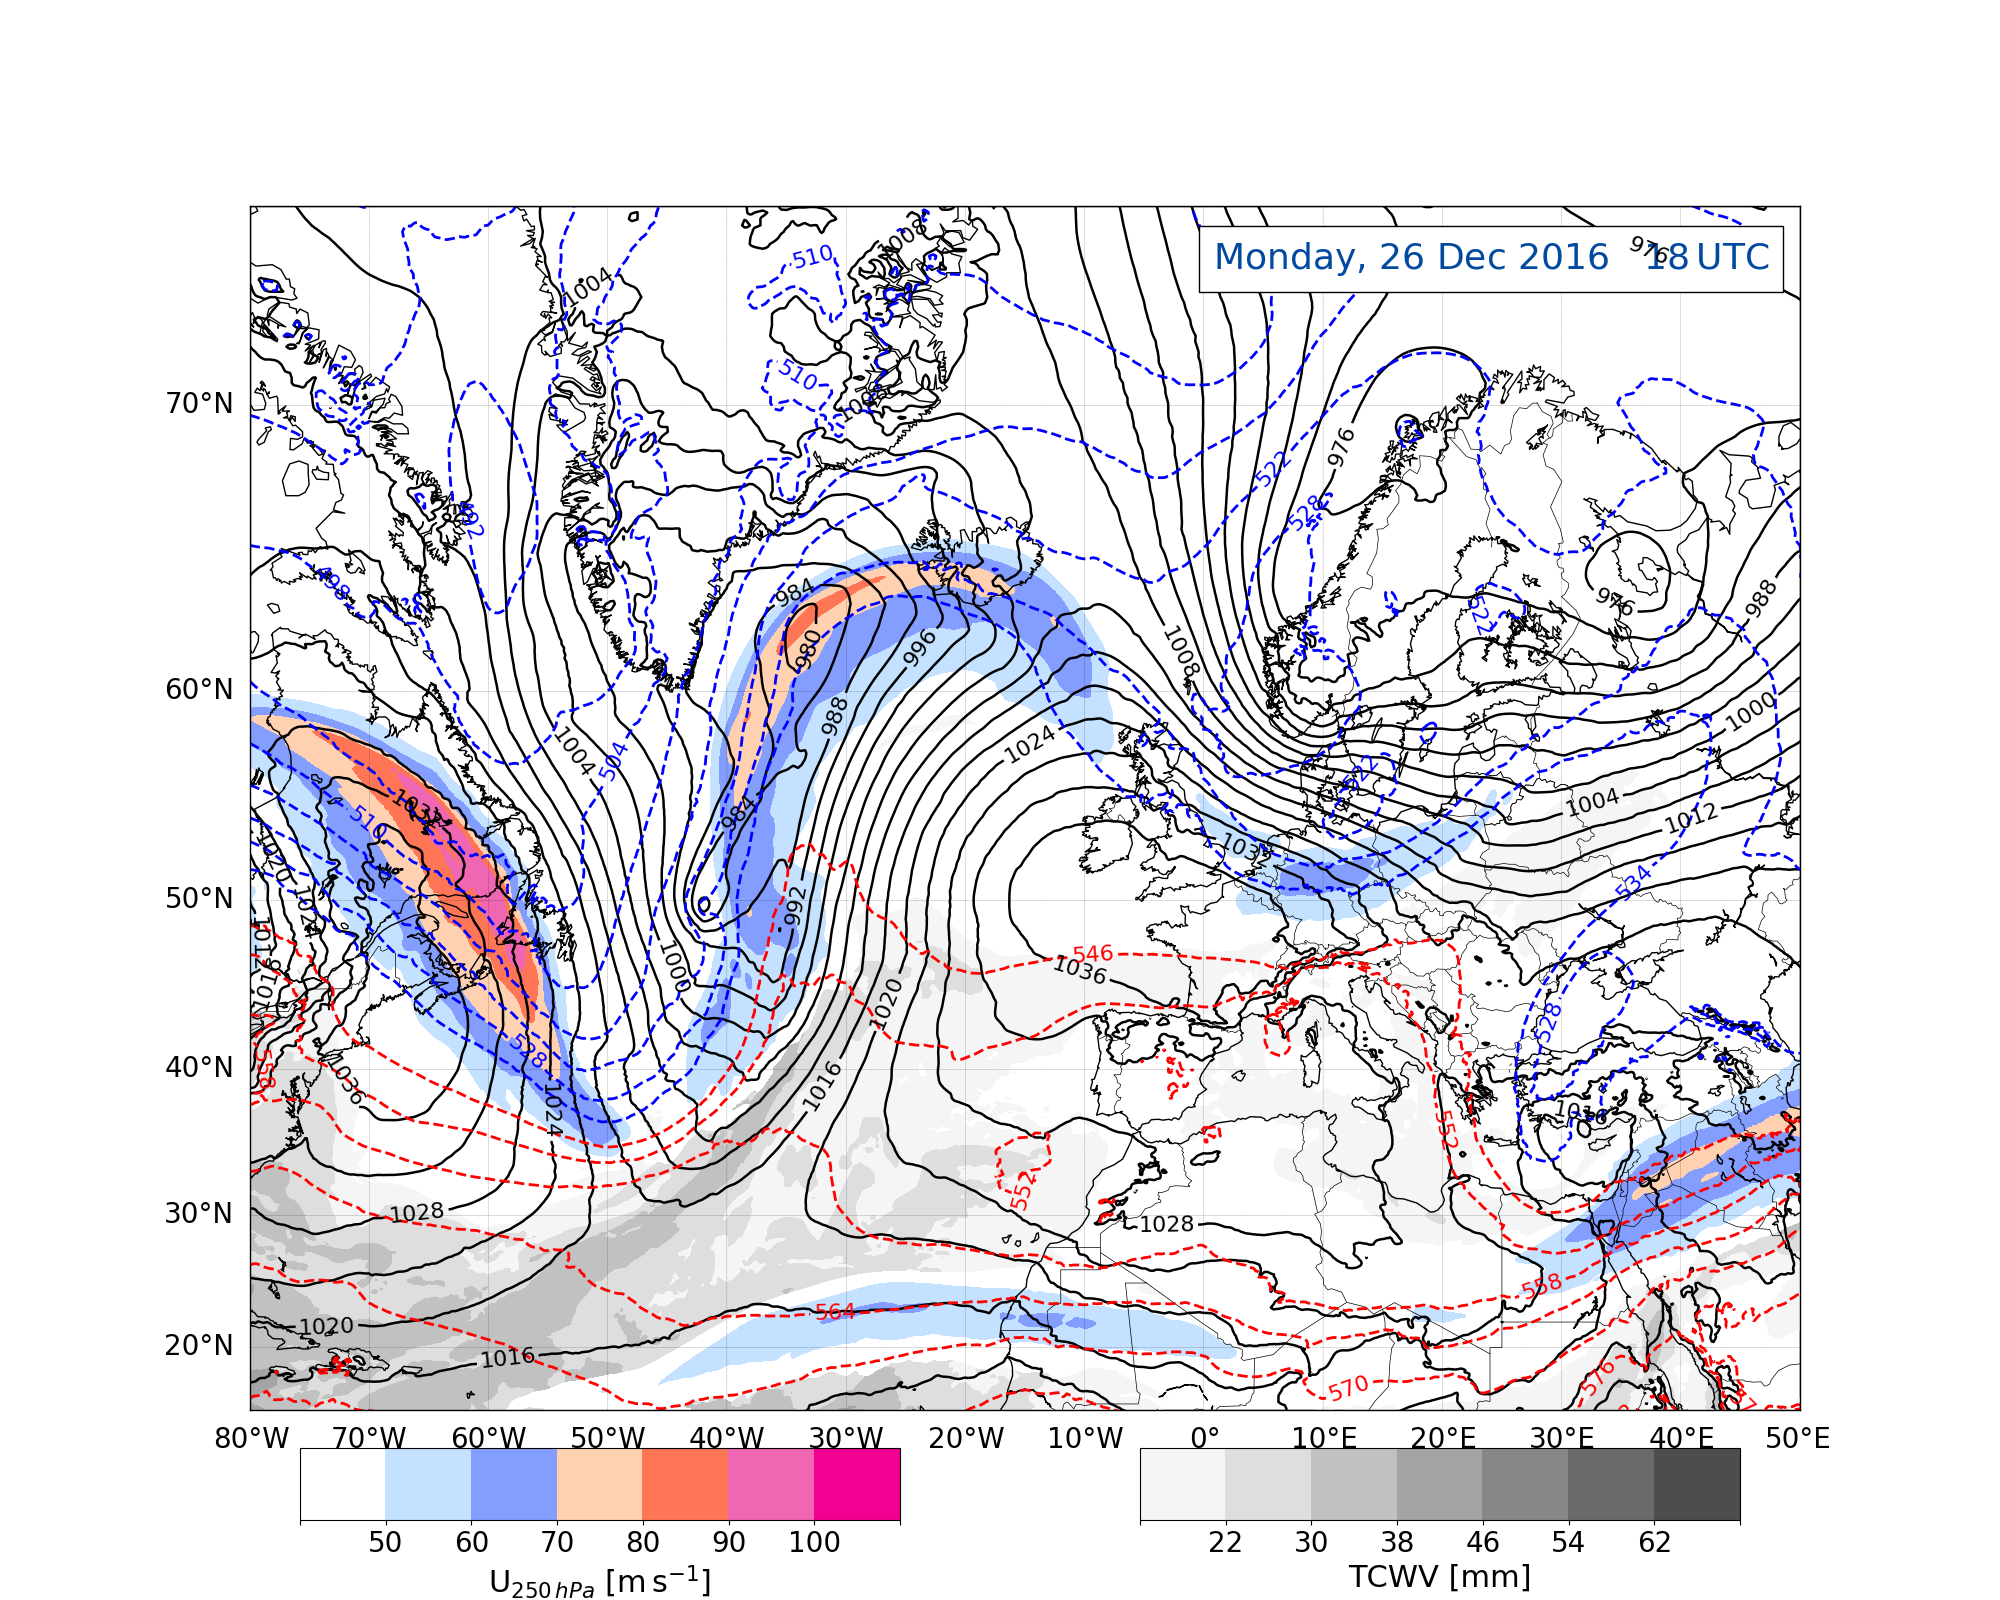
\includegraphics[trim={4.2cm 0cm 4.3cm 5.1cm},clip,
		width=\textwidth]{./fig_Geopot_Jet/20161226_18}
		\caption{} \label{fig:GP26_18}
	\end{subfigure}
	%%% local obs %%%%
	\begin{subfigure}[b]{0.49\textwidth}
		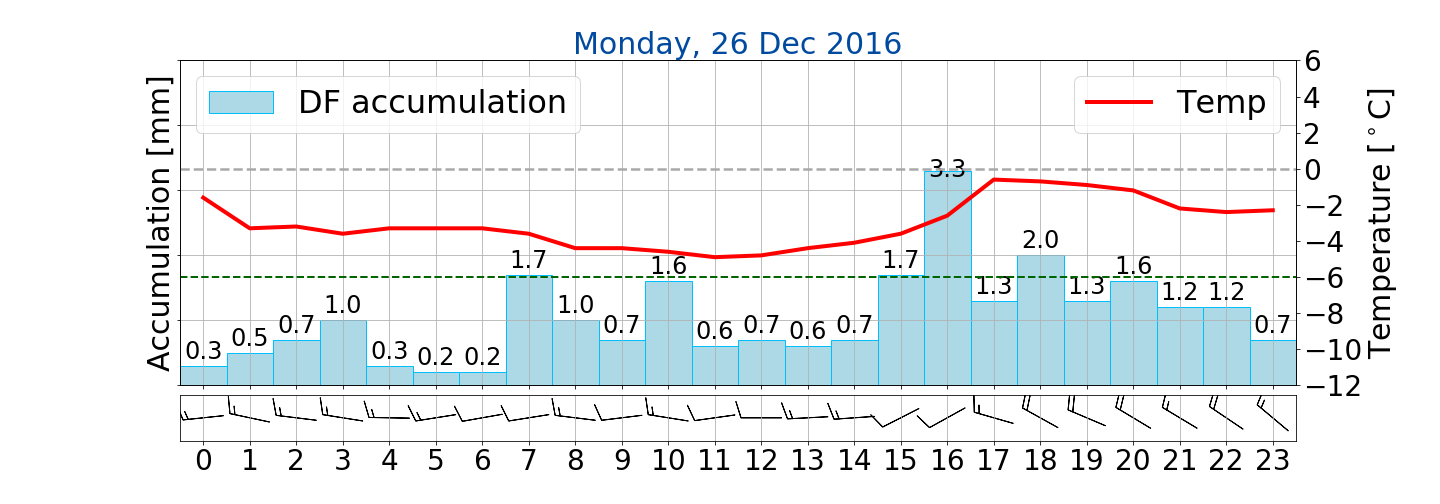
\includegraphics[trim={4.9cm 1.cm 1.5cm 1cm},clip,
		width=\textwidth]{./fig_weathermast/T_P_U_20161226}
		\caption{} \label{fig:TPU26}
	\end{subfigure}
\end{figure}
\subsection*{\SI{26}{\dec}}
%%% 26/12
% 26/06
% Cold front went through
% Norway lies in cold area (@ sfc: blue thickness lines, @ DT: cold anomaly)
% 26/18
% North westerly flow at west coast of Norway
% Conducive for orographic lifting, @ DT: strong low-level vorticity gradient
\textcolor{red}{Use the 12UTC and 18UTC analysis}
\noindent Within the next twenty-four hours the cold front passed through (temperature change in \Cref{fig:TPU26} for \SIrange{25}{26}{\dec}). Norway is covered in cold air (\Cref{fig:DT26}). The surface low-level indicates the occlusion of the cyclone and therefore a weakening. The wind is still from the west which is helpful for orographic lifting. The moisture content is still present but much weaker and smaller in extend. Since Norway is covered in cold air, the temperature is below zero and the precipitation had to be solid. 

\subsection*{\SI{27}{\dec}}
%%% 27/12
\noindent
The images of \SI{27}{\dec} show that the storm passed and disappeared. Southern Norway lies in cold air (\Cref{fig:DT27}), but on the right exit region of the jet ($\rightarrow$ sinking motion of cold air), compare \ref{fig:GP27}. A small amount of moisture is present (\Cref{fig:AR27}). Because of the wind change from west to north-west follows that orographic lifting is not present and the precipitation amount decreases at the end of the storm. 



